%%%%%%%%%%%%%%%%%%%%%%%%%%%%%%%%%%%%%%%%%
% Masters/Doctoral Thesis 
% LaTeX Template
% Version 1.43 (17/5/14)
%
% This template has been downloaded from:
% http://www.LaTeXTemplates.com
%
% Original authors:
% Steven Gunn 
% http://users.ecs.soton.ac.uk/srg/softwaretools/document/templates/
% and
% Sunil Patel
% http://www.sunilpatel.co.uk/thesis-template/
%
% License:
% CC BY-NC-SA 3.0 (http://creativecommons.org/licenses/by-nc-sa/3.0/)
%
% Note:
% Make sure to edit document variables in the Thesis.cls file
%
%
% Modified and Adapted by Michael Lees 2020
%%%%%%%%%%%%%%%%%%%%%%%%%%%%%%%%%%%%%%%%%

%----------------------------------------------------------------------------------------
%	PACKAGES AND OTHER DOCUMENT CONFIGURATIONS
%----------------------------------------------------------------------------------------

\documentclass[11pt, oneside]{Thesis} % The default font size and one-sided printing (no margin offsets)

\graphicspath{{Images/}} % Specifies the directory where pictures are stored

\usepackage[square, numbers, comma, sort&compress]{natbib} % Use the natbib reference package - read up on this to edit the reference style; if you want text (e.g. Smith et al., 2012) for the in-text references (instead of numbers), remove 'numbers' 
\usepackage[ruled,vlined]{algorithm2e}
\usepackage{amsmath}
\usepackage{booktabs}
\usepackage[nameinlink]{cleveref}
\PassOptionsToPackage{hyphens}{url}
\usepackage{hyperref}
\usepackage{array}
\usepackage{amsmath}
\usepackage[svgnames]{xcolor}
\usepackage{textcomp}
\usepackage[font=small,labelfont=bf]{caption}
\usepackage{float}
\usepackage{subcaption}

\usepackage{tabularx}
% \usepackage[margin=1in]{geometry} % Adjust margins if needed
\usepackage{booktabs}             % For better horizontal rules
\DeclareMathOperator*{\argmin}{arg\,min} 
\DeclareMathOperator*{\argmax}{arg\,max}
\hypersetup{urlcolor=black, colorlinks=true} % Colors hyperlinks in blue - change to black if annoying
\title{\ttitle} % Defines the thesis title - don't touch this
\begin{document}
\frontmatter % Use roman page numbering style (i, ii, iii, iv...) for the pre-content pages
\setstretch{1.3} % Line spacing of 1.3

% Define the page headers using the FancyHdr package and set up for one-sided printing
\fancyhead{} % Clears all page headers and footers
\rhead{\thepage} % Sets the right side header to show the page number
\lhead{} % Clears the left side page header

\pagestyle{fancy} % Finally, use the "fancy" page style to implement the FancyHdr headers

\newcommand{\HRule}{\rule{\linewidth}{0.5mm}} % New command to make the lines in the title page

% PDF meta-data
\hypersetup{pdftitle={\ttitle}}
\hypersetup{pdfsubject=\subjectname}
\hypersetup{pdfauthor=\authornames}
\hypersetup{pdfkeywords=\keywordnames}

%----------------------------------------------------------------------------------------
%	TITLE PAGE
%----------------------------------------------------------------------------------------

\begin{titlepage}
\begin{center}

\textsc{\LARGE \univname}\\[1.5cm] % University name
\textsc{\Large Masters Thesis}\\[0.5cm] % Thesis type

\HRule \\[0.4cm] % Horizontal line
{\huge \bfseries \ttitle}\\[0.4cm] % Thesis title
\HRule \\[1.5cm] % Horizontal line
 
\begin{minipage}{0.4\textwidth}
\begin{flushleft} \large
\emph{Author:}\\
\authornames % Author name - remove the \href bracket to remove the link
\end{flushleft}
\end{minipage}
\begin{minipage}{0.4\textwidth}
\begin{flushright} \large
\emph{Examiner:} \\
{\exname}\\
\emph{Supervisor:} \\
{\supname}\\
\emph{Assessor:} \\
{\assessorname}
\end{flushright}
\end{minipage}\\[1cm]
 
\large \textit{A thesis submitted in partial fulfillment of the requirements\\ for the degree of \degreename}\\[0.3cm] % University requirement text
\textit{in the}\\[0.4cm]
\groupname\\\deptname\\[1cm] % Research group name and department name
 
{\large \todayy}\\[2cm] % Date

\includegraphics[width=0.6\textwidth]{clslogo.png} % Include Computational Science Logo
 
\vfill
\end{center}

\end{titlepage}

%----------------------------------------------------------------------------------------
%	DECLARATION PAGE
%	Your institution may give you a different text to place here
%----------------------------------------------------------------------------------------

\Declaration{

\addtocontents{toc}{\vspace{1em}} % Add a gap in the Contents, for aesthetics

I, \authornames, declare that this thesis, entitled `\ttitle' and the work presented in it are my own. I confirm that:

\begin{itemize} 
\item[\tiny{$\blacksquare$}] This work was done wholly or mainly while in candidature for a research degree at the University of Amsterdam.
\item[\tiny{$\blacksquare$}] Where any part of this thesis has previously been submitted for a degree or any other qualification at this University or any other institution, this has been clearly stated.
\item[\tiny{$\blacksquare$}] Where I have consulted the published work of others, this is always clearly attributed.
\item[\tiny{$\blacksquare$}] Where I have quoted from the work of others, the source is always given. With the exception of such quotations, this thesis is entirely my own work.
\item[\tiny{$\blacksquare$}] I have acknowledged all main sources of help.
\item[\tiny{$\blacksquare$}] Where the thesis is based on work done by myself jointly with others, I have made clear exactly what was done by others and what I have contributed myself.\\
\end{itemize}


Signed: \\\\
\includegraphics[width=3cm]{Images/signature.pdf} \\
%\rule[1em]{25em}{0.5pt} % This prints a line for the signature
 
Date: \today\\
%\rule[1em]{25em}{0.5pt} % This prints a line to write the date
}

\clearpage % Start a new page

%----------------------------------------------------------------------------------------
%	QUOTATION PAGE
%----------------------------------------------------------------------------------------

\pagestyle{empty} % No headers or footers for the following pages

\null\vfill % Add some space to move the quote down the page a bit

% \textit{``What I cannot create, I do not understand.``}
\textit{``All models are wrong, but some are useful``}

% \begin{flushright}
%     Richard P. Feynman
% \end{flushright}
\begin{flushright}
    George E. P. Box
\end{flushright}

\vfill\vfill\vfill\vfill\vfill\vfill\null % Add some space at the bottom to position the quote just right

\clearpage % Start a new page

%----------------------------------------------------------------------------------------
%	ABSTRACT PAGE
%----------------------------------------------------------------------------------------

\addtotoc{Abstract} % Add the "Abstract" page entry to the Contents

\abstract{\addtocontents{toc}{\vspace{1em}} % Add a gap in the Contents, for aesthetics

Include your abstract here 
Abstracts must include sufficient information for reviewers to judge the nature and significance
of the topic, the adequacy of the investigative strategy, the nature of the results, and the
conclusions. The abstract should summarize the substantive results of the work and not merely
list topics to be discussed. 
Length 200-400 words.
}

\clearpage % Start a new page

%----------------------------------------------------------------------------------------
%	ACKNOWLEDGEMENTS
%----------------------------------------------------------------------------------------

\setstretch{1.3} % Reset the line-spacing to 1.3 for body text (if it has changed)

\acknowledgements{\addtocontents{toc}{\vspace{1em}} % Add a gap in the Contents, for aesthetics

% Thank the people that have helped, supervisors family etc.
I would like to thank my parents for eternally loving me and for financially supporting me through my Bachelor and Master studies, for without them, I wouldn't know where my life would be right now. 
Thank you to Dr. Matti Gralka for the weekly meetings and teaching me everything about phages and bacteria. 
Every meeting was always insightful, productive, and informative. 
I will forever be amazed at how he can remember which paper talks about which topic, and how he always had a paper for every topic. 
Thank you to Sofia Blaszczyk for finding this opening and suggesting that I email Dr. Gralka for an introductory meeting, and for acting as my \href{https://www.wikiwand.com/en/articles/Rubber_duck_debugging}{rubber duck programming buddy}, and watching my cringe screen recordings that I sent her at 2am showcasing various demos of my code. 
If I hadn't followed Dr. Rik Kaasschieter's and Dr. Martijn Anthonissen's courses “Introduction Computational Sciences“ and “Numerical Linear Algebra“ in my Bachelors, I would not have been interested in Computational Sciences and would not have found the MSc Computational Sciences program, as Computational Sciences fits my interests and skill sets better than any other program I could have taken. 
For they have forever altered my career trajectory. 
Thank you to Sarah Flickinger for showing me the research that she has been doing in the lab. 
She allowed me to really connect my research and models to real life, reminding me that what I am doing has real life use cases than just a purely theoretical or programming challenge. 
And finally, thank you to all of my friends for keeping me sane and helping me through both of my programs. 
}
\clearpage % Start a new page

%----------------------------------------------------------------------------------------
%	LIST OF CONTENTS/FIGURES/TABLES PAGES
%----------------------------------------------------------------------------------------

\pagestyle{fancy} % The page style headers have been "empty" all this time, now use the "fancy" headers as defined before to bring them back

\lhead{\emph{Contents}} % Set the left side page header to "Contents"
\tableofcontents % Write out the Table of Contents

\lhead{\emph{List of Figures}} % Set the left side page header to "List of Figures"
\listoffigures % Write out the List of Figures

\lhead{\emph{List of Tables}} % Set the left side page header to "List of Tables"
\listoftables % Write out the List of Tables

\lhead{\emph{List of Algorithms}} % Set the left side page header to "List of Algorithms"
\addtotoc{List of Algorithms}
\listofalgorithms % Write out the List of Tables

%----------------------------------------------------------------------------------------
%	ABBREVIATIONS
%----------------------------------------------------------------------------------------

\clearpage % Start a new page

\setstretch{1.5} % Set the line spacing to 1.5, this makes the following tables easier to read

\lhead{\emph{Abbreviations}} % Set the left side page header to "Abbreviations"
\listofsymbols{ll} % Include a list of Abbreviations (a table of two columns)
{
    \textbf{ABM} & \textbf{A}gent \textbf{B}ased \textbf{M}odelling \\ 
    \textbf{ARD} & \textbf{A}rms \textbf{R}ace \textbf{D}ynamic \\ 
    \textbf{BVP} & \textbf{B}oundary \textbf{V}alue \textbf{P}roblem \\ 
    \textbf{CBASS} & \textbf{C}yclic oligonucleotide-\textbf{B}ased \textbf{A}ntiphage \textbf{S}ignalling \textbf{S}ystems\\
    \textbf{CRISPR} & \textbf{C}lustered \textbf{R}egularly \textbf{I}nterspaced \textbf{S}hort \textbf{P}alindromic \textbf{R}epeats \\
    \textbf{DDE} & \textbf{D}elay \textbf{D}ifferential \textbf{E}quation \\ 
    \textbf{DNA} & \textbf{D}eoxyribo\textbf{N}ucleic \textbf{A}cid \\
    \textbf{FSD} & \textbf{F}luctuating \textbf{S}election \textbf{D}ynamics \\ 
    \textbf{GUI} & \textbf{G}raphical \textbf{U}ser \textbf{I}nterface \\ 
    \textbf{OD} & \textbf{O}ptical \textbf{D}ensity \\ 
    \textbf{ODE} & \textbf{O}rdinary \textbf{D}ifferential \textbf{E}quation \\
    \textbf{PDE} & \textbf{P}artial \textbf{D}ifferential \textbf{E}quation \\ 
    \textbf{RNA} & \textbf{R}ibo\textbf{N}ucleic \textbf{A}cid\\
    \textbf{SIE} & \textbf{S}uper\textbf{I}nfection \textbf{E}xclusion \\
    \textbf{SNP} & \textbf{S}ingle \textbf{N}ucleotide \textbf{P}olymorphism \\
    \textbf{TAB} & \textbf{T}ail \textbf{A}ssembly \textbf{B}locker \\
    \textbf{UvA} & \textbf{U}niversitiet \textbf{v}an \textbf{A}msterdam\\
    }

%----------------------------------------------------------------------------------------
%	PHYSICAL CONSTANTS/OTHER DEFINITIONS
%----------------------------------------------------------------------------------------

\clearpage % Start a new page

%\lhead{\emph{Physical Constants}} % Set the left side page header to "Physical Constants"

%\listofconstants{lrcl} % Include a list of Physical Constants (a four column table)
%{
%Speed of Light & $c$ & $=$ & $2.997\ 924\ 58\times10^{8}\ \mbox{ms}^{-\mbox{s}}$ (exact)\\
%% Constant Name & Symbol & = & Constant Value (with units) \\
%}

%----------------------------------------------------------------------------------------
%	SYMBOLS
%----------------------------------------------------------------------------------------

%\clearpage % Start a new page

%\lhead{\emph{Symbols}} % Set the left side page header to "Symbols"

%\listofnomenclature{lll} % Include a list of Symbols (a three column table)
%{
%$a$ & distance & m \\
%$P$ & power & W (Js$^{-1}$) \\
%% Symbol & Name & Unit \\

%& & \\ % Gap to separate the Roman symbols from the Greek
%
%$\omega$ & angular frequency & rads$^{-1}$ \\
%% Symbol & Name & Unit \\
%}

%----------------------------------------------------------------------------------------
%	DEDICATION
%----------------------------------------------------------------------------------------

\setstretch{1.3} % Return the line spacing back to 1.3

\pagestyle{empty} % Page style needs to be empty for this page

\addtocontents{toc}{\vspace{2em}} % Add a gap in the Contents, for aesthetics

%----------------------------------------------------------------------------------------
%	THESIS CONTENT - CHAPTERS
%----------------------------------------------------------------------------------------

\mainmatter % Begin numeric (1,2,3...) page numbering

\pagestyle{fancy} % Return the page headers back to the "fancy" style

% Include the chapters of the thesis as separate tex files from the Chapters folder
% Change the file names if you prefer

%This structure provides a bare bones essentials of the thesis and some indicative length
%This structure may not fit your thesis perfectly, but be sure to include these components somehow.
%It is possible to split the chapters up (E.g., 2 methods chapter, Experiment and Results as two, etc.)

% The typical length may be between 43 - 64 pages. Do not worry if you go slightly larger or smaller than this. 
% But a thesis of 20 pages, or 100 pages may suggest you've been to brief or too verbose.
%NOTE - there is not strict limit/minimum.

\lhead{\emph{Introduction}}
\chapter{Introduction}
\label{Introduction}

Phages are small viruses on the order of 27-190nm that infect and lyse (kill) specific bacteria, acting as nature's natural anti-microbial defense. 
Researchers are attempting to determine how phages can be used in various medical and industrial applications to control bacterial growth. 
However, researchers need to know how the interactions between phages and bacteria work in order to implement a robust method to control bacterial growth. 

\section{Thesis Overview}
This thesis covers multiple topics to ultimately answer how phages and bacteria interactions can be mathematically modelled. 
First, there is a (biological) introduction to phages and bacteria. 
This introduction covers how phages work and infect bacteria, how bacteria defend against phages, how phages defeat bacterial defenses, and how phages defend against other phages. 
There is also an introduction to different modelling techniques such as spatial vs non-spatial models and ODEs vs DDEs. 
This thesis briefly covers software that models phages, resources, bacteria, and their limitations. 

This thesis presents software I developed to support the research, demonstrating its capabilities using a representative model of phage-bacteria-resource interactions. 
The section also provides an overview of its usage, including example outputs from demonstration runs.
Finally, the results generated by the software will be thoroughly analyzed and discussed.

\section{Biological Background}
Phages are small viruses on the order of 27-190nm (the average size of marine phages are 54nm) that infect and lyse (kill) specific bacteria.
Phages are so small, that it takes 55 million phages to cover the period at the end of this sentence \cite{breitbartPhagePuppetMasters2018}. 
The phage cycle process starts with a phage coming into contact with a bacterium.
Once it has identified an injection site, the phage can inject a strain of DNA into the bacteria.
The DNA strand has two options: it can either merge into the bacterial DNA, allowing the phage's DNA strand to replicate alongside the bacteria as they reproduce.
This process defines the Lysogenic cycle.
After a set amount of time, the DNA of the phage can unmerge and hijack the DNA replicating mechanism, creating multiple copies of itself, using the transcription, translation, and replication process to create multiple copies of itself.
The phages begin to self-assemble inside the bacteria until the bacteria is full of phages and explodes, the lysis stage, releasing the phages into the environment, ready to repeat the process again. 

This process can be visualized in \Cref{fig:phage_life_cycle}.
\begin{figure}
    \centering
    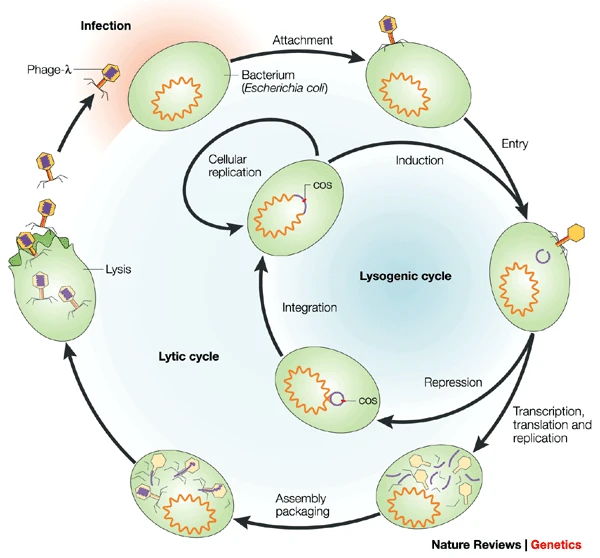
\includegraphics[width=0.5\linewidth]{Figures/phage_life_cycle.png}
    \caption{Life cycle of a phage, inside and outside a bacteria cell. Significant steps in the life cycle of a phage include the infection stage, integration, replication, and lysing process. Figure sourced from \citet{campbellFutureBacteriophageBiology2003}. }
    \label{fig:phage_life_cycle}
\end{figure}

\section{The Environment}
In an ecosystem like the ocean, the gut, or in soil, there are thousands of different microbes all interacting with one another or the surrounding environment.
The interactions are complex, with many factors affecting the growth of bacteria, phages, plants, animals, and more. 

The interactions between entities in the environment are often synergistic. 
When an animal dies, bacteria start to digest and decompose the animal into simpler chemicals like carbon and nitrogen that plants can use to grow, which is then eaten by other animals. 
External factors, such as flooding, droughts, chemical spills, or introduction of new entities have a massive impact on the ecosystem. 
These events can add or remove resources from the system, change environmental parameters such as the surrounding temperature, introduce competition, or create an imbalance in the population by killing entities. 
These effects have a larger effect on the ecosystem and food chain as a whole as bacteria are one of the fundamental foundations for resource recycling. 

\subsection{Phage's Role in the Environment}
Phages play a large role in the ecosystem. 
As bacteria die, for example through lysis, they release resources into the environment for other bacteria and plants to use. 
This turns over resources like nitrogen and carbon for other sources to use. 
Phages also help mediate horizontal gene transfer, disperse pathogenic diseases, and spread antibiotic resistance \cite{al-shayebCladesHugePhages2020}. 
Phages directly alter bacteria population diversity and population fitness by introducing new ways for bacteria to mutate \cite{brownEcologicalFunctionalRoles2022}. 
There are about $10^6$ bacteria cells/ml and $10^7$ phages/ml of marine water. 
About 5\% of any bacteria are currently infected and about 15\% of daily bacterial death can be attributed to phages \cite{chibani-chennoufiPhageHostInteractionEcological2004}. 


Phage populations depend on growth by infection and death by degrading. 
UV is a large factor of killing marine phages, causing up to a 5\% reduction in phage infectivity per hour \cite{chibani-chennoufiPhageHostInteractionEcological2004}. 

\subsubsection{Phages and Controlling Bacterial Blooms}
Phages could potentially be used to control \textit{Cyanobacteria} (blue-green algae) blooms in the environment \cite{colomaFrequencyVirusresistantHosts2019}. 
\textit{Cyanobacteria} cause damage to aquatic life by consuming resources and oxygen, starving aquatic life and negatively affect human health. 
There is hope that phages can be used to biologically control water quality in waste water treatment plants and in the environment without the use of harsh chemical processes what would otherwise pose environmental and health hazards \cite{krysiak-baltynSimulationPhageDynamics2017, tuckerIdentificationCyanophageMaLBP2005}. 
More information about controlling \textit{Cyanobacteria} can be read in \nameref{sec:AppendixB:environmental_protection}. 

\section{Phage Cocktails and Human Health}
There is particular interest in phage applications in human and animal health, called phage cocktail therapy, due to phage cocktails not exhibiting side effects.
Phage cocktails are a medicine that sick patients with bacterial diseases, such as \textit{Escherichia coli} can use. 
A patient can swallow a pill filled with a range of different phages that target \textit{E. coli}.
The phages will target the specific \textit{E. coli} bacteria, but it will not affect the other bacteria found in the gut of the human body and will not have any side effects on the body. 
There are about 100 trillion microbes across 5,000 different types of bacteria strains in the human gut. 
Antibiotics disrupt the intricate ecosystem of the gut microbiome, acting as a scorched-earth mechanism. 
Phages on the other hand specifically target a specific bacterial strain, acting as a sniper, with minimal to no effects to other bacterial strains, while antibiotics act as a bomb. 
A challenge that antibiotics face is that antibiotics create antibiotic resistant bacteria, making the antibiotic less effective in the future \cite{odonkorBacteriaResistanceAntibiotics2011, volkovaEffectsEarlylifePenicillin2021}. 
There is however hope that phage resistant bacteria become more susceptible to antibiotics due to changes in the cell structure \cite{laurePhageResistancemediatedTradeoffs2022, zhaoPhagedrivenCoevolutionReveals2024}. 
\nameref{sec:AppendixB:phage_therapy_and_antibiotics} in \nameref{AppendixB} goes more in depth on how phages can be used in a healthcare setting. 

\section{Industrial Usage}
Phages have many uses in an industrial setting. 
Similarly, phage therapies can be used as a preventative method, by preventing the spread of common bacteria in livestock by dosing the animal feed with the phage pills. 
Farmers often raise livestock in tight spaces with a lack of sanitation facilities, increasing the risk of a disease spreading. 
 
Phages can be used to control the growth of bacteria like \textit{Salmonella} while producing food in a factory \cite{sofferBacteriophagesSafelyReduce2016, kowalskaFreshVegetablesFruit2023}. 
\nameref{sec:AppendixB:controlling_foodborne_bacteria} in \nameref{AppendixB} goes into more detail about using phages to control foodborne bacteria. 

\section{Modelling Phages in a Complex Community}
Not much is known about phages in large and complex communities between other phages, bacteria, resources, and the environment. 
There have been previous attempts to model the complex dynamics of the populations between phages, bacteria, and resources, with the environment using Ordinary Differential Equations (ODE) and Delay Differential Equations (DDE).
Not every interaction in the complex community can be identified, and if an interaction has been identified, the associated parameter values are unknown and need to be experimentally derived. 
Collecting interaction parameter values is an expensive and laborious task, as the data has to experimentally collected. 

There are two main ways to model phage-bacteria dynamics: spatially and non-spatially.
In a spatial model phages and bacteria can move through space and interact with their neighbors. 
Partial differential equations (PDE) and cellular agent-based models (ABM) have been used to model spatial interactions.
Spatial models require special considerations, such as proximity to other entities.
This creates areas of interaction and interest where entities are located, and areas of no interactions where there are no interactions.
Spatial models lead to more computationally complex models, but can result in more interesting and biologically realistic results. 

Whereas in non-spatial models such as ODEs and DDEs, the bacteria and phages are assumed to be in a well-mixed solution and no distinctions are made in regard to neighbors or distances to other entities. 
Interactions are simplified to a probabilistic approach, where a percentage $p$ of entities interact with one another at time step $t$.
Non non-spatial models are easier to develop, understand, and are more effective in modeling large populations, at the cost of losing spatial information. 

For this thesis, the focus will be modelling resource, phage, and bacteria interactions using an ODE model. 
A phage-bacteria-resource system is described as an $p\times b \times r$ system, meaning $p$ phages, $b$ bacteria, 
Current modelling methods have mainly stayed with $1\times 1 \times 1$ models, meaning 1 phage, 1 bacteria, and 1 resource. 
This thesis aims to develop a simulation framework that can model any $p\times b \times r$ ODE system, where each entity can contain states (called hidden entities) that they can move to and from. 
\newline 

\section{Software Overview}
The project is divided into three logical parts, with an optional fourth part.
The first section is to create the network interaction. 
Here the user of the software can define the number of resources, phages, and bacteria, who interacts with who, and the strength and type of interactions. See \nameref{sec:network_creation_tool} for further information. 
In \nameref{sec:simulation_framework}, the user uploads the network model and parameters and as output receives the time data and population data as an array. 
\nameref{sec:visualization_framework} allows the user to interact with \nameref{sec:network_creation_tool} and \nameref{sec:simulation_framework} with a dashboard. 
The user can graphically edit the attribute values of the edges and nodes of the network, and the user can run more advanced visualizations, for example by changing a parameter value and seeing how that affects the population count. 
There are a few plots included out of the box that the user can test. 
The plots offered in part 3 offer interactivity like hiding and showing lines and dots, zooming in and out, and hovering over the lines and dots to show more details of the data. 

Finally, the user can optionally run multiple simulations and download the data to their disk to create their own custom visualizations using \nameref{sec:custom_visualizations_and_framework}. 
The visualizations created in \nameref{sec:visualization_framework} can theoretically be recreated in \nameref{sec:custom_visualizations_and_framework}. 
The user can choose the same parameter values used for a specific plot in \nameref{sec:visualization_framework}, run the simulation (under the \nameref{sec:ultimate_analysis} section), download the data, and reimplement the graphs. 

The user can use the tool themselves by importing the Python classes in their own code and initializing the classes and passing the appropriate data.  %Set out your thesis and state your research question (5-8 pages)
\lhead{\emph{Literature Review}}
\chapter{Literature review}
\label{LR}

\section{Methods of Modelling Phages and Bacteria}
The most common way to model phages, bacteria, and resources populations and interactions is with Ordinary Differential Equations (ODEs) or Delay Differential Equations (DDE). 
DDEs are similar to ODEs, but DDEs incorporate time delays to account for processes that depend not only on the current state but also on past states, to incorporate behavior that has a delay, like latent infection time. 

One way to introduce a delay in an ODE model is to force populations to go through stages, causing a delay in other events. 
For example, in the paper \citet{gengUsingBacterialPopulation2024}, infected bacteria go through $M$ stages of infection, before lysing. 
By decreasing $\tau$ (the latent period) in the model proposed by \citet{gengUsingBacterialPopulation2024}, more infected bacteria go from infected state $i$ to infected state $i+1$ per timestep, causing the infected peak population count to peak earlier. 

The ODE method is simple to understand and easy to set up, but it can only capture large population dynamics.
Certain assumptions about the community interactions also have to be made, such as that everything is a probabilistic approach. 
Each model can be further developed, for example by adding temperature and pH dependence, bacteria releasing nutrients, or phage resistance. 

\subsection{Generalized Lotka-Volterra Model}
The Lotka-Volterra model, a first-order non-linear differential model, captures the dynamics between predators and prey.
Any population can be modelled as such:
\[ 
    \frac{d{B}_i}{dt} = {B}_i \left(\left(r_i + \sum_{j}^{N} \alpha_{ij}{B}_j \right) - m_i\right)
\]
where $r_i$ is reproduction rate, $\alpha_{ij}$ is the devour rate of $B_i$ on $B_j$. If $\alpha_{ij}$ is negative, then $B_i$ has a negative effect on $B_j$, otherwise $B_i$ has a positive effect on $B_j$. $m_i$ is the removal rate of $B_i$. 
The interactions can be seen in \Cref{fig:lotka_volterra_model}. 

It is possible to add phages into the system by 
 
\subsection{Generalized Consumer-Resource Model}
The generalized Consumer-Resource Model models the growth of a population and resource dynamics between a population of bacteria ${B}_i$ and a resource ${R}_i$. 
\begin{align}
    \frac{d{B}_i}{dt} &= r_i{B}_i \left(\sum_{\alpha} \Delta w_{i \alpha}C_{i \alpha}R_{\alpha}\right) - m_i {B}_i \label{eq:generalized_consumer_resource_model_1}\\
    \frac{dR_{\beta}}{dt} &= -\sum_i C_{i\beta}R_{\beta}{B_i} + \sum_{\alpha, i}D_{\beta\alpha}^{i}C_{i\alpha}R_{\beta}{B}_i \label{eq:generalized_consumer_resource_model_2}\\
    \Delta w_{i\alpha} &= \sum_{\beta}D_{\beta \alpha}^{i}w_{\beta} \nonumber
\end{align}
\Cref{eq:generalized_consumer_resource_model_1} describes the growth of population $B_i$ and \Cref{eq:generalized_consumer_resource_model_2} describes the resource dynamics and metabolism of resource $R_\beta$. 
Resource $R_\alpha$ can become resource $R_\beta$ at rate $R_{\beta \alpha}^{i}$. 
Bacteria $B_i$ reproduces at rate $r_i$ dependent on the concentration of resources $\sum_\alpha C_{i\alpha}$. 
Bacteria die out at rate $m_i$. 
For a visual, see \Cref{fig:consumer_resource_model}

\begin{figure}[h!]
    \centering
    \begin{subfigure}{0.49\linewidth}
        \centering
        \captionsetup{width=1\linewidth}
        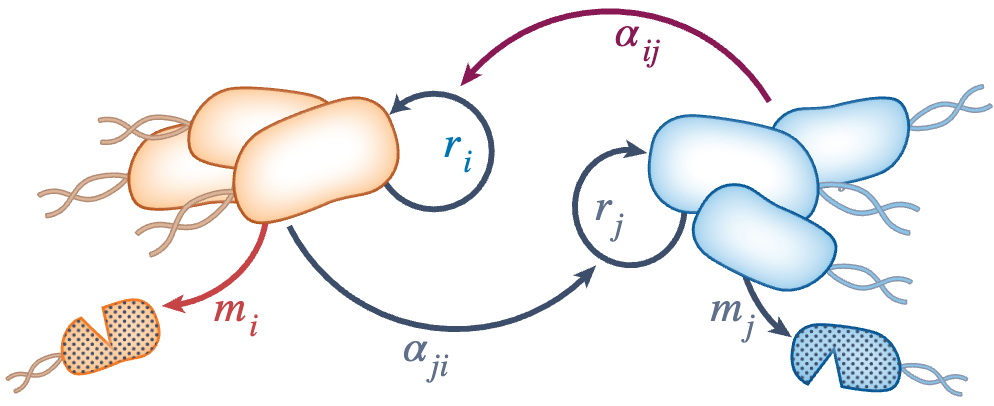
\includegraphics[width=\linewidth]{Figures/lotka_volterra_model.png}
        \caption{
            Lotka-Volterra model.
        }
        \label{fig:lotka_volterra_model}
    \end{subfigure}
    \hfill
    \begin{subfigure}{0.49\linewidth}
        \centering
        \captionsetup{width=1\linewidth}
        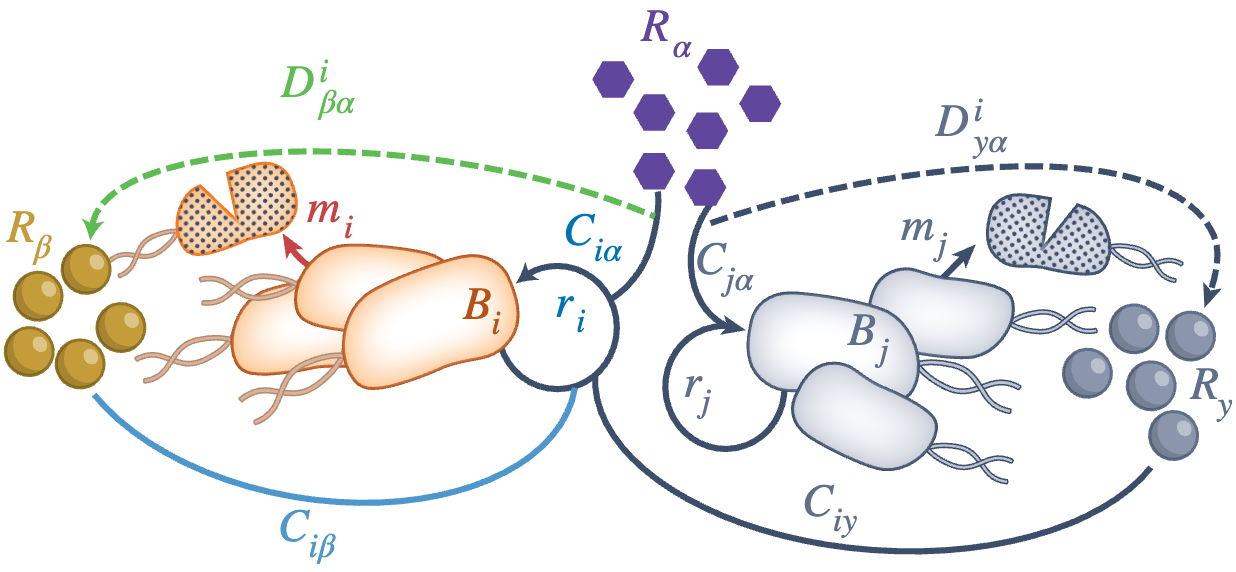
\includegraphics[width=\linewidth]{Figures/consumer_resource_model.png}
        \caption{
            Consumer Resource model.
        }
        \label{fig:consumer_resource_model}
    \end{subfigure}
    \caption{Different models and how the bacterial entities interact with itself, one another, resources and the environment. All figures sourced from \citet{vandenbergEcologicalModellingApproaches2022}}. 
\end{figure}


\section{Phage Biology}
\subsection{What Are Phages?}
Phages are small bundles of proteins that contain viral DNA. 
Phages are made up of multiple parts built like LEGO to complete the task of infecting a bacterium. 
\Cref{fig:figures:phage_diagram} shows the body parts of a phage. 
The aim of the phage is to find a suitable bacterial host and infect the host with viral DNA. 
The DNA alters the host's metabolic pathways to its benefit and hijacks the cellular replication process to create new copies of the phage. 
Eventually, the cell lyses, releasing the newly created phages into the environment to infect more bacteria. 
\begin{figure}[h!]
    \centering
    \begin{subfigure}{0.25\linewidth}
        \centering
        \captionsetup{width=1\linewidth}
        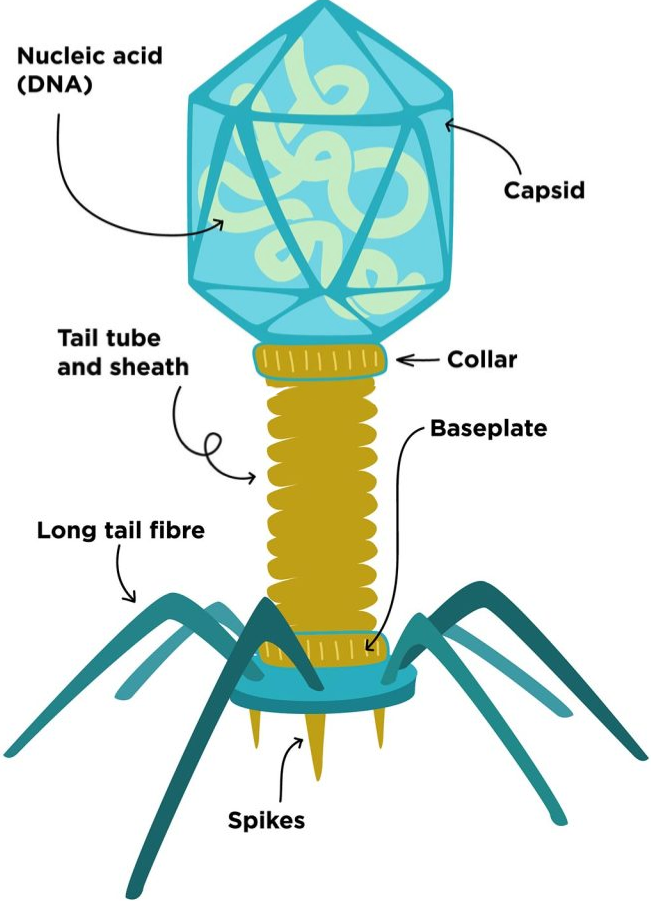
\includegraphics[width=\linewidth]{Figures/phage_diagram.png}
        \caption{
            Phage body structure. 
            % (https://www.newyorker.com/tech/annals-of-technology/phage-killer-viral-dark-matter). 
        }
        \label{fig:figures:phage_diagram}
    \end{subfigure}
    \hfill
    \begin{subfigure}{0.3\linewidth}
        \centering
        \captionsetup{width=1\linewidth}
        \includegraphics[width=\linewidth]{Figures/phage_real.png}
        \caption{
            Phages infecting an \textit{E. coli} bacteria. 
            % (https://www.newyorker.com/tech/annals-of-technology/phage-killer-viral-dark-matter). 
        }
        \label{fig:figures:phage_real}
    \end{subfigure}
    \hfill
    \begin{subfigure}{0.35\linewidth}
        \centering
        \captionsetup{width=1\linewidth}
        \includegraphics[width=\linewidth]{Figures/phage_impression.png}
        \caption{
            Artist representation of phages infecting a bacterium. 
            %(https://www.gettyimages.nl/detail/foto/bacteriophage-virus-attacking-a-bacterium-royalty-free-beeld/1179038792). 
        }
        \label{fig:figures:phage_impression}
    \end{subfigure}
    \caption{Parts of a phage, a real life picture of phages infecting an \textit{E. coli} bacterium, and an artist's impression of phages infecting a bacterium. }
\end{figure}

\subsection{How Does the Phage Cycle Work?}
There are 3 main parts to the phage-bacteria host cycle, the infection stage, the lysogenic cycle, and the lytic cycle. 
\Cref{fig:phage_life_cycle} shows a detailed overview of the phage cycle. 

In the infection stage, a phage attaches to the surface of a bacteria cell. 
The infection stage involves the phage searching for, detecting, and attaching to a bacterium, followed by DNA injection. 
Detection and attachment occur via phage receptor-binding proteins located at the tip of the phage tail that recognize specific receptors on the bacterial cell wall, triggering conformational changes that enable DNA injection. 
The success of this process depends on the specificity and density of both phage and bacterial receptors \cite{stoneUnderstandingExploitingPhage2019}. 
Once attached, the phage injects its DNA into the host cytoplasm, where it can replicate independently.
Once injected, the phage-cell pair can go into the lysogenic cycle or into the lytic cycle. 

The lysogenic cycle involves phage DNA integrating into the bacterial genome as a prophage, where it is replicated along with the host cell without causing immediate lysis.
The phage evades host defenses such as CBASS and CRISPR-Cas systems, which can start programmed cell death preventing phage replication or detect and degrade foreign DNA \cite{banhBacterialCGASSenses2023, levyCRISPRAdaptationBiases2015}. 
Programmed cell death helps recycle resources for other bacteria \cite{warwick-dugdaleHosthijackingPlanktonicPiracy2019}. 
Once integrated, the prophage can alter host fitness and provide resistance to other phages. 
During cell division, the prophage is copied into daughter cells but remains at risk of being excised by restriction enzymes \cite{sharpMolecularEvolutionBacteriophages1986}.
Under certain stress conditions, such as DNA damage or activation of the SOS response, the prophage can be induced to exit the genome and enter the lytic cycle \cite{waldorPhageRegulatoryCircuits2005, stoneUnderstandingExploitingPhage2019, fortierImportanceProphagesEvolution2013}.

The lytic cycle is the process where a phage infects a bacterium, hijacks its replication machinery to produce new phage components, assembles these parts, and ultimately lyses the host cell to release new phages. 
This involves hijacking the host's DNA replication to synthesize phage parts like the capsid, sheath, and tail \Cref{fig:figures:phage_diagram}. 
The phage does this by redirecting resources from internal cellular functions towards viral replication \cite{warwick-dugdaleHosthijackingPlanktonicPiracy2019}. 
The phage parts self-assemble via protein-protein and protein-nucleic acid interactions \cite{aksyukBacteriophageAssembly2011}. 
Phages induce bacterial lysis by producing holin proteins that disrupt the cell membrane, releasing the phages and resources \cite{wangHolinsProteinClocks2000}.

\section{Bacterial Defense Against Phages} 
\label{sec:literaturereview:bacterial_defense_against_phages}
There is a constant battle between phages and bacteria. 
The bacteria don't want to be killed by the phages, so they adapt defenses such as thickening of the cell wall or destroy the viral DNA. 

\subsection{Mutations in Bacterial DNA (Genetic (Co-)Evolution)}
As bacteria cells grow and divide, random point mutations can occur in the DNA. 
These mutations can affect phage defenses, like thickening the cell wall or removing a receptor, making it harder for the phages to detect and infect the cell. 
Mutations can be partially effective if full effectiveness requires multiple steps to achieve. 
Random mutations can also fail at making the bacteria more resistant to phages by increasing phage susceptibility or the mutation brings a cost to the bacteria cell by losing receptors on the cell wall \cite{lenskiTWOSTEPRESISTANCEESCHERICHIA1984}. 

\subsection{Horizontally Transferring DNA}
Bacteria can horizontally transfer DNA to other bacteria on contact. 
A donor cell can donate DNA fragments using a mechanism called a pilus. 
The pilus acts as a tunnel between the donor cell and the recipient cell so that DNA can be transferred from the donor cell to the receiver cell \cite{harbSsRNAPhagePenetration2020}. 

A phage can accidentally collect a piece of the host's DNA instead of its own DNA during assembly. 
The phage with the now dead hosts DNA can infect the next bacteria, injecting the new bacterium with the dead cell's DNA, horizontally transferring the DNA \cite{tamangHorizontalGeneTransfer2023, kasmanBacteriophages2025}. 
The transferred DNA can include natural phage defenses or significantly alter the genes and phenotype of the bacterium that future phages can't detect it anymore. 

\subsection{Phage Inactivation and Decoys}
Bacteria can further protect themselves by producing decoys that the phage will attach to instead of themselves. 
Freshly lysed bacteria may still have biomarkers that attract phages, leading phages to attach to non-viable cells where successful infection cannot occur.
Bacteria can also produce proteolytic enzymes that will damage the proteins found in a phage \cite{tanQuorumSensingDetermines2015}. 
Some bacteria can produce outer membrane vesicles that phages can absorb to, and later detach and float away with the phage \cite{rabinovitchBacterialDebrisEcological2003}. 
It is suspected that the impact of these vesicles acting as a sink is minor \cite{bullPhageBacterialDynamicsSpatial2018}. 

% \subsection{CRISPR-Cas Methods}
% CRISPR is a gene editing tool that cells can use to cut out specified/unwanted parts of a DNA strand. 
% Researchers are commonly using CRISPR to genetically engineer plants and animals to have specific features. 
% Strands of DNA can be selectively added or removed from a DNA strand to achieve a better, more desired DNA strand. 
% CRISPR defenses in the bacteria can detect the unwanted phage DNA and remove the DNA. 

\subsection{Phenotype Resistance}
Not all new phenotypes arise from genetic mutations. 
Resistance can result from phenotypic variation within a genetically identical population, allowing bacteria to express different resistance traits without altering their DNA.
\citet{guptaCombinatorialPhenotypicLandscape2025} found that some \textit{Bacteroides fragilis} bacteria were able to evade phage infection.  
The presence of combinatorial phenotypic states where differential expression of protective mechanisms created rare super-resistant cells capable of withstanding phage attack.
By acting together, these heterogeneously expressed anti-phage defense mechanisms created a phenotypic landscape where distinct protective combinations enabled the survival and re-growth of bacteria expressing these phenotypes without acquiring additional mutations. 

\subsection{Spatial Refuge/Biofilms} 
Usually bacteria and phages coexist in well mixed environments such as the ocean, however some environments offer natural structures for bacteria to hide behind. 
These structures can range from physical structure, like sediment in water to biochemical structures like biofilms, where the phages can't diffuse through the biofilm. 
In large enough quantities, bacteria and other microbial communities create biofilms, a layer of mucus containing various microbes. 
The thick mucus, microbes, and other spatial effects help protect the bacteria in the biofilm from external phages by making it hard for the phages to penetrate and diffuse through the mucus \cite{abedonPhageDelayEnhancing2017}. 
In the case of a lab experiment on an agar plate, bacteria protect one another by making it harder for the phages to diffuse through the system \cite{eriksenGrowingMicrocolonyCan2018}. 

Phage movement is passive, relying on diffusion through the environment or via pressure and temperature gradients \cite{lohrmannInfluenceBacterialSwimming2024}. 
Unlike phages, bacteria possess motility, allowing them to actively move through their environment increasing their chance of survival. 

\section{Phage Counter Defense Against Bacteria}
With some of the defenses that bacteria have developed, phages are always mutating to counter their defenses. 
If phages don't adapt to the ever-changing bacterial defenses, the phages will die out due to their inability to infect and multiply. 
It essentially becomes an arms race, seeing who can out-adapt the other. 
A delicate balance therefore needs to be achieved so that both the bacteria and the phages can coexist. 

\subsection{Genetic Mutations}
Mutations in viral DNA will affect how the phage body parts are designed and built. 
These mutations will affect external phage behavior such as how it detects a bacterium, as well as internal behavior such as evading detection and integrating with the cell's DNA. 
The changes will lead to changes in overall phage fitness, ie the ability for the phage to infect, replicate, and lyse bacteria. 

\subsection{Viral Recombination}
Multiple phages can infect a cell and replicate itself using the cells internal replication process. 
Each phage has its own building blocks. 
If the proteins that build the subparts of each phage have similar chemical properties, they can be swapped between phages \cite{aksyukBacteriophageAssembly2011}. 
This allows for biological diversity to spread throughout a phage population. 
Each phage body part can have unique characteristics such as better attachment rate, larger DNA storage capsule, or better probability of injection. 


\section{Phage Defense Against Phages}
Some phages can employ defenses against other phages from infecting the bacterial cell ensuring the host resources are all for itself. 
The act of preventing a secondary infection from a similar or closely related phage is called superinfection exclusion (SIE) \cite{patelAntiphageDefenceInhibition2024}. 
There are various methods of preventing further infections that are listed below. 

\subsection{Altering Cell Structure}
The prophage can alter the surface receptors of the bacteria, making it harder for other phages to detect the bacteria, reducing the chance of attachment and injection by other phages \cite{bucherPhageMachineSIEence2024}. 

\subsection{Protein Creation}
Other phages like the T4 phage can create proteins like the Spackle protein which inhibits the lysozyme activity used in the process of DNA injection by other phages \cite{bucherPhageMachineSIEence2024, kanamaruStructureFunctionT42020}. 
Some prophages can encode proteins that will interfere with the replication process of other phages. 
For example, the SieA protein encoded by phage P22 blocks infection from other phages \cite{leavittBacteriophageP22SieAmediated2024}. 

Tail Assembly Blocker (TAB) is an anti-phage defense mechanism encoded by a \textit{Pseudomonas aeruginosa} prophage. 
While TAB permits the invading phage to replicate its genome, it inhibits the assembly of the phage tail, thereby preventing the production of infectious virions. 
The prophage that encodes TAB is not affected by this inhibition, as it also expresses a protein that neutralizes TAB's blocking activity. 
Although the host cell still undergoes lysis, no infectious phages are released.

\subsection{Growth Curves Typically Seen in a Lab}
\label{sec:literaturereview:growth_curves_typically_seen_in_a_lab}

When choosing parameter values it is important to choose parameter values that could realistically be found in real life systems and be replicated in the lab. 
There are various features that a researcher will be looking for in growth curve produced in a lab.
A combination of these features results in an ideal growth curve that replicates real life bacterial growth. 

The idealized dynamics of bacterial populations undergoing phage infection have several phases. First, there is a clear exponential rise in bacteria growth, and can expect to grow 40-100x in the span of a few hours. 
At a certain point in time, the bacteria population start decreasing, almost as fast as they were growing. 

Phage populations also exhibit exponential growth, but with a delay in growth. 
There is initially no growth in phage population. 
After a set amount of time, the phage population will start to grow and peak a few hours after the bacteria population reached its peak. 
If there is no phage death or removal, the phage population will eventually reach a plateau when every bacteria has died. 

\Cref{fig:created:a_good_curve_linear} shows an example of a curve for a $1\times1\times1$ system that would typically be seen in a lab. 
\Cref{fig:created:a_good_curve_logarithmic} is the same plot but with a logarithmic y-axis. 
These specific plots exhibiting a clear growth, peak, delay, and death cycle. 

\begin{figure}[h!]
    \centering
    \begin{subfigure}{1\linewidth}
        \centering
        \captionsetup{width=1\linewidth}
        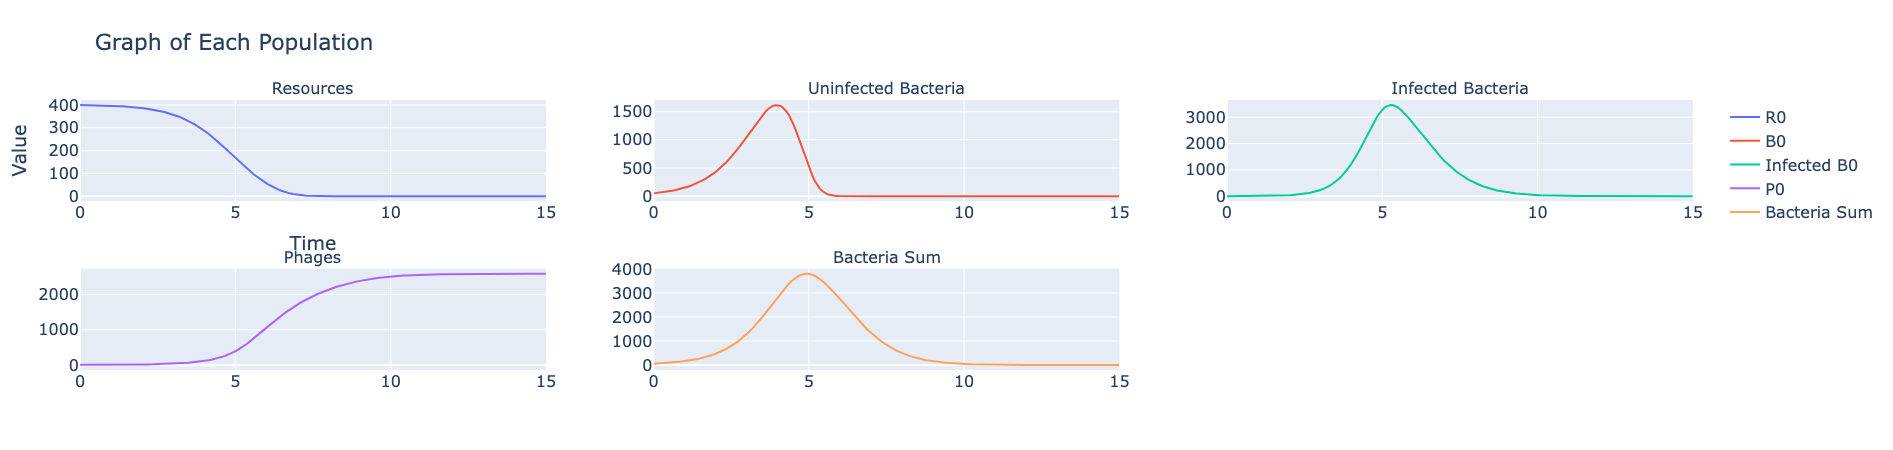
\includegraphics[width=\linewidth]{Plots/Created/a_good_curve_linear.png}
        \caption{
            An example linear y-axis for a curve that researchers aim to replicate. 
        }
        \label{fig:created:a_good_curve_linear}
    \end{subfigure}
    \hfill
    \begin{subfigure}{1\linewidth}
        \centering
        \captionsetup{width=1\linewidth}
        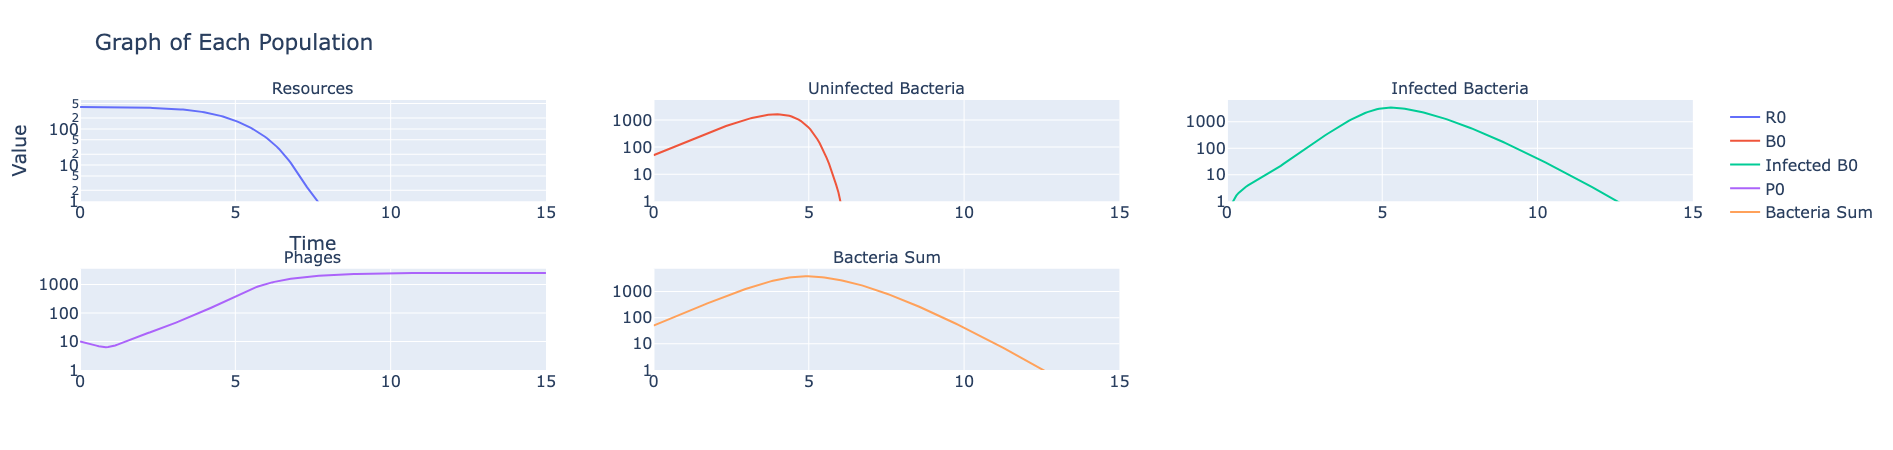
\includegraphics[width=\linewidth]{Plots/Created/a_good_curve_logarithmic.png}
        \caption{
            The equivalent logarithmic y-axis plot for a curve that researchers aim to replicate. 
        }
        \label{fig:created:a_good_curve_logarithmic}
    \end{subfigure}
    \caption{
        Growth population of a $1\times1\times1$ system. 
        The log plot allows to see behavior happening at values approaching and to plot data on a logarithmic scale. 
        The parameters used for this plot can be found in \Cref{tab:appendixE:a_good_curve}. 
    }
    \label{fig:created:a_good_curve}
\end{figure}

\section{Bacteria and Phages in the Lab}
Researchers around the world are running lab experiments to gain further knowledge of the interactions between phages and bacteria. 
The aim is to better understand how phages work and interact with bacteria at a molecular, host, and population level. 

\subsection{Running Experiments}
A researcher might run the experiment in a liquid medium containing water, carbon and nitrogen sources, and other chemicals such as anti-foaming or pH control chemicals. 
This liquid medium, often referred to as broth, allows for the cultivation of bacteria in a well-mixed environment, enabling researchers to monitor bacterial growth and phage infection dynamics over time. 
By adjusting parameters such as resource concentration, temperature, agitation speed, and pH, researchers can simulate different environmental conditions and observe their effects on phage-bacteria interactions. 

Samples can be taken at various time points to measure bacterial density, phage titer, and resource concentration, providing quantitative data for model validation and hypothesis testing. 
The researcher received an ODE-like curve of the bacteria density. 
Researchers can create a mathematical interpretation of the bacteria growth curve and run curve fitting algorithms to find the bacteria's growth rate. 
The phage parameters such as latent time and burst size can be found by analyzing the phage one-step growth curve \cite{gengUsingBacterialPopulation2024, mullaExtremeDiversityPhage2024}. 

\subsection{Chemostats}
Commonly used setups include liquids containing phages, bacteria, and resources in a chemostat and batch culture. 
Chemostats allow for continuous addition of resources and removal of waste, maintaining steady-state conditions ideal for studying long-term dynamics.
Bacteria density in clear liquid mediums can be measured optically using light. 
As the bacteria grow and die, the solution will get more cloudy. 
By shining a light through a vial with bacteria growth, the change in light refraction and intensity can be measured. 
A researcher might also be interested in using a mass spectrometer to measure the density of phages and resources at specific time points. 

\subsection{Petri Dishes}
Petri dishes are another commonly used way to grow bacterial colonies. 
Agar, a jelly-like substance derived from seaweed, is commonly used as a solid growth medium in petri dishes. 
Agar provides a stable surface for bacteria to grow on and form visible colonies. 
When phages are introduced, clear zones called plaques appear where phages have infected and lysed the bacteria, allowing for quantification and observation of phage activity. 
The phages can diffuse on the agar plate, infecting neighboring cells. 
Phage infection creates clear plaques (2-3 mm) where bacteria are absent. 
\Cref{fig:phage_petri_dish} shows an example of a bacteria lawn with phage plaques. 

\subsection{Measuring Growth}
Bacteria density in clear liquid mediums can be measured optically using light. 
As the bacteria grow and die, the solution will get more cloudy. 
By shining a light through a vial with bacteria growth, the change in light refraction and intensity can be measured. 
A researcher might also be interested in using a mass spectrometer to measure the density of phages and resources at specific time points. 

With petri dishes, it is harder to measure the bacterial growth. 
It might be possible to wash the bacteria off into a test tube with water to measure the optical density (OD), but the results are inconsistent. 
Even though using a special spectrophotometer allows consistent results, the results are dependent on the medium, the length of travel through the medium, bacteria size, and density. 
The device also has to be calibrated to ensure proper results, and results cant be compared across devices without calibration \cite{bealRobustEstimationBacterial2020}. 
Changing methods to using $\frac{\textit{cells}}{\textit{ml}}$ instead of OD can be used to directly compare results across experiments, labs, and bacteria colonies \cite{miraEstimatingMicrobialPopulation2022}. 

It might be possible to quantify the change in plaque size, either by hand or using an image analysis program, but the results might be inaccurate and sensitive to different lighting conditions. 

\begin{figure}[h!]
    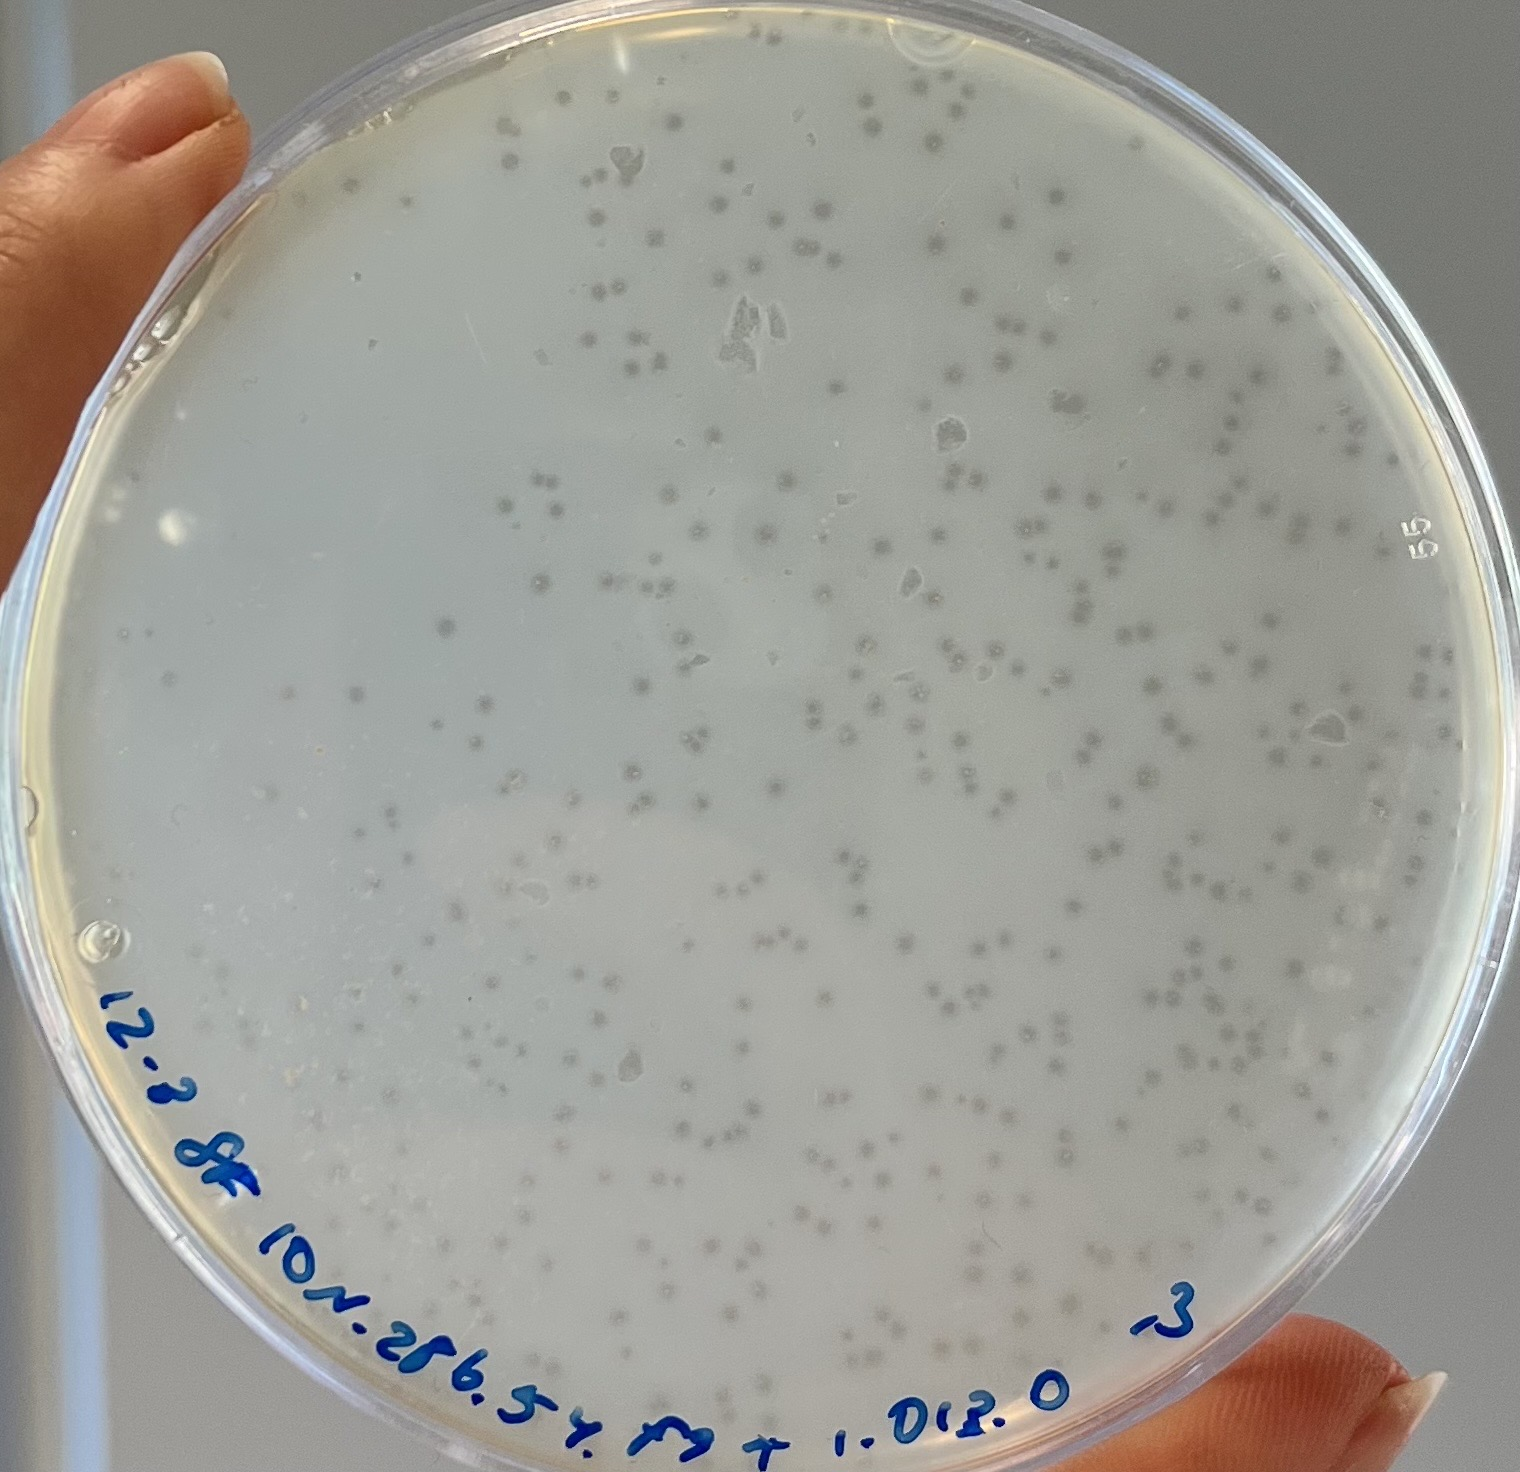
\includegraphics[width=0.5\textwidth]{Figures/phage_petri_dish.jpeg}
    \centering
    \caption{
        Bacteria lawn, the dots on the petri dish show no bacteria growth due to the presence of phages. 
        Photo courtesy of S. Flickinger. 
    }
    \label{fig:phage_petri_dish}
\end{figure}
\subsection{Serial Transfer}
Serial transfer (ST) is a method employed by bacteriologist where after a set amount of time, the bacteriologist pipettes medium containing phages, bacteria, and resources out of a test tube and adds the old media into a new test tube with new media.
At this stage, the bacteriologist can add more bacteria or phages to the test tube. 
However, usually only resources are added during the transfer process.
Researchers can optically measure the bacteria density using an optical density machine or employ a mass spectrometer to determine the phage concentration at set time points during the experiment. 
As the bacteria grow, they consume the resources found in the medium.
The resources will eventually run out, and the bacteria die out due to a lack of resources.
By introducing new resources at set time intervals, the bacteria can regrow and exhibit a semi-stationary behavior.

\subsection{Growth Curves Typically Seen in a Lab}
\label{sec:literaturereview:growth_curves_typically_seen_in_a_lab}

When choosing parameter values it is important to choose parameter values that could realistically be found in real life systems and be replicated in the lab. 
There are various features that a researcher will be looking for in growth curve produced in a lab.
A combination of these features results in an ideal growth curve that replicates real life bacterial growth. 

The idealized dynamics of bacterial populations undergoing phage infection have several phases. First, there is a clear exponential rise in bacteria growth, and can expect to grow 40-100x in the span of a few hours. 
At a certain point in time, the bacteria population start decreasing, almost as fast as they were growing. 

Phage populations also exhibit exponential growth, but with a delay in growth. 
There is initially no growth in phage population. 
After a set amount of time, the phage population will start to grow and peak a few hours after the bacteria population reached its peak. 
If there is no phage death or removal, the phage population will eventually reach a plateau when every bacteria has died. 

\Cref{fig:created:a_good_curve_linear} shows an example of a curve for a $1\times1\times1$ system that would typically be seen in a lab. 
\Cref{fig:created:a_good_curve_logarithmic} is the same plot but with a logarithmic y-axis. 
These specific plots exhibiting a clear growth, peak, delay, and death cycle. 

\begin{figure}[h!]
    \centering
    \begin{subfigure}{1\linewidth}
        \centering
        \captionsetup{width=1\linewidth}
        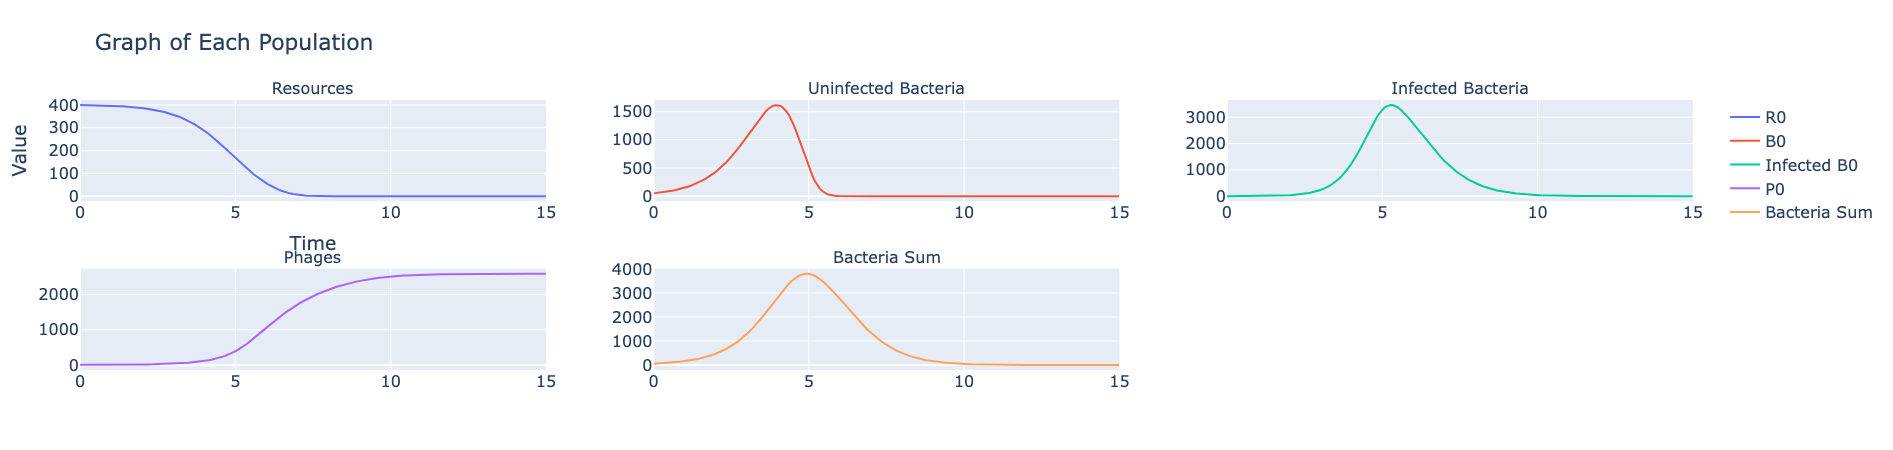
\includegraphics[width=\linewidth]{Plots/Created/a_good_curve_linear.png}
        \caption{
            An example linear y-axis for a curve that researchers aim to replicate. 
        }
        \label{fig:created:a_good_curve_linear}
    \end{subfigure}
    \hfill
    \begin{subfigure}{1\linewidth}
        \centering
        \captionsetup{width=1\linewidth}
        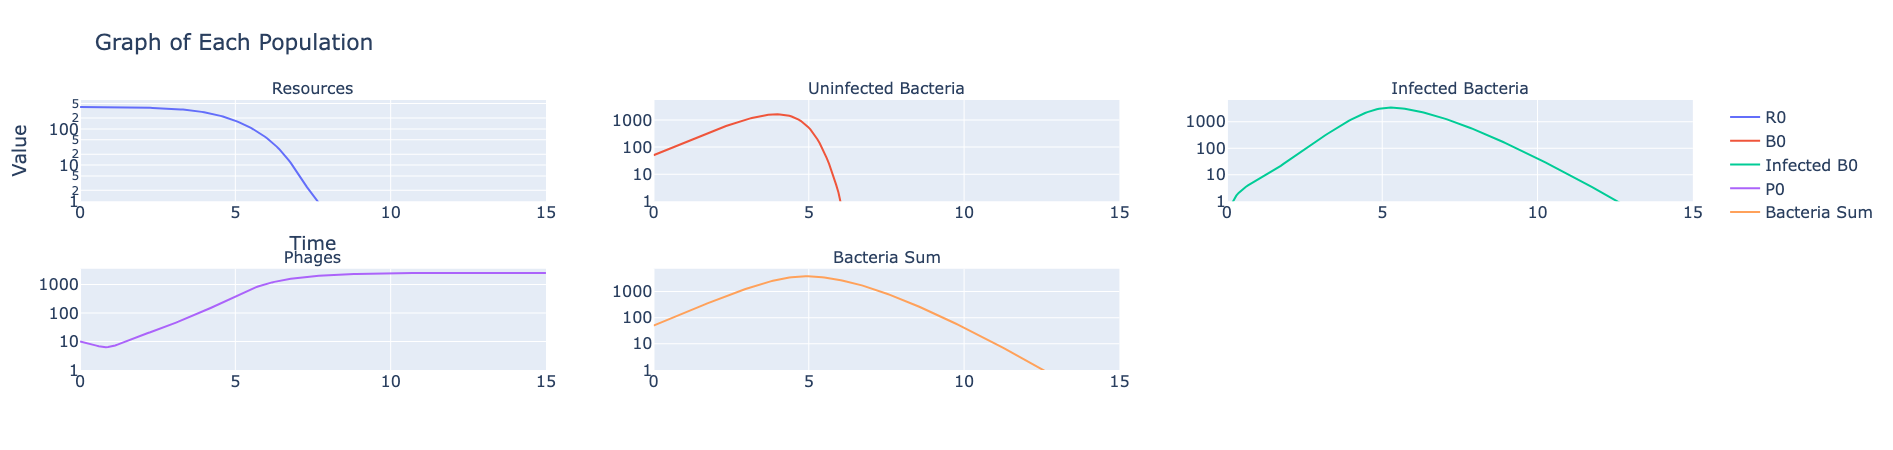
\includegraphics[width=\linewidth]{Plots/Created/a_good_curve_logarithmic.png}
        \caption{
            The equivalent logarithmic y-axis plot for a curve that researchers aim to replicate. 
        }
        \label{fig:created:a_good_curve_logarithmic}
    \end{subfigure}
    \caption{
        Growth population of a $1\times1\times1$ system. 
        The log plot allows to see behavior happening at values approaching and to plot data on a logarithmic scale. 
        The parameters used for this plot can be found in \Cref{tab:appendixE:a_good_curve}. 
    }
    \label{fig:created:a_good_curve}
\end{figure}

\section{Software Mathematically Modelling Phages, Bacteria, and Resources}
Some software programs modelling phage-bacteria-resource interactions already exists. 
\subsection{Cocktail}
\citet{nilssonCocktailComputerProgram2022} developed Cocktail to model phage-bacteria-resource kinetics in a chemostat. 
The model assumes there is one bacteria strain that can be infected by phage A and phage B, and by both phages at the same time, phage AB. 
The model models bacterial resistance to phage A, B, and AB. 
The user can control the parameter values such as resistance rate to A, B, and AB, resource concentration and outflow, and phage adsorption rate. 
The user can also control model settings, such as if the model is deterministic or stochastic, and the step size \cite{nilssonCocktailComputerProgram2022}. 
Four sample output plots are shown in \Cref{fig:sourced:cocktail_plot}. 

\subsection{PhageDyn}
PhageDyn is a Java applet that models phage dynamics in multi-reactor industrial wastewater treatment plant models. 
PhageDyn interacts with existing GPS-X \cite{AdvancedWastewaterModelling} files to incorporate phage dynamics into models of industrial wastewater treatment plants \cite{krysiak-baltynSimulationPhageDynamics2017}. 
\citet{krysiak-baltynSimulationPhageDynamics2017} developed PhageDyn to determine how phages can reduce foaming caused by bacteria in wastewater treatment plants, another real life application of phages \cite{heardEffectFilamentousBacteria2008}. 
PhageDyn does not simulate phage dynamics on its own but rather manipulates existing files in GPS-X in order to incorporate phage dynamics in wastewater treatment plant models. 
\Cref{fig:sourced:phagedyn_plot} shows the output that PhageDyn provides. 

\subsection{Cocktail and PhageDyn Limitations}
\label{sec:literature:cocktail_and_phagedyn_limitations}
There are limitations to Cocktail and PhageDyn. 
Cocktail can model up to a $2\times 1 \times 1$ system, and is designed to model a chemostat. 
Chemostats receive a constant influx of new resources and a constant removal of medium from the chemostat. 
Cocktail's model can not be easily adapted to other models. 
The ODE model accepts inputs from a hardcoded GUI frontend. 
So any changes to the frontend or to the ODE model will require changes to the ODE model and the frontend to accept the new inputs and outputs. 
The code for Cocktail is open source, so adding new buttons and changing the model should not pose a significant challenge, but still an undertaking. 

PhageDyn works with GPS-X, a very niche wastewater treatment modelling software. 
PhageDyn is programmed for a very specific task with no flexibility in changing the model or inputs. 
PhageDyn assumes biomass, instead of individual bacteria populations. 
However, PhageDyn is no longer available for download.

\begin{figure}
    \centering
    \begin{subfigure}{0.49\linewidth}
        \centering
        \captionsetup{width=1\linewidth}
        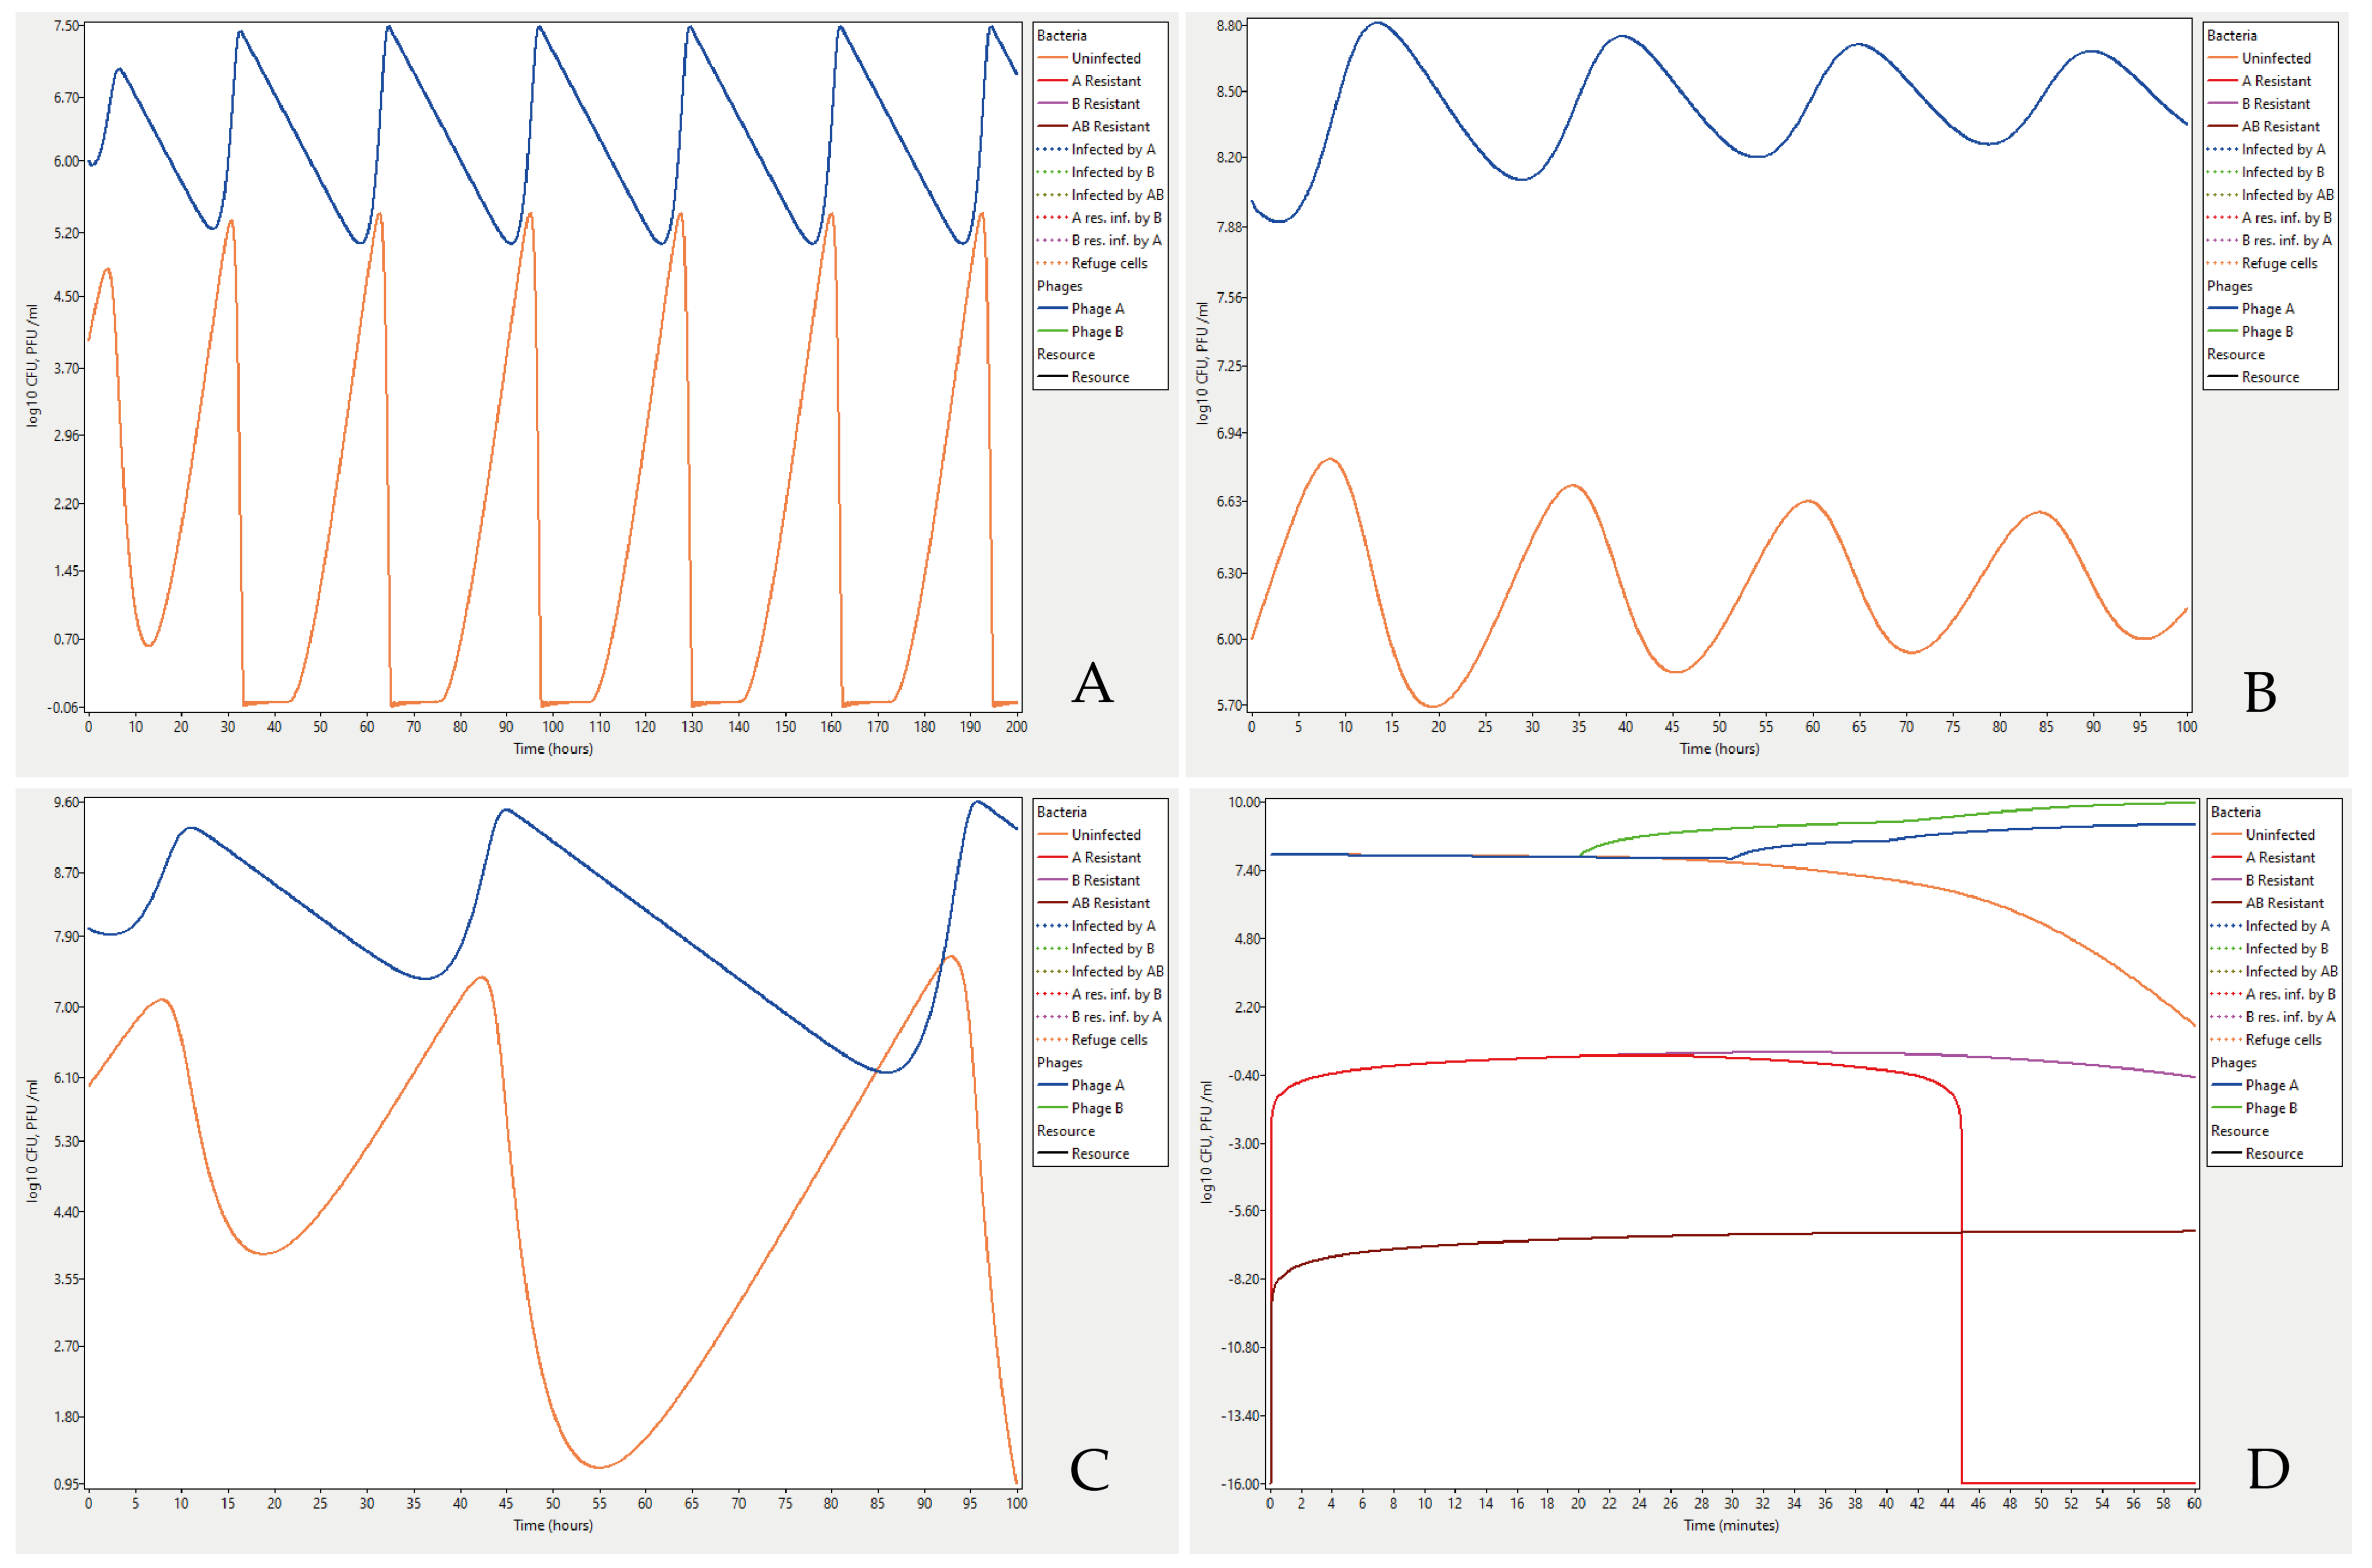
\includegraphics[width=\linewidth]{Plots/Sourced/cocktail_plot.png}
        \caption{
            Figure A) \textit{E. coli} infected with phage T4 in a chemostat exhibiting an oscillating growth behavior, following the model of \citet{bohannanEffectResourceEnrichment1997}. 
            Figure B) Oscillations of bacteria and phages can exist at higher titers, dependent on low resource concentration, following the model of \citet{lenskiDynamicsInteractionsBacteria1988}. 
            Figure C) As the concentration of resources change, this results in increasing oscillations, but not going extinct. 
            Figure D) A system modelling the interactions with phage A and B. 
        }
        \label{fig:sourced:cocktail_plot}
    \end{subfigure}
    \hfill
    \begin{subfigure}{0.49\linewidth}
        \centering
        \captionsetup{width=1\linewidth}
        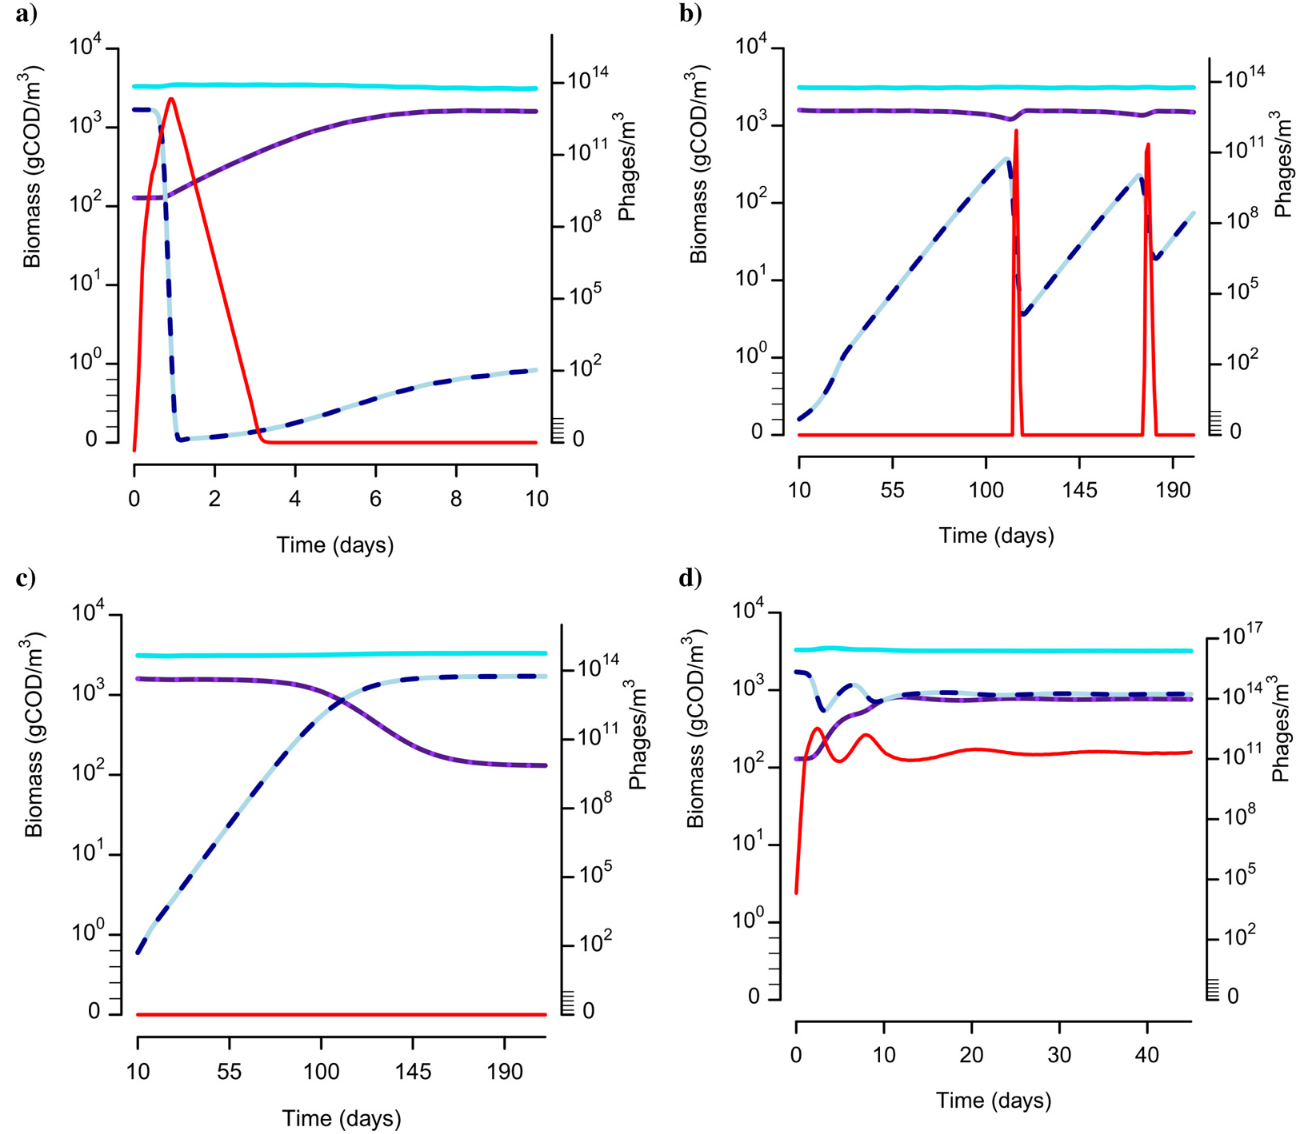
\includegraphics[width=\linewidth]{Plots/Sourced/phagedyn_plot.png}
        \caption{
            \textcolor[HTML]{551A8C}{\textbf{Purple}} is heterotrophic biomass, 
            \textcolor[HTML]{4580B4}{\textbf{Blue}} is foaming biomass, 
            \textcolor[HTML]{FF0000}{\textbf{Red}} is phages, 
            \textcolor[HTML]{01E6EE}{\textbf{Light Blue}} is total suspended solids. 
            Figure A) Biomass concentration immediately post phage dosing. 
            Figure B) Biomass concentration with low phage concentration and maintain low concentration post spike in population count. 
            Figure C) Biomass concentration when phages are extinct. 
            Figure D) Biomass concentration with a less virulent and low adsorption rate phage, co-existence with biomass reached. 
            A change in phage concentration shows a decrease in heterotrophic and foaming biomass \cite{krysiak-baltynSimulationPhageDynamics2017}. 
        }
        \label{fig:sourced:phagedyn_plot}
    \end{subfigure}
    \caption{Example output from Cocktail and PhageDyn respectively. For PhageDyn, concentration of heterotrophic biomass in an aerobic plug flow across four situations.
        See \citet{nilssonCocktailComputerProgram2022} and \citet{krysiak-baltynSimulationPhageDynamics2017} for more information on parameter values and supplementary resources. 
    }
    \label{fig:sourced:cocktail_and_phagedyn}
\end{figure}

\section{The Golding Model}
\label{sec:golding_model}
The default model that will be used in this thesis, the “Golding model“, sourced from \citet{gengUsingBacterialPopulation2024}, describes the interactions between resources, uninfected bacteria, infected bacteria, and phages. 

\subsection{The Original Golding Model}
The model describes three biological processes, cell consumption of resources and growing, phage/cell encounters and infection, and cell lysis. 
The cell growth process is described by $g(R, v, K)$, the instantaneous growth rate dependent on the Monod equation, where $v$ is the maximal growth rate of the bacteria population and $K$ is the Monod constant. 
Bacteria consume a resource with rate $e$. 

Once infected by a phage, the bacteria goes from $U$ to $I_1$. 
The bacteria goes through $M$ stages of infection $I_1, \dots, I_M$ before lysing, 
The bacteria goes from state $I_k$ to state $I_{k+1}$ with equal transition rate $\frac{M}{\tau}$. 
The infection rate of a cell is $r$. 
After a bacteria lyses after stage $I_M$, $\beta$ phages are released, the burst size of the phage. 

\begin{eqfloat}[ht!]
    \begin{align}
        \frac{dR}{dt} &= -e \cdot g(R, v, K)\cdot (U + \sum_{k=1}^{M} I_k)\\
        \frac{dU}{dt} &= g(R, v, K)\cdot U - r\cdot U \cdot P\\
        \frac{dI_1}{dt} &= r\cdot U \cdot P - \frac{M}{\tau}\cdot I_1\\
        \frac{dI_k}{dt} &= \frac{M}{\tau}(I_{k-1}-I_k) \text{ for } k=2, \dots, M \\
        \frac{dP}{dt} &= \beta \cdot\frac{M}{\tau} \cdot I_M - r\cdot(U + \sum_{k=1}^{M} I_k)\cdot P \\
        g(R, v, K) &= \frac{v\cdot R}{R + K}
        \label{eq:golding_model}
    \end{align}
    \caption{
        The Golding model sourced from \citet{gengUsingBacterialPopulation2024}. 
        The text in \textcolor{red}{red} has been added to the model, adding (the wash-in) fresh resources ($\omega^i$) and the removal (wash-out) of entities ($\omega^o$). 
        The washin is not dependent on the current resource population, as it is a constant rate being added. 
        By default these values are 0.
        A summary of the parameters can be found at \Cref{tab:appendixA:parameter_table_simple_golding_model}. 
    }
\end{eqfloat}

\subsection{The Adapted Golding Model}
\label{sec:adapted_golding_model}
The original Golding model is specifically designed for a $1\times 1 \times 1$ system. 
In order to adapt this model to fit an $p \times b \times r$ model, the model needs to be slightly adapted. 
There are other changes that can be made to the model, for example by adding a washin rate $\omega^{i}$, where resources are constantly being introduced, and a washout rate $\omega^{o}$ where all entities are washed out at a constant rate. 
These changes are highlighted in \Cref{eq:adapted_golding_model} in \textcolor{red}{red}. 

The adapted model accounts for the interactions of multiple phages, bacteria, and resources, and assumes the interactions occur independently of one another. 

\begin{eqfloat}
    \begin{align}
        \frac{dR_r}{dt} &= -\sum_{b \in B} e_{b r} \cdot g(R_r, v_{b r}, K_{b r})\cdot (U_b + \sum_{k=1}^{M} I_{b_k}) \mathcolor{red}{+ w^i -w^o \cdot R_r}\\
        \frac{dU_b}{dt} &= U_b \cdot \sum_{r \in R} g(R_r, v_{b r}, K_{b r}) - U_b \cdot \sum_{p \in P} r_{p b} \cdot P_p -\mathcolor{red}{-w^o \cdot U_b}\\
        \frac{dI_{b_1}}{dt} &= U_b \cdot \sum_{p \in P}r_{p b} \cdot P_p - \frac{M}{\tau_b}\cdot I_{b_1} \mathcolor{red}{-w^o \cdot I_{b_1}}\\
        \frac{dI_{b_k}}{dt} &= \frac{M}{\tau_b}(I_{b_{k-1}}-I_{b_k}) \mathcolor{red}{-w^o \cdot I_{b_k}}\text{ for } k=2, \dots, M \\
        \frac{dP_p}{dt} &= \sum_{b\in B}\beta_{p b}\cdot\frac{M}{\tau_b} \cdot I_{b_M} - r_{p b}\cdot(U_b + \sum_{k=1}^{M} I_{b_k})\cdot P_p \mathcolor{red}{-w^o \cdot P_p}\\
        g(R_r, v_{b r}, K_{b r}) &= \frac{v_{b r} \cdot R_r}{R_r + K_{b r}}
        \label{eq:adapted_golding_model}
    \end{align} 
    \caption{
        The adapted Golding model. 
        The probability of phage $p$ infecting bacteria $b$ is $r_{p b}$ is not to be confused with the resource concentration $R_r$. 
        The interactions are a sum of all interactions due to all interactions taking place at the same time. 
    }
\end{eqfloat} %Related literature and material (8-12 pages)
\lhead{\emph{Methods}}
\chapter{Methods}
\label{Methods}
\section{Project Overview}
To help complete this Master thesis, I created various tools that would help create the final model outputs.
The project is divided into four parts. 
The first part is the tool that a user can use to design and create the network of agent interactions. 
The second part is the simulation framework that handles the data and runs the ODE solving method. 
The third part is a dashboard that runs in the browser. The dashboard allows for a user to interact with the model, for example by changing parameter and environment values, and run some basic simulations and receive different plots as output. 
The final part allows the user to download the simulation data to create their own custom graphs and analyses. 

A flowchart showing the user-system interactions can be seen in \nameref{AppendixC}. 

\section{The Golden Model}
\label{sec:golden_model}
In this report, the default model, called the “Golden model“ \cite{gengUsingBacterialPopulation2024} that will be used for all simulations is as follows:

% \begin{equ}[!ht]
%     \begin{equation}
%         \frac{dR}{dt} &= -e \cdot g(R, v, K)\cdot (U + \sum_{i=1}^{M} I_M) \mathcolor{red}{+ w^i -w^o \cdot R}\\
%         \frac{dU}{dt} &= g(R, v, K)\cdot U - r\cdot U \cdot P \mathcolor{red}{-w^o \cdot U}\\
%         \frac{dI_1}{dt} &= r\cdot U \cdot P - \frac{M}{\tau}\cdot I_1 \mathcolor{red}{-w^o \cdot I_1}\\
%         \frac{dI_k}{dt} &= \frac{M}{\tau}(I_{k-1}-I_k) \mathcolor{red}{-w^o \cdot I_k}\text{ for } k=2, \dots, M \\
%         \frac{dP}{dt} &= \beta \cdot\frac{M}{\tau} \cdot I_M - r\cdot(U + \sum_{i=1}^{M} I_M)\cdot P \mathcolor{red}{-w^o \cdot P} \\
%         g(R, v, K) &= \frac{v\cdot R}{R + K}
%     \end{equation}
%     \caption{Caption of the equation}
% \end{equ} 

\begin{eqfloat}
    \begin{align}
        \frac{dR}{dt} &= -e \cdot g(R, v, K)\cdot (U + \sum_{i=1}^{M} I_M) \mathcolor{red}{+ w^i -w^o \cdot R}\\
        \frac{dU}{dt} &= g(R, v, K)\cdot U - r\cdot U \cdot P \mathcolor{red}{-w^o \cdot U}\\
        \frac{dI_1}{dt} &= r\cdot U \cdot P - \frac{M}{\tau}\cdot I_1 \mathcolor{red}{-w^o \cdot I_1}\\
        \frac{dI_k}{dt} &= \frac{M}{\tau}(I_{k-1}-I_k) \mathcolor{red}{-w^o \cdot I_k}\text{ for } k=2, \dots, M \\
        \frac{dP}{dt} &= \beta \cdot\frac{M}{\tau} \cdot I_M - r\cdot(U + \sum_{i=1}^{M} I_M)\cdot P \mathcolor{red}{-w^o \cdot P} \\
        g(R, v, K) &= \frac{v\cdot R}{R + K}
        \label{eq:golden_model}
    \end{align}
    \caption{
        The golden model taken from \citet{gengUsingBacterialPopulation2024}. 
        The text in red has been added to model adding (the wash-in) fresh resources ($\omega^i$) 
        and the removal (wash-out) of agents $\omega^o$. By default these values are 0.
        A summary of the parameter meanings can be found at \Cref{tab:parameter_table_simple_golden_model}. 
    }
\end{eqfloat}

where $R$ is resources, $U$ is uninfected bacteria, $I_{1, \dots, M}$ is the infected stage of the bacteria, and $P$ is the phage population. 

The model describes three biological processes, cell consumption of resources and growing, phage/cell encounters and infection, and cell lysis. 
The cell growth process is described by $g(R, v, K)$, the instantaneous growth rate dependent on the Monod equation, where $v$ is the maximal growth rate and $K$ is the Monod constant. 
The consumption rate of a resource by a bacteria is $e$. 

Once infected by a phage, the bacteria goes from $U$ to $I_1$. 
The bacteria goes through $M$ stages of infection $I_1, \dots, I_M$ before lysing, where the bacteria goes from state $I_k$ to state $I_{k+1}$ with equal transition rate $\frac{M}{\tau}$. The probability of a successful infection of a cell is $r$. 
After a bacteria lyses after stage $I_M$, $\beta$ phages are released, the burst size of the phage. 

However this model is specifically designed for a $1\times 1 \times 1$ model. 
In order to adapt this model to fit an $p \times b \times r$ model, the model needs to be slightly adapted. 
There are other changes that can be made, to the model, for example by adding a washin rate $\omega^{i}$, where resources are constantly being introduced, and a washout rate $\omega^{o}$ where all agents are washed out at a constant rate. 

\subsection{The Adapted Golden Model}
\label{sec:adapted_golden_model}
The adapted model accounts for the interactions of multiple agents. 
\begin{eqfloat}
    \begin{align}
        \frac{dR_r}{dt} &= -\sum_{b \in B} e_{b, r} \cdot g(R_r, v_{b, r}, K_{b, r})\cdot (U_b + \sum_{i=1}^{M} I_{i_b}) + w^i_r - w^o \cdot R_r\\
        \frac{dU_b}{dt} &= U_b \cdot \sum_{r \in R} g(R_r, v_{b, r}, K_{b, r}) - U_b \cdot \sum_{p \in P} r_{p, b} \cdot P_p - w^o \cdot U_b\\
        \frac{dI_{b_1}}{dt} &= U_b \cdot \sum_{p \in P}r_{p, b} \cdot P_p - \frac{M}{\tau_b}\cdot I_{b_1} - w^o \cdot I_{b_1}\\
        \frac{dI_{b_k}}{dt} &= \frac{M}{\tau_b}(I_{b_{k-1}}-I_{b_k}) - w^o \cdot I_{b_k}\text{ for } k=2, \dots, M \\
        \frac{dP_p}{dt} &= \sum_{b\in B}\beta_{p, b}\cdot\frac{M}{\tau_b} \cdot I_{b_M} - r_{p, b}\cdot(U_b + \sum_{i=1}^{M} I_{b_i})\cdot P_p - w^o \cdot P_p\\
        g(R_r, v_{b, r}, K_{b, r}) &= \frac{v_{b, r} \cdot R_r}{R_r + K_{b, r}}
        \label{eq:adapted_golden_model}
    \end{align}. 
    \caption{
        Probability of phage infection $r_{p, b}$ is not to be confused with $R_r$, short for Resource $r$. 
        The interactions are a sum of all interactions due to all interactions taking place at the same time. 
    }
\end{eqfloat}

\subsection{Network Creation Tool}
\label{sec:network_creation_tool}
The network creation tool is the first step that a user needs to use, and it revolves around using a GUI tool built to create and edit the graph representation of the agent interaction.
Numerous interactions occur between agents in a microbial environment.
However, not every agent can and will interact with one another.
Based on which agents interact with one another, a network topography representing the agent interactions and dynamics can be created. 

Every node represents a unique agent, and each agent has their own intrinsic properties. 
The user can intuitively define agents, their interactions, environmental and model settings using the GUI tool. 
This tool allows users to quickly and intuitively define agents and their attributes, agent interactions and their attributes, environmental data, and model settings.
An edge links two agents together if there is an arbitrary interaction occurring between the agents, with the properties exhibited in the interaction dependent on the interacting agents. 
Self interactions are allowed in the network. 
There is an environment node that is used to store global environmental data, such as the temperature and pH of the system.
The settings node holds information such as simulation length, max time step, and the type of ODE solver to use.
The tool provides functionalities for adding, editing, and visualizing nodes and edges, as well as importing and exporting the network structure.  

Once the user is happy with the graph shape, they can export the network representation for use in \nameref{sec:simulation_framework}, \nameref{sec:visualization_framework}, and \nameref{sec:custom_visualizations_and_framework}. 
The most important part is that the user defines the shape and the attributes of the network, as that can't be edited in part 2 onwards. 
It is possible go back to the network creation tool and upload the graph to the tool to be able to edit the network representation. \newline
The user can edit the values of the attributes in \nameref{sec:visualization_framework}, so the parameter values do not have to be perfect. 
As such, the user does not need to keep on using the GUI tool to edit parameter values. 

\Cref{fig:ss:initial_startup_GUI_tool} shows the layout of the GUI tool. \Cref{fig:ss:example_network} shows an example network that can be created.
There are numerous buttons that can be used to edit the graph, for example adding or removing nodes and edges. 
By default, an environment node holding parameters such as pH and temperature is added.
A settings node is added as well, holding settings data to be used for the solver, like the type of solver or simulation length.
Manually adding nodes and edges can get tedious and repetitive for large graphs, so the user can add multiple nodes and edges at the same time.
Nothing can interact with the environment and setting node, as they are used to hold data about the environment and network solver.
The user can alter the default attribute name and value by importing the GUI tool class and overriding the method implementation implementing the default names and values. 
The user can self-decide which parameter values to give, and if and how the parameter values are randomized. 

\begin{figure}
    \centering
    \begin{subfigure}{0.49\linewidth}
        \centering
        \captionsetup{width=1\linewidth}
        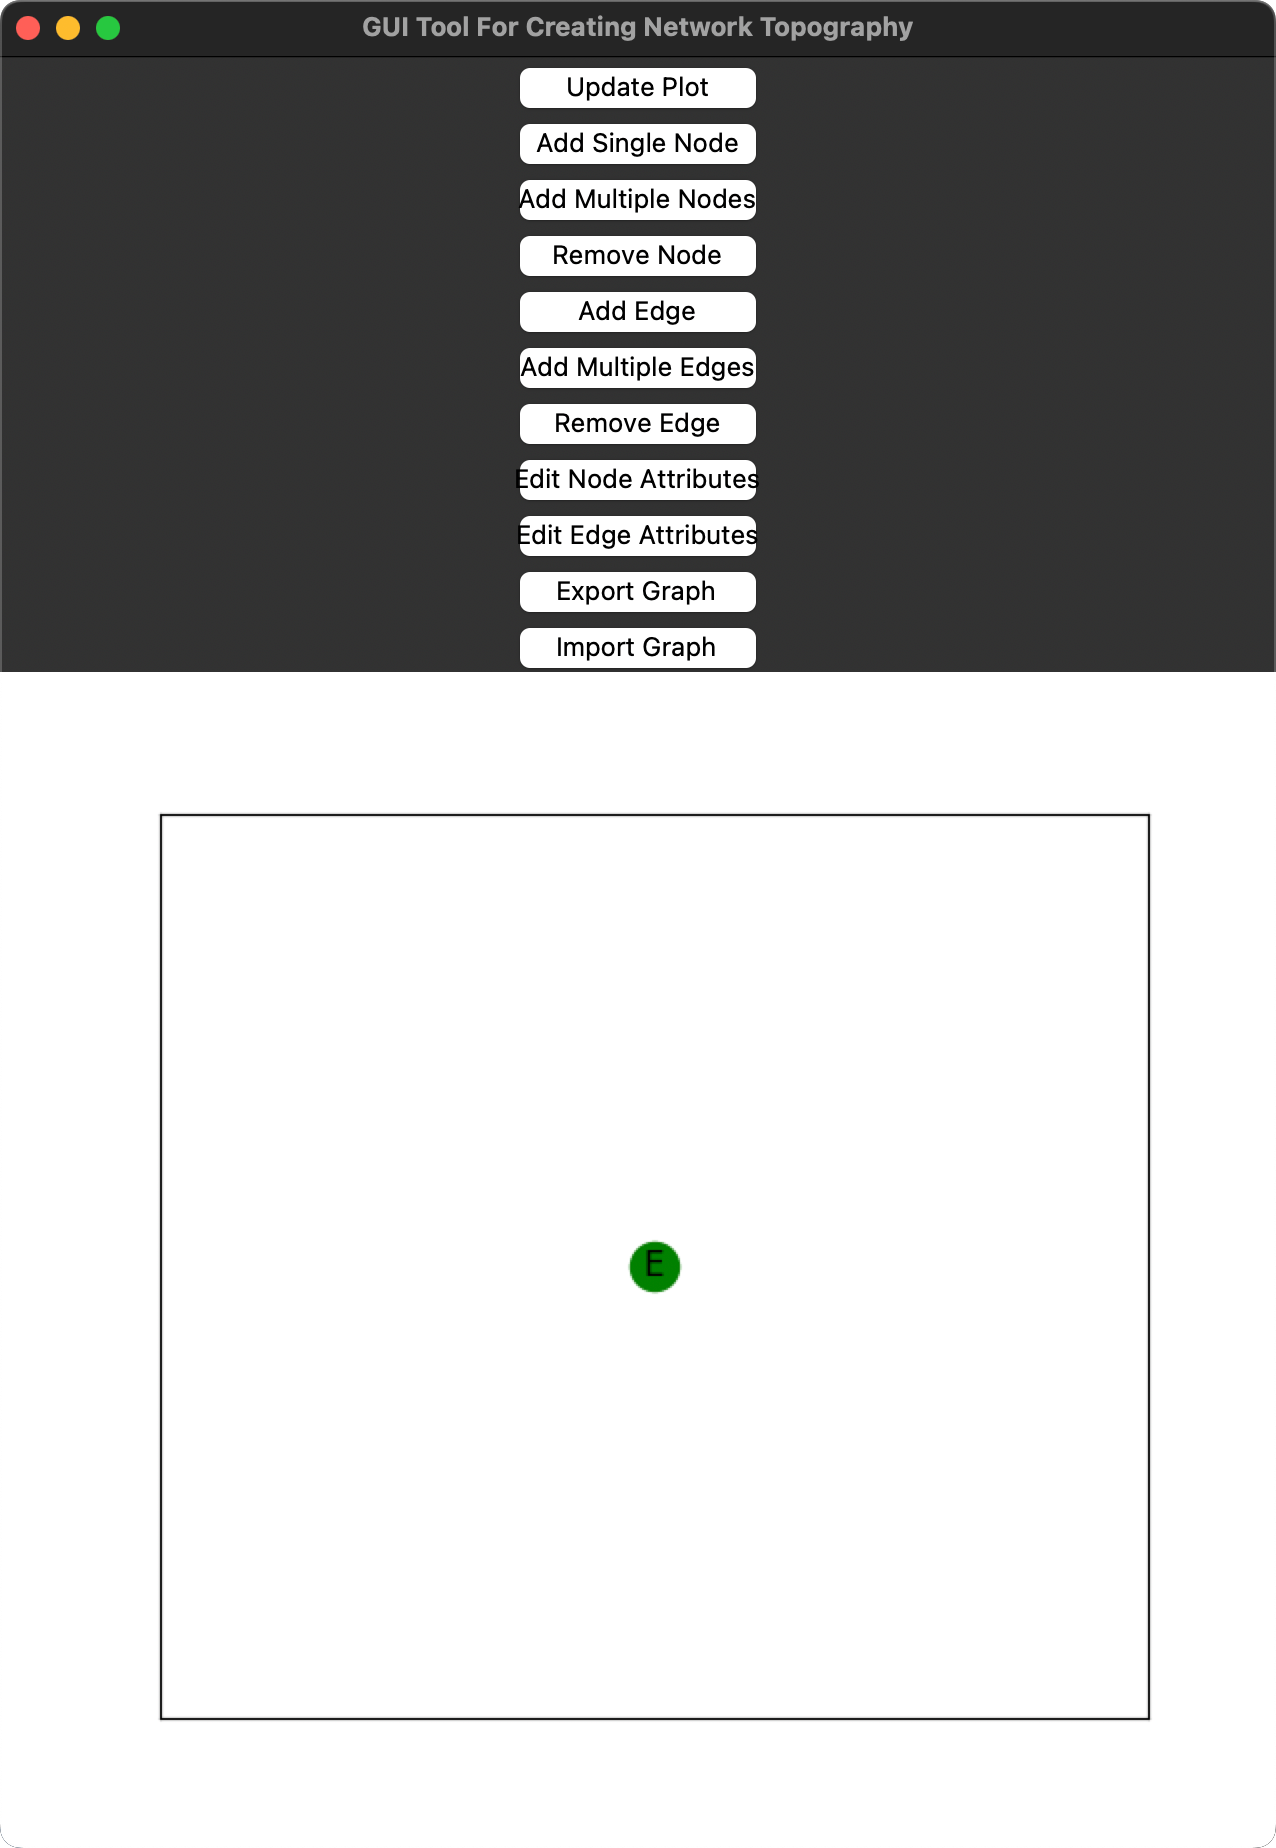
\includegraphics[width=\linewidth]{Screenshots/initial_startup_GUI_tool.png}
        \caption{
            The GUI tool as seen on the startup of the program.
        }
        \label{fig:ss:initial_startup_GUI_tool}
    \end{subfigure}
    \begin{subfigure}{0.49\linewidth}
        \centering
        \captionsetup{width=1\linewidth}
        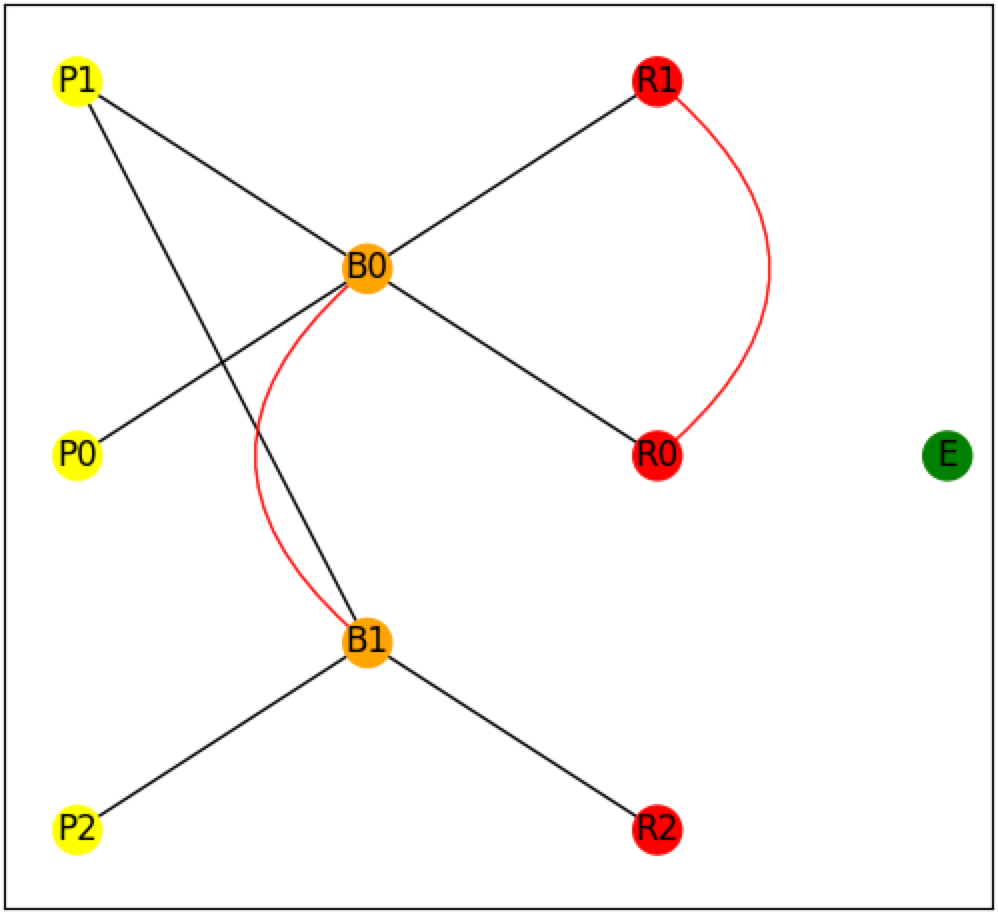
\includegraphics[width=\linewidth]{Screenshots/example_network.png}
        \caption{
            An arbitrary $3\times2\times3$ and $1\times 1 \times 1$ network with each node representing a phage, bacteria, or resource, with arbitrary interactions occurring between them. 
            Although not used here, edges between the same agent types and self loops are allowed. 
            This network topography along with a $1 \times 1 \times 1$ network will be used in the \nameref{Methods} and \nameref{AER} sections. 
        }
        \label{fig:ss:example_network}
    \end{subfigure} 
 \end{figure}

\subsection{Simulation Framework}
\label{sec:simulation_framework}
The user provides an ODE model and the network topography as input to the framework. 
The simulation framework deals with handling the input, output, collecting and storing of the simulation input and output.
The framework uses SciPy's \cite{virtanenSciPy10Fundamental2020} \textit{solve\_ivp()} numerical solver \cite{ dormandFamilyEmbeddedRungeKutta1980} to simulate the provided ODE equations and calculate the population levels through time.
The user receives two outputs from the framework. 
The first output is an array of time values that the solver used to calculate the population count.
The second output is an array containing the population count at each time step for every agent.

In order to facilitate more complex model behavior, "hidden" agents can be added to the simulation, where the hidden agents represent states that a "visible" agent can be in. 
Such an example would be the distinction between uninfected and infected bacteria. 
Each bacteria agent $b_i$ would contain two hidden sub-agents, called sub-agent states, an uninfected sub-agent state $b_{i_\text{uninfected}}$ and infected sub-agent state $b_{i_\text{infected}}$. 
It is possible to create further sub-agents, by having a bacteria go through $M$ stages of infection. 
So each infected agent has sub-agent $b_{i_{\text{infected}_k}}$, where $1 \leq k \leq M$. 

In the network model you would explicitly create a $3\times 2 \times 3$ network, but when passing the network to the simulation framework, you would tell the framework to model the subagents. 
The user's ODE model has to correctly model each (hidden) agent and correctly handle the changes in states. 

Even though the user might submit a $3 \times 2 \times 3$ model, if the user follows the uninfected and infected classification, where each bacterium goes through $4$ stages, the ODE model and framework will explicitly be modelling 3 phages, 10 bacteria (2 uninfected + $2\cdot 4=10$ infected bacteria), and 3 resources. 

The user might also be interested in modelling a resource reservoir in a chemostat, where resources go from an external reservoir not accessible by the bacteria to the virtual chemostat ready to be consumed by the bacteria. 
3 hidden resource agents would be added to the system, where the resources would model the transfer of resources from the reservoir to the simulation environment. 
The provided ODE model will have to correctly model and transfer the resources from $R_{i_{\text{reservoir}}}$ to $R_{j_{\text{chemostat}}}$. 

\subsection{Visualization Dashboard}
\label{sec:visualization_framework}
The third part involves analyzing and visualizing the simulation results on an interactive Dash Plotly \cite{DashDocumentationUser} dashboard. 
The user can use a dashboard built using Plotly Dash to interact with the solver and network.
The user can interact with the solver and network by changing parameter, environment, and setting values on the fly.
This allows the user to quickly change parameter values and test different situations.
The dashboard includes various starter plots that allow the user to test the model.
As output, the dashboard will show interactive plots so that the user can analyze the system. 


The dashboard allows the user to interact with the network, the model, and some prebuilt visualizations, and is built into three logical sections.
The first section allows for the user to edit the network parameters and setting values on the fly to quickly iterate through different conditions and to fine-tune parameter selection without having to rebuild the network using the GUI tool.
The second section allows for the user to see how the population count evolves over time for a given initial condition and parameter values, allowing to quickly test the network input.
The final section allows for the user to run more advanced analyses on the network, for example, by changing multiple parameter values and visualizing the output. 

\subsubsection{Editing Network and Parameter Values}
\label{sec:editing_network_and_parameter_values}
The editing network and parameter value contain five separate sections.
\paragraph{Initial Condition}
The initial condition settings panel (\Cref{fig:ss:ds:initial_condition}) allows for the user to edit the initial starting values of the agents. 
Each agent type has a table containing the initial population count. 
Extra hidden agents can be included. 
When a bacteria has been infected, the bacteria goes through multiple stages before lysing. Each bacteria agent starts out as uninfected, and once infected, the bacteria goes through 4 stages of infection before lysing as seen in \Cref{fig:ss:ds:initial_condition}.  
\paragraph{Vector Data} 
Data that can be represented as a vector, for example the data attributed to an agent type have their own section, \Cref{fig:ss:ds:vector}.
\paragraph{Matrix Data}
Data that is stored as a matrix, the data stored on edges between agents, is stored in the matrix tab (\Cref{fig:ss:ds:matrix}).
\paragraph{Environment and settings}
The environment data and settings data also have their own tab, \Cref{fig:ss:ds:environment} and \Cref{fig:ss:ds:settings} respectively.

\begin{figure}[!ht]
    \centering
    \begin{subfigure}{0.49\linewidth}
        \centering
        \captionsetup{width=1\linewidth}
        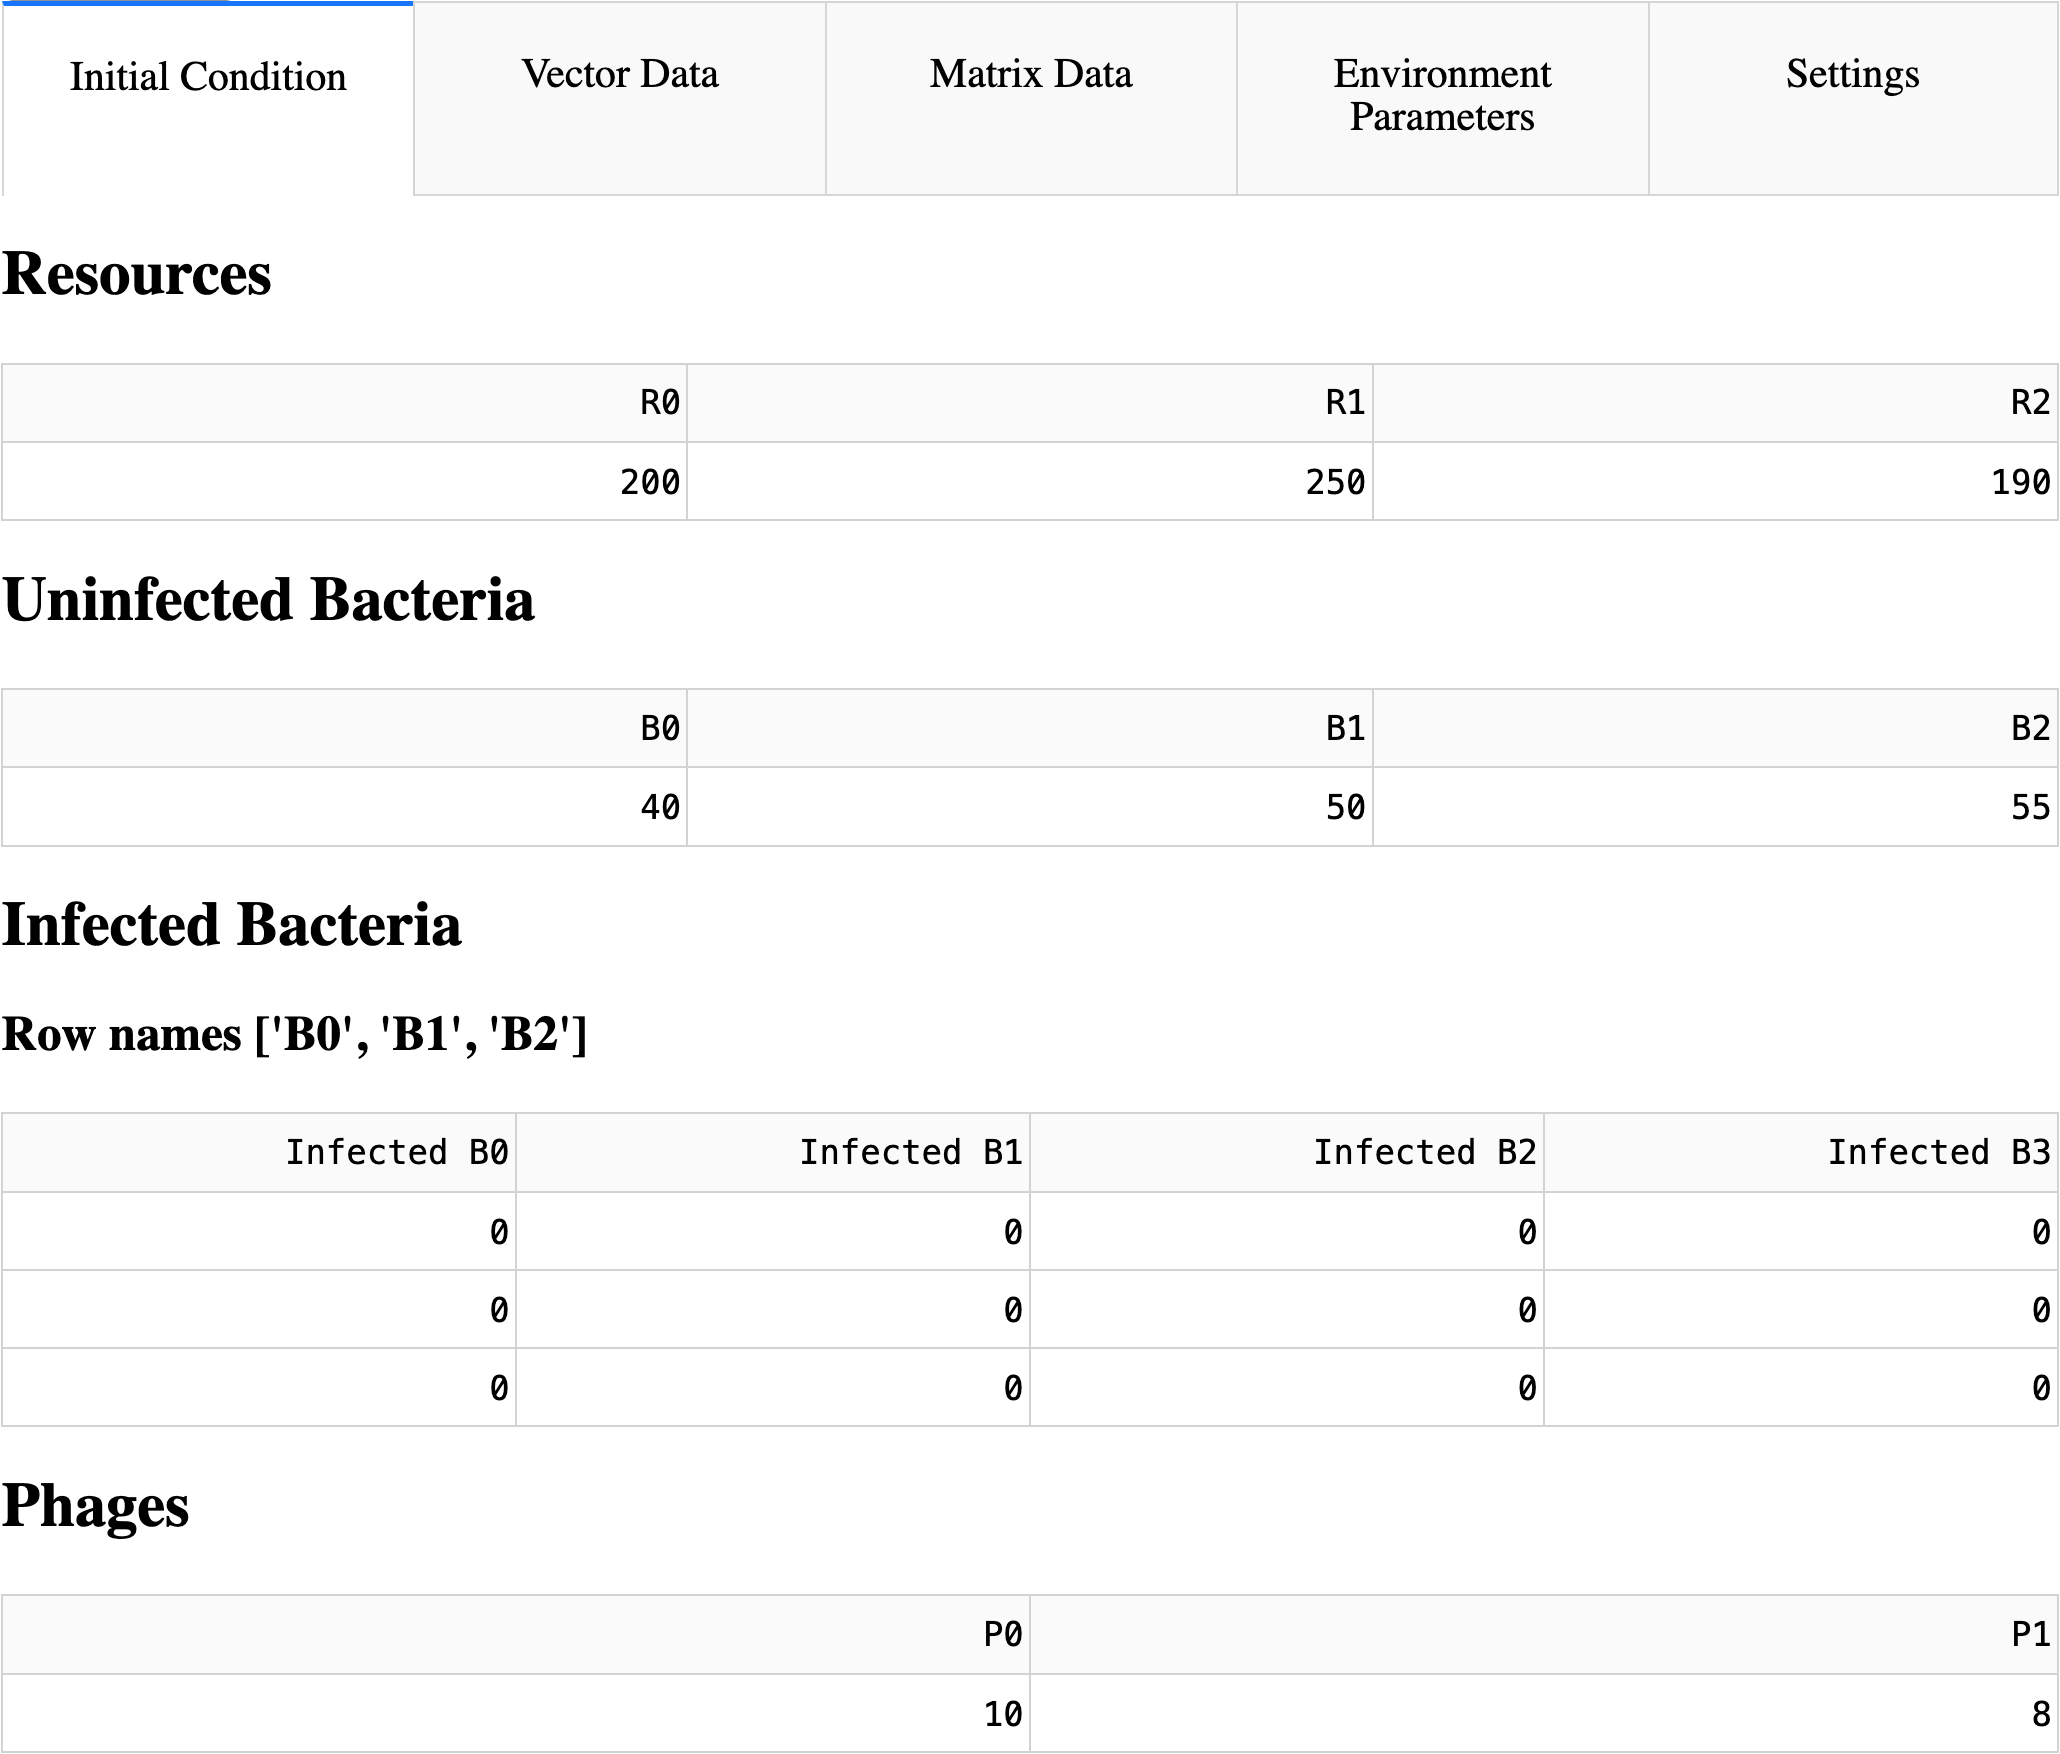
\includegraphics[width=\linewidth]{Screenshots/DashboardSettings/initial_condition_settings.png}
        \caption{
            The tab where the user can edit the initial conditions of the agents.
        }
        \label{fig:ss:ds:initial_condition}
    \end{subfigure}
    \hfill
    \begin{subfigure}{0.49\linewidth}
        \centering
        \captionsetup{width=1\linewidth}
        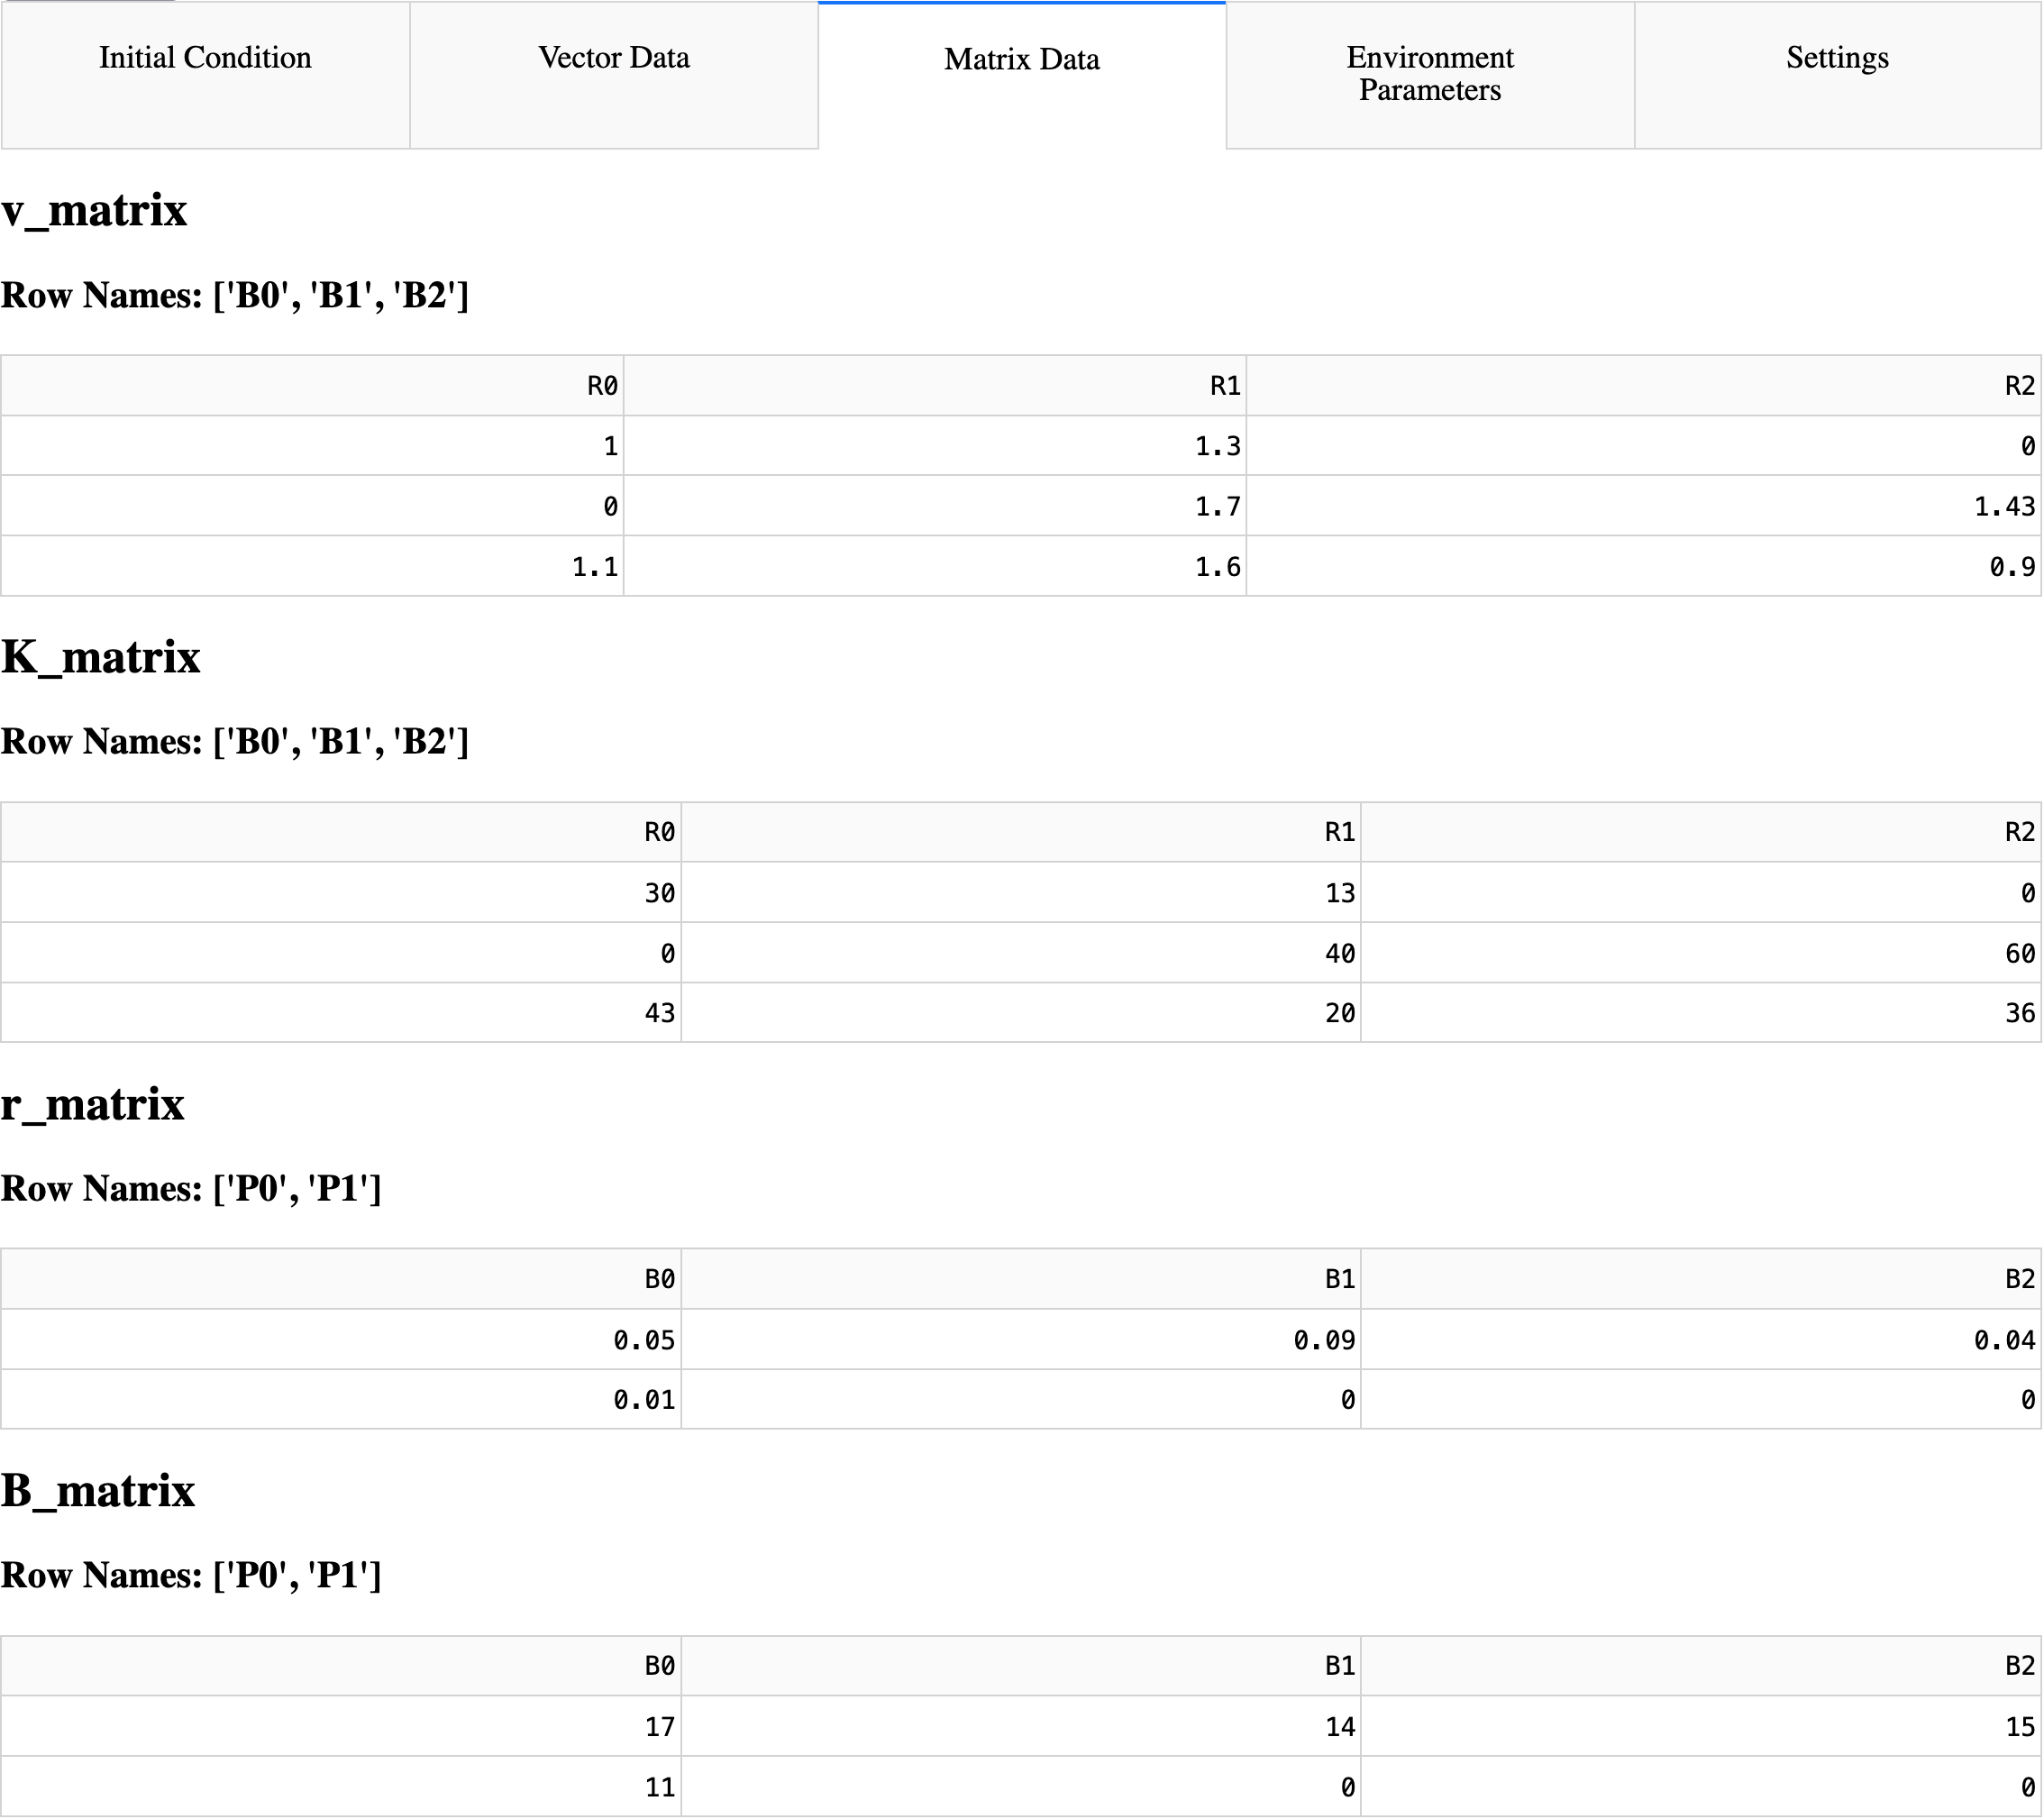
\includegraphics[width=\linewidth]{Screenshots/DashboardSettings/initial_matrix_settings.png}
        \caption{
            The tab where the user can edit the matrix attribute values. 
        }
        \label{fig:ss:ds:matrix}
    \end{subfigure}
    \hfill
    \begin{subfigure}{0.49\linewidth}
        \centering
        \captionsetup{width=1\linewidth}
        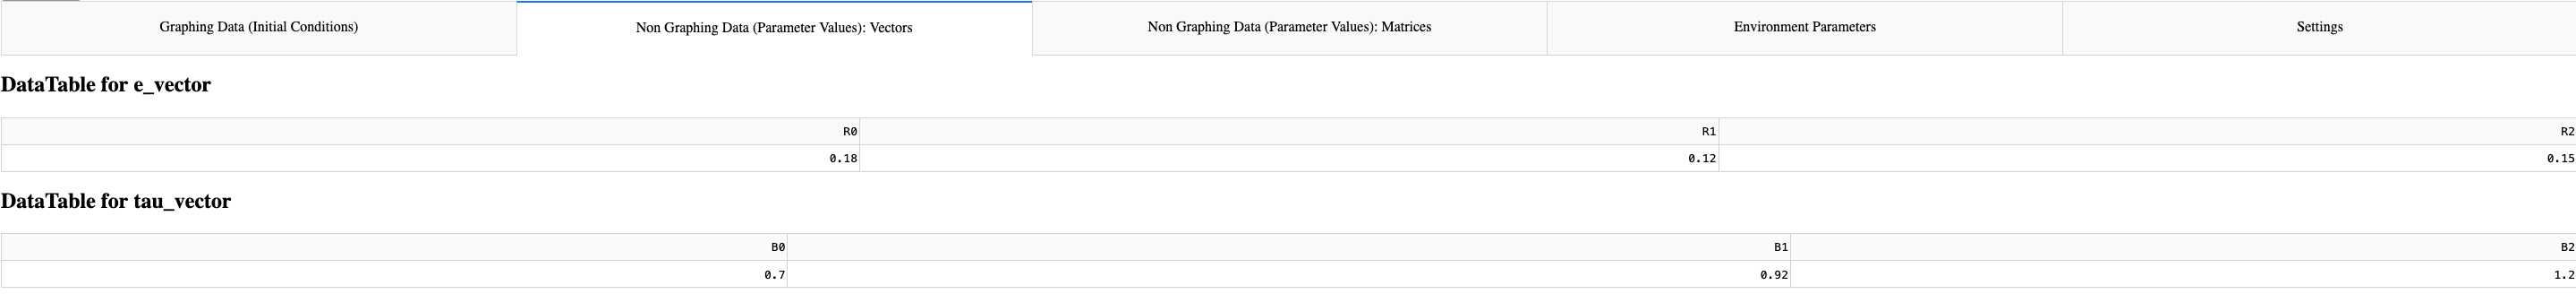
\includegraphics[width=\linewidth]{Screenshots/DashboardSettings/initial_vector_settings.png}
        \caption{
            The tab where the user can edit the vector attribute values.
        }
        \label{fig:ss:ds:vector}
    \end{subfigure}
    \hfill
    \begin{subfigure}{0.49\linewidth}
        \centering
        \captionsetup{width=1\linewidth}
        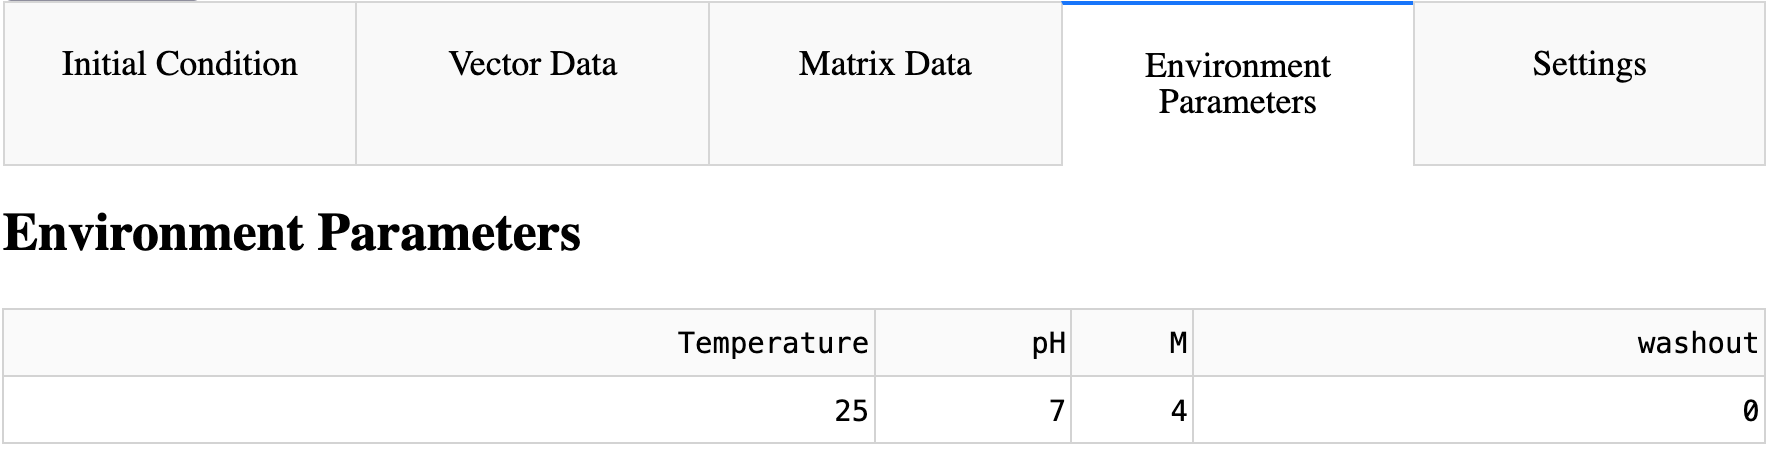
\includegraphics[width=\linewidth]{Screenshots/DashboardSettings/initial_environment_settings.png}
        \caption{
            The tab where the user can edit the environment values. 
        }
        \label{fig:ss:ds:environment}
    \end{subfigure}
    \hfill
    \begin{subfigure}{0.49\linewidth}
        \centering
        \captionsetup{width=1\linewidth}
        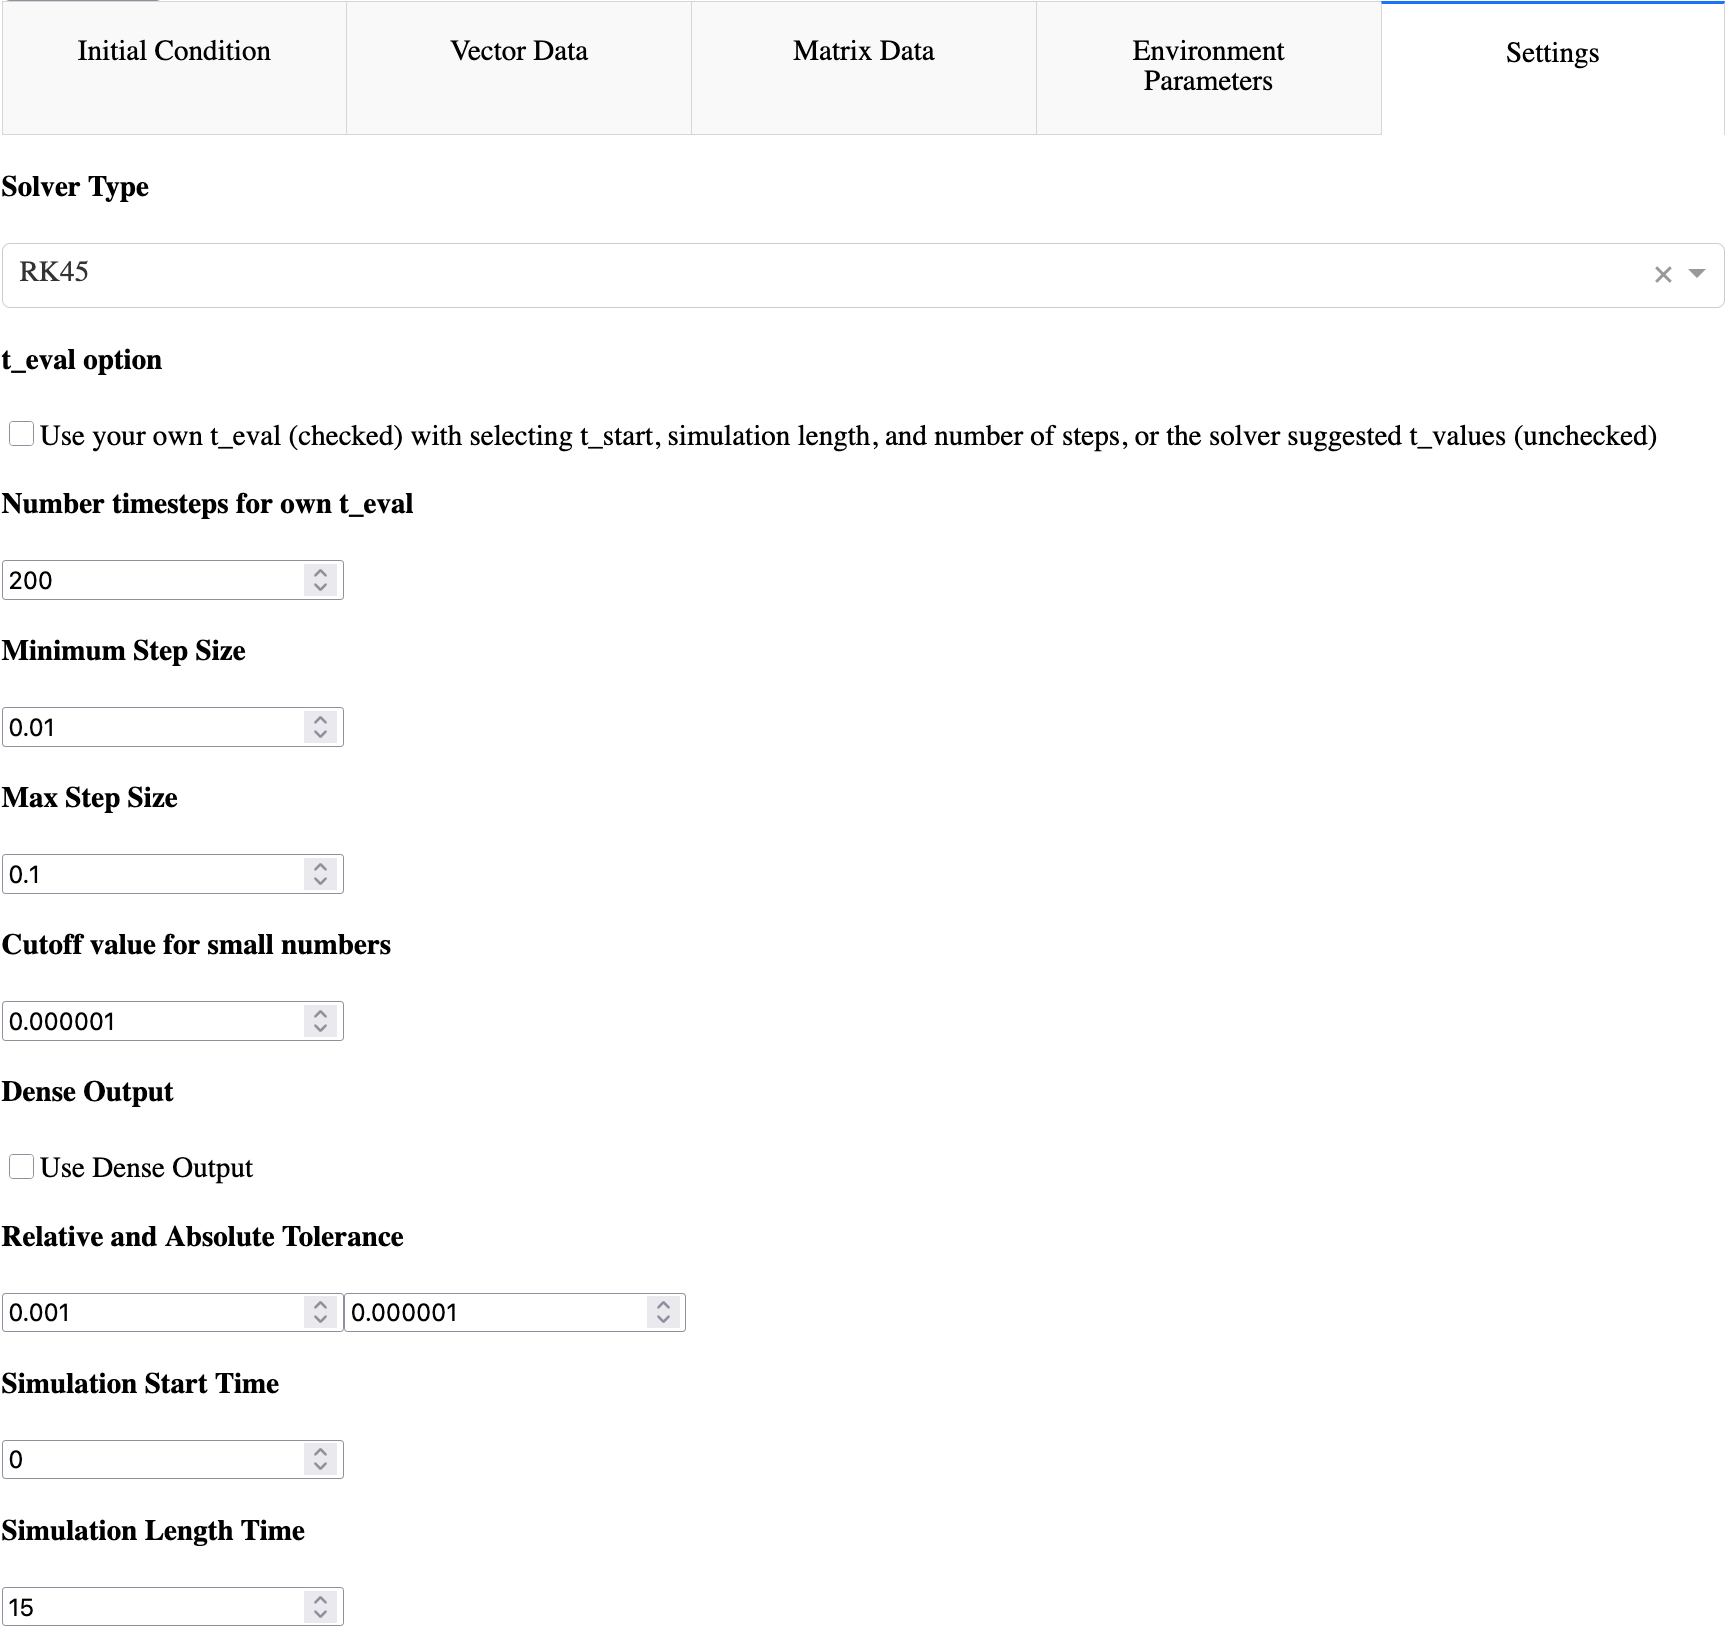
\includegraphics[width=\linewidth]{Screenshots/DashboardSettings/initial_settings_settings.png}
        \caption{
            The tab where a user can edit the settings of the solver and simulation. 
        }
        \label{fig:ss:ds:settings}
    \end{subfigure}
    \caption{The tabs where the user can edit the various parameter values and control the simulation parameters}
 \end{figure}

\subsubsection{Visualization and Analysis}
In the analysis section, the user can run different analysis methods to gain a greater understanding of the model.
For simplicity, the visualizations only support a $1 \times 1\times 1$ model, in order to make the analysis easier for the user, and to make it easier to analyze the visualization as the aim of the tool is to gain a deeper understanding of the interactions in a reduced complexity environment. 
These advanced visualizations were created with the mind of understanding a simple network.
There are five different analysis and visualization methods, and one system where the user can run a large simulation on the whole network and receive an output file containing the raw simulation file data.
The raw data is stored as a \textit{parquet} file, a tabular-like data format, which when combined with Dask \cite{DaskDaskDocumentation}, allows for querying of the data similarly to Pandas.
Parquet with Dask offers superior performance and data storage solutions that Pandas can't offer.
Once queried, the user can create their own graphs and plots as they have access to the parameter values used and the raw simulation data.

\paragraph{Serial Transfer}
\label{sec:serial_transfer}
Serial transfer is a method employed by bacteriologist where after a set amount of time, the bacteriologist pipettes a specified amount of media (for example 10ml of liquid) containing bacteria and resources, possibly with phages, and transfers the old media into a solution containing new media.
At this stage, the bacteriologist can introduce new agents, or re-introduce agents if the agent population or concentration has died out.
However, usually only resources are added during the transfer process.
An example would be an experiment starts with 50ml of solution.
The experiment runs for 24 hours before 5ml is removed.
Researchers can run various tests, such as using optical density measurements to assess bacterial density in the solution or employing a mass spectrometer to determine the concentration of the resources.
The 5ml is then re-added to a new solution of 45ml containing fresh resources.
The effect that this has is it creates a sort of artificial stable point.
As the bacteria grow, they consume the resources found in the solution.
However eventually the resources run out, and the bacteria die out due to a lack of resources.
By introducing new resources at set time intervals, the bacteria can regrow and exhibit a semi-stationary behavior.

The implementation of serial transfer is slightly different.
A user can select a number which will divide the population count of the agents by that number (\Cref{fig:ss:av:serial_transfer_settings}).
Then the program takes the initial condition values defined for the resources the initial condition in \Cref{sec:editing_network_and_parameter_values} and adds those values to the resources respectively.
By selecting a checkbox, the values as defined in the initial condition box for phages and bacteria in \Cref{sec:editing_network_and_parameter_values} can optionally be added as well.
As an example, if at the end of a simulation, there are 120 resources, 5000 bacteria, and 1000 phages remaining and the chosen serial transfer value is 15, then the resource, bacteria, and phage values would be decreased to 8, 333.33, and 66.66 respectively.
Then, if the initial condition for the resources, bacteria, and phages in \Cref{sec:editing_network_and_parameter_values} are 500, 80, and 10 respectively, and the checkbox is unchecked, the new population count will be 508, 333.33 and 66.66 respectively.
If the checkbox is checked, the new population count will be 508, 413.33, and 76.66 respectively.
These new values would be used as the new starting initial condition for a new simulation, and the run results will be appended to the previous run.
As output, new graphs are created showing the runs appended to one another, with an example output shown in \Cref{fig:ss:av:serial_transfer_run}.

\begin{figure}[!ht]
    \centering
    \begin{subfigure}{0.49\linewidth}
        \centering
        \captionsetup{width=1\linewidth}
        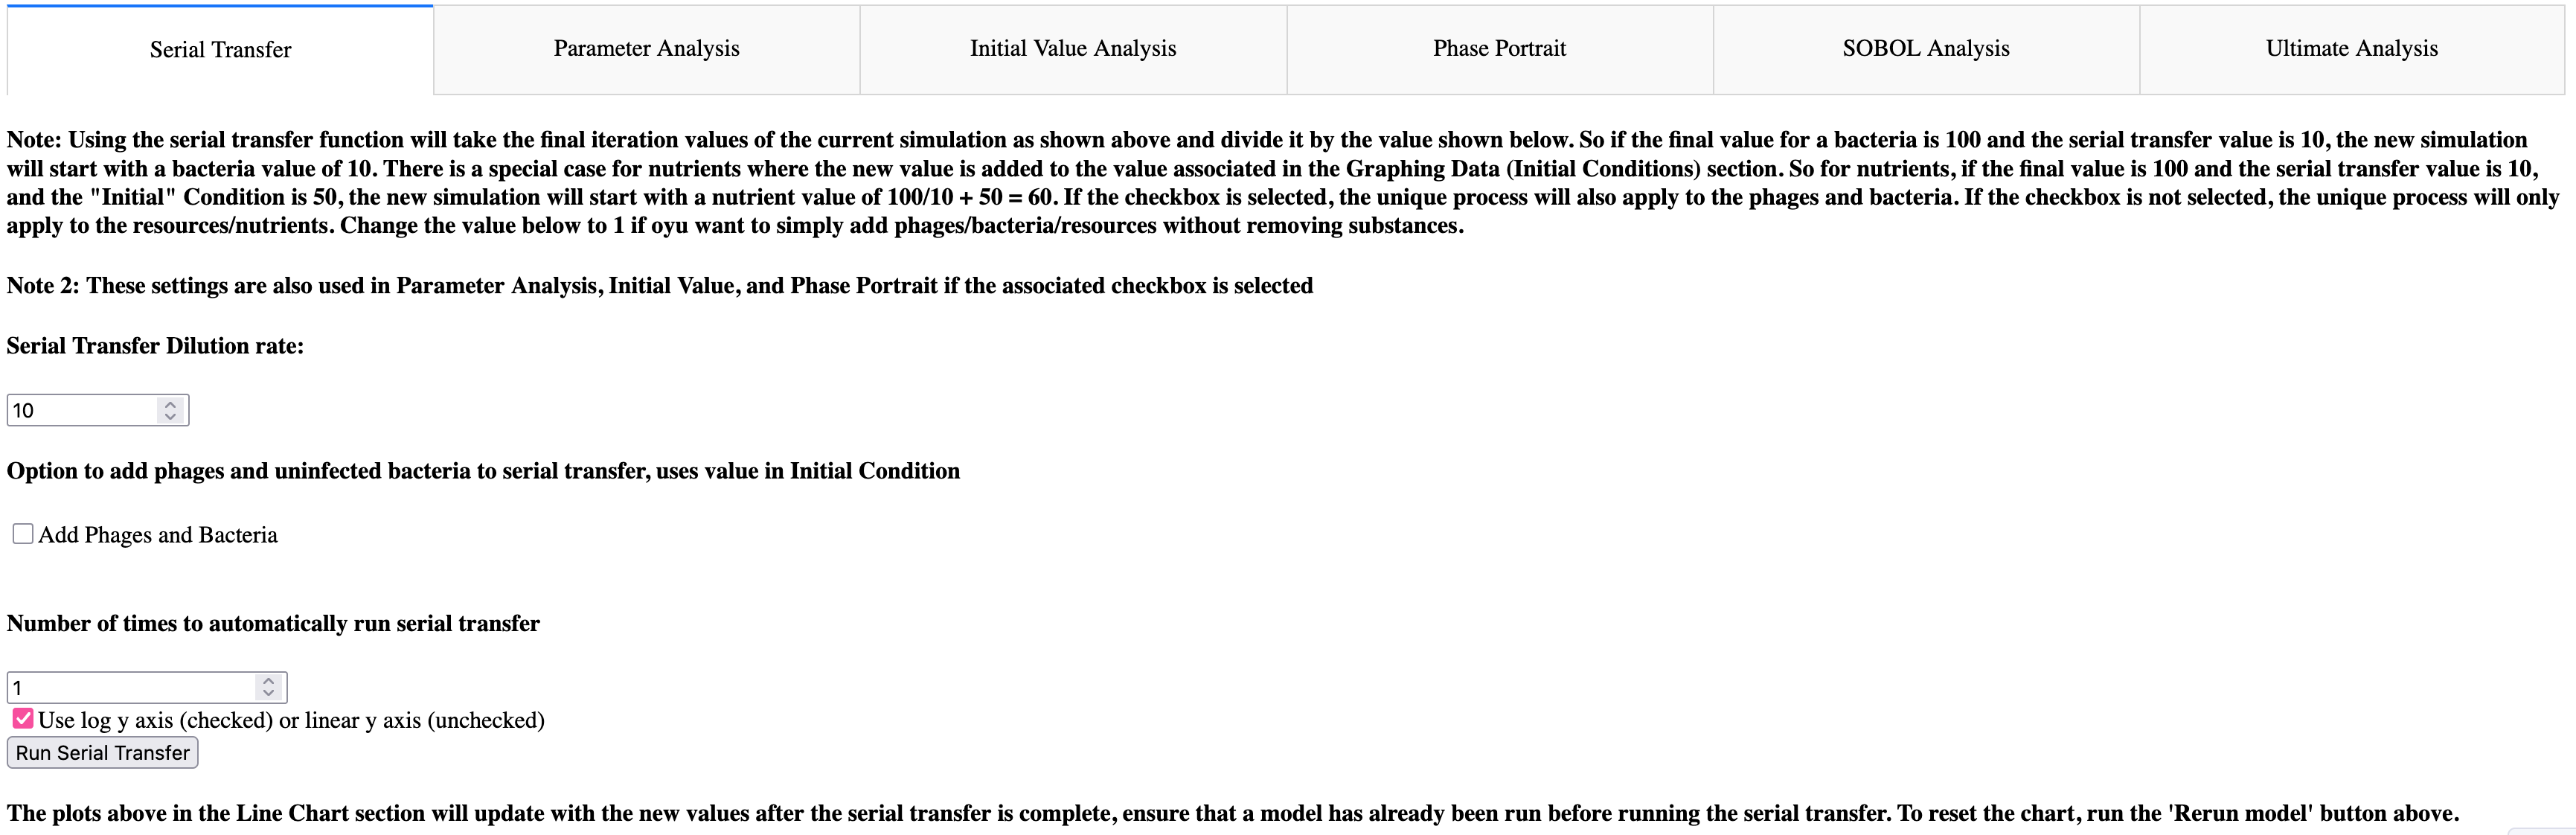
\includegraphics[width=\linewidth]{Screenshots/AdvancedVisualization/serial_transfer_settings.png}
        \caption{
            The section where the user can set up the serial transfer.
        }
        \label{fig:ss:av:serial_transfer_settings}
    \end{subfigure}
    \hfill
    \begin{subfigure}{0.49\linewidth}
        \centering
        \captionsetup{width=1\linewidth}
        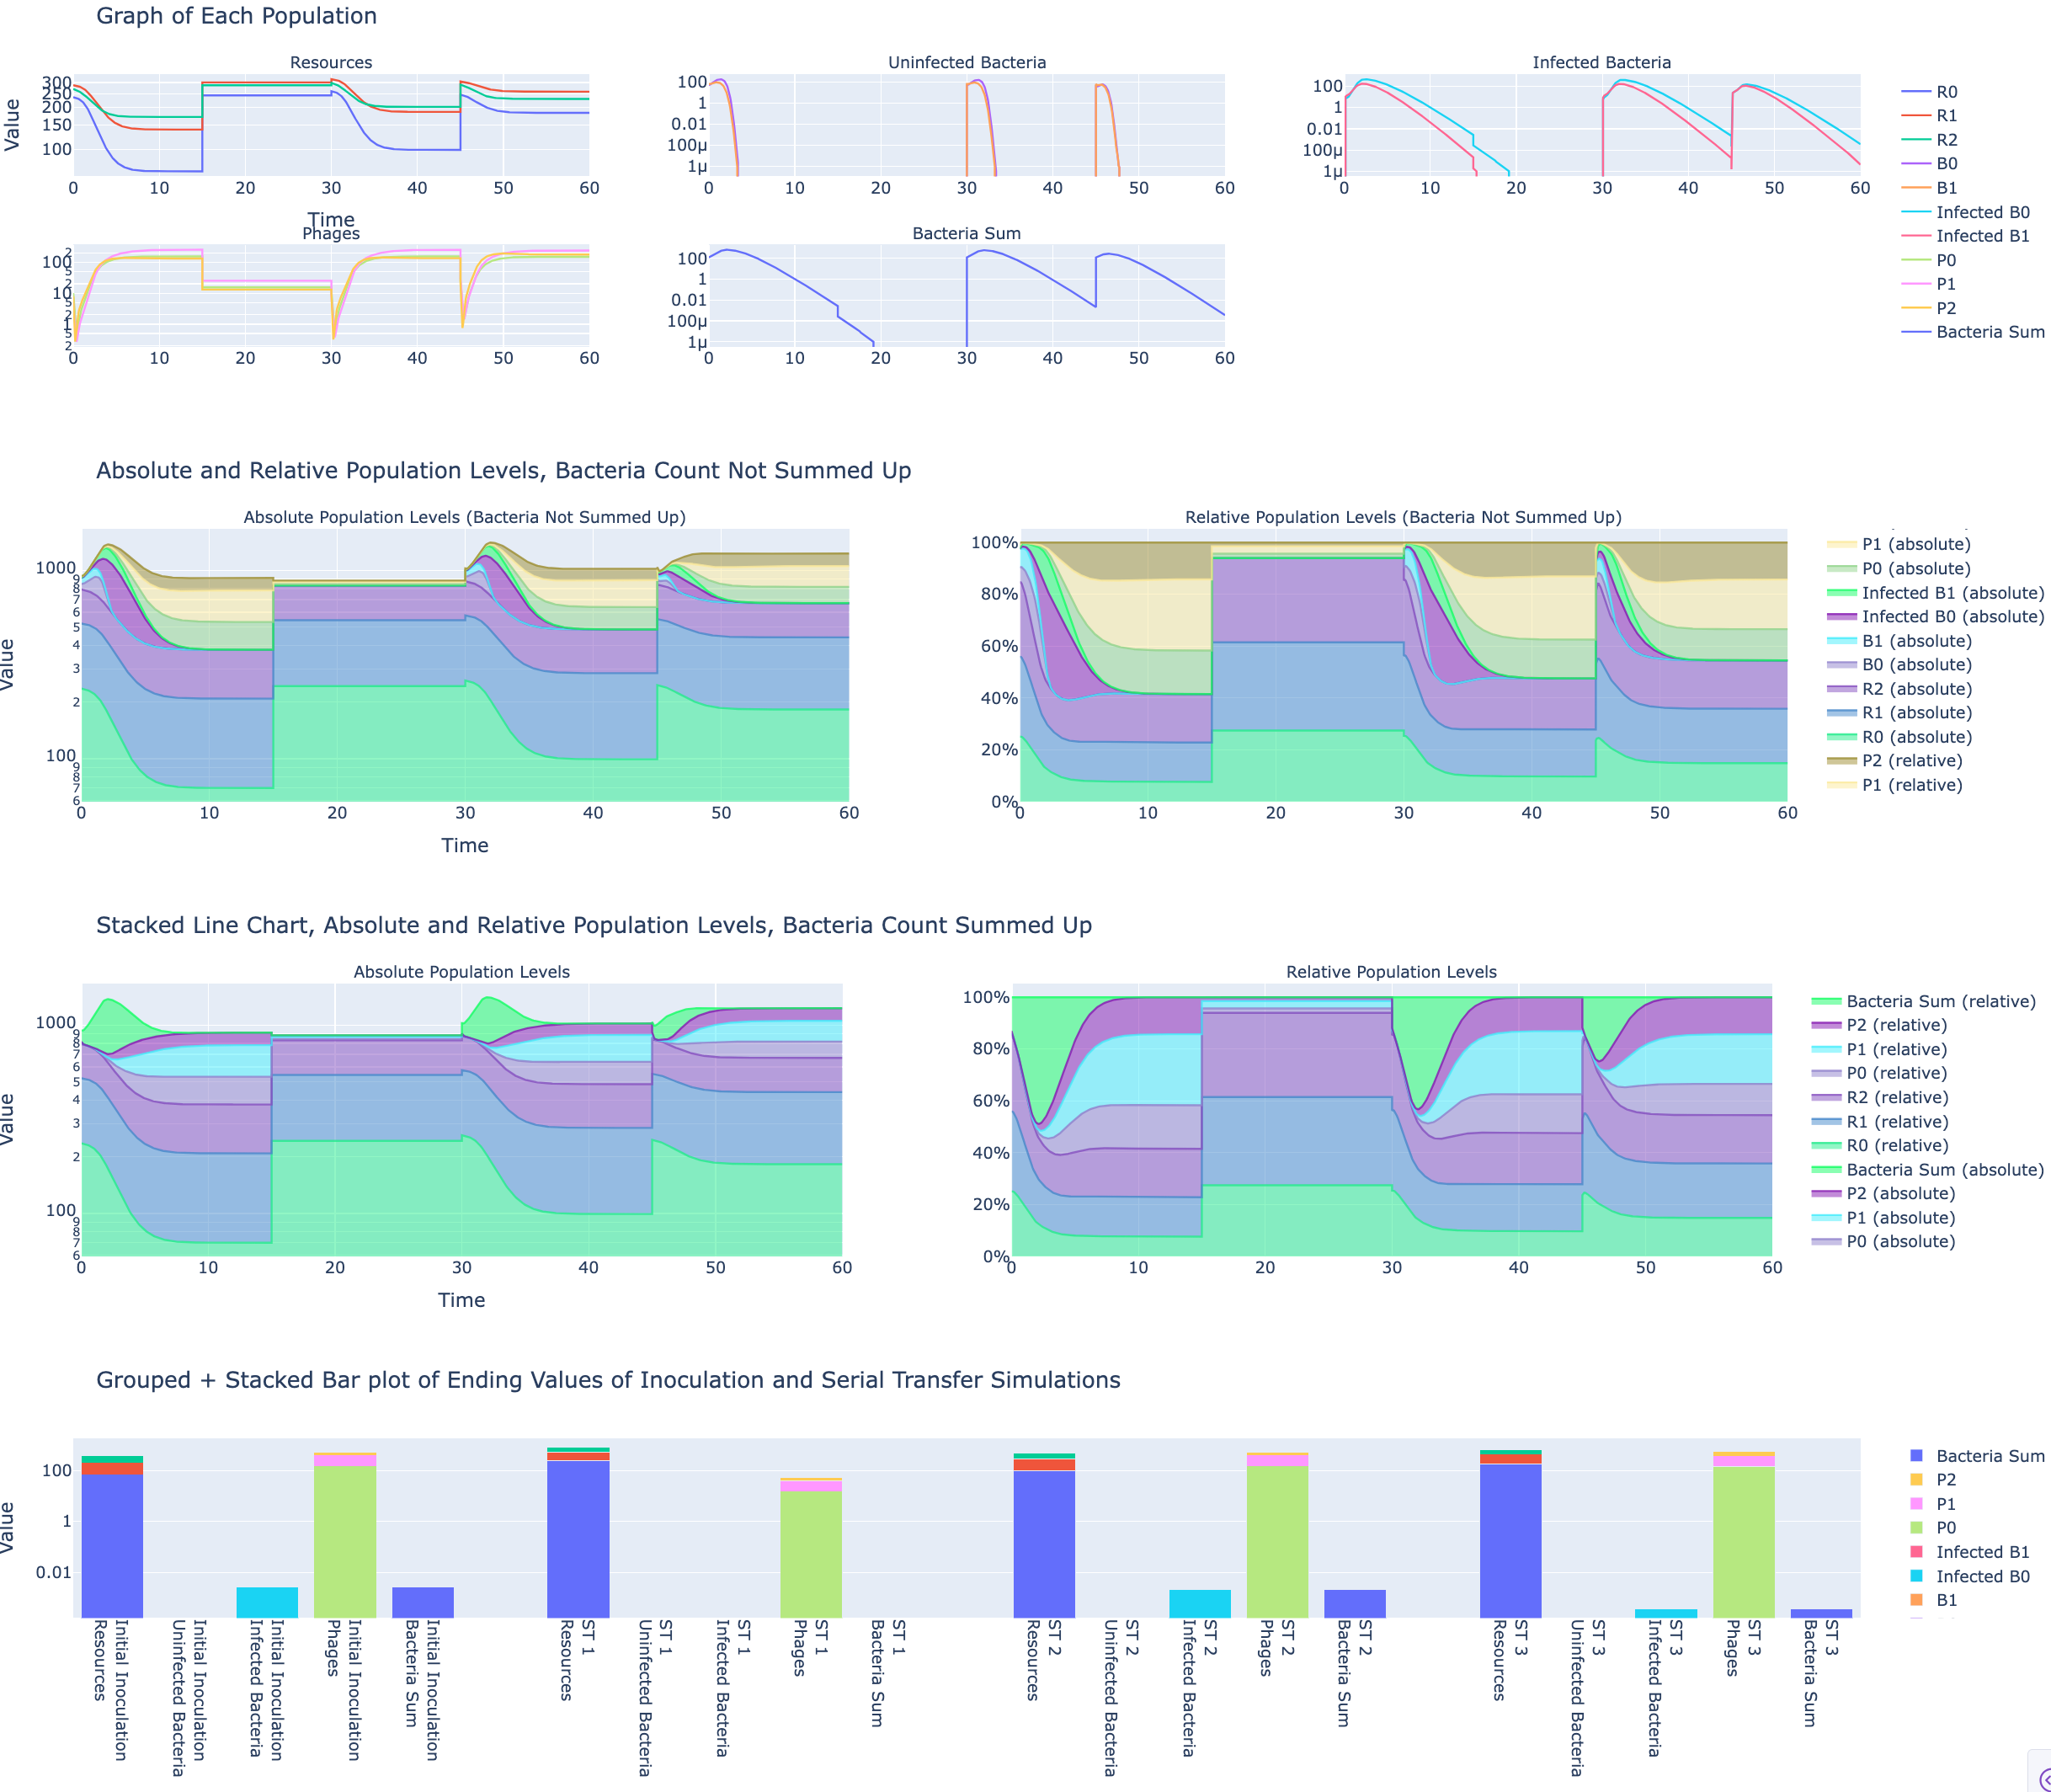
\includegraphics[width=\linewidth]{Screenshots/AdvancedVisualization/serial_transfer_run.png}
        \caption{
            The output plots of serial transfer. 
        }
        \label{fig:ss:av:serial_transfer_run}
    \end{subfigure}
    \caption{Serial Transfer}
 \end{figure}

\paragraph{Parameter Analysis}
\label{sec:parameter_analysis}
The parameter analysis settings tab as shown in \Cref{fig:ss:av:parameter_analysis_settings} allows the user to choose two parameters and individually run the model with the varying input values.
The values that can be tested and changed include all initial condition values, vector and matrix data, and environmental data.
As input, the user can select 2 parameters of choice.
After the parameter name selection, the user can manually choose which parameter values they want to test or test a range of values equally spaced by selecting the number of values to test.
Finally, the user can optionally run a serial transfer, where the serial transfer uses the settings found on the Serial Transfer tab. 

\Cref{fig:ss:av:parameter_analysis_run} shows the heatmap that the user can expect, one heatmap for each agent type.
Each heatmap cell represents the input of 2 unique parameter values, and shows the population count for that parameter run at the time shown in the slider. 
As the user slides the slider, the value inside the cell updates to correspond with the selected time. 
Note that the heatmap color range resets for each heatmap, so similar colors across heatmaps and across time will not correspond to the same values.

\begin{figure}[!ht]
    \centering
    \begin{subfigure}{0.49\linewidth}
        \centering
        \captionsetup{width=1\linewidth}
        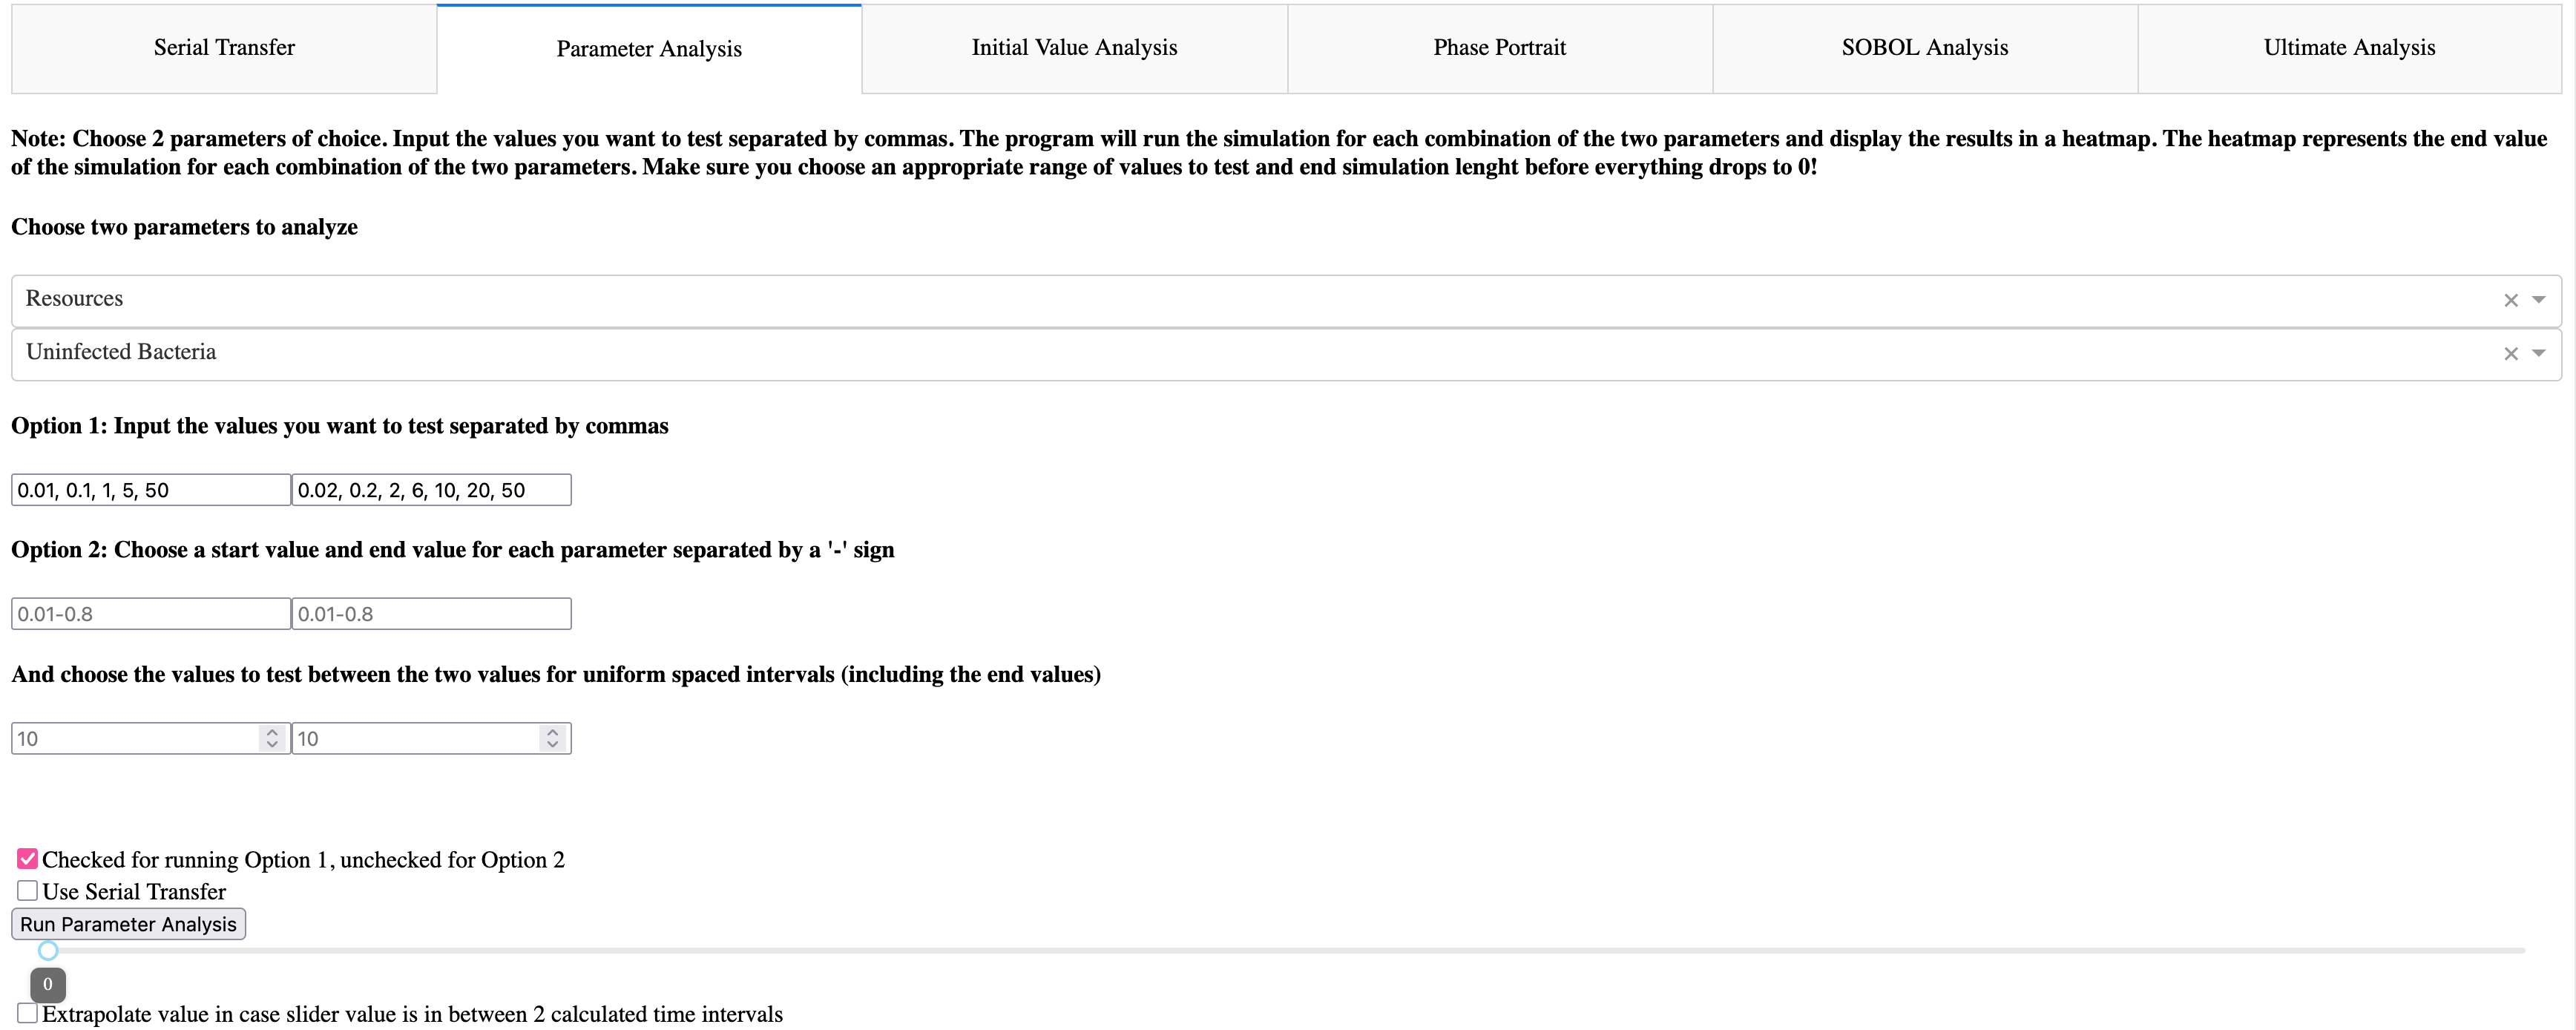
\includegraphics[width=\linewidth]{Screenshots/AdvancedVisualization/parameter_analysis_settings.png}
        \caption{
            The options available for the parameter analysis. 
        }
        \label{fig:ss:av:parameter_analysis_settings}
    \end{subfigure}
    \hfill
    \begin{subfigure}{0.49\linewidth}
        \centering
        \captionsetup{width=1\linewidth}
        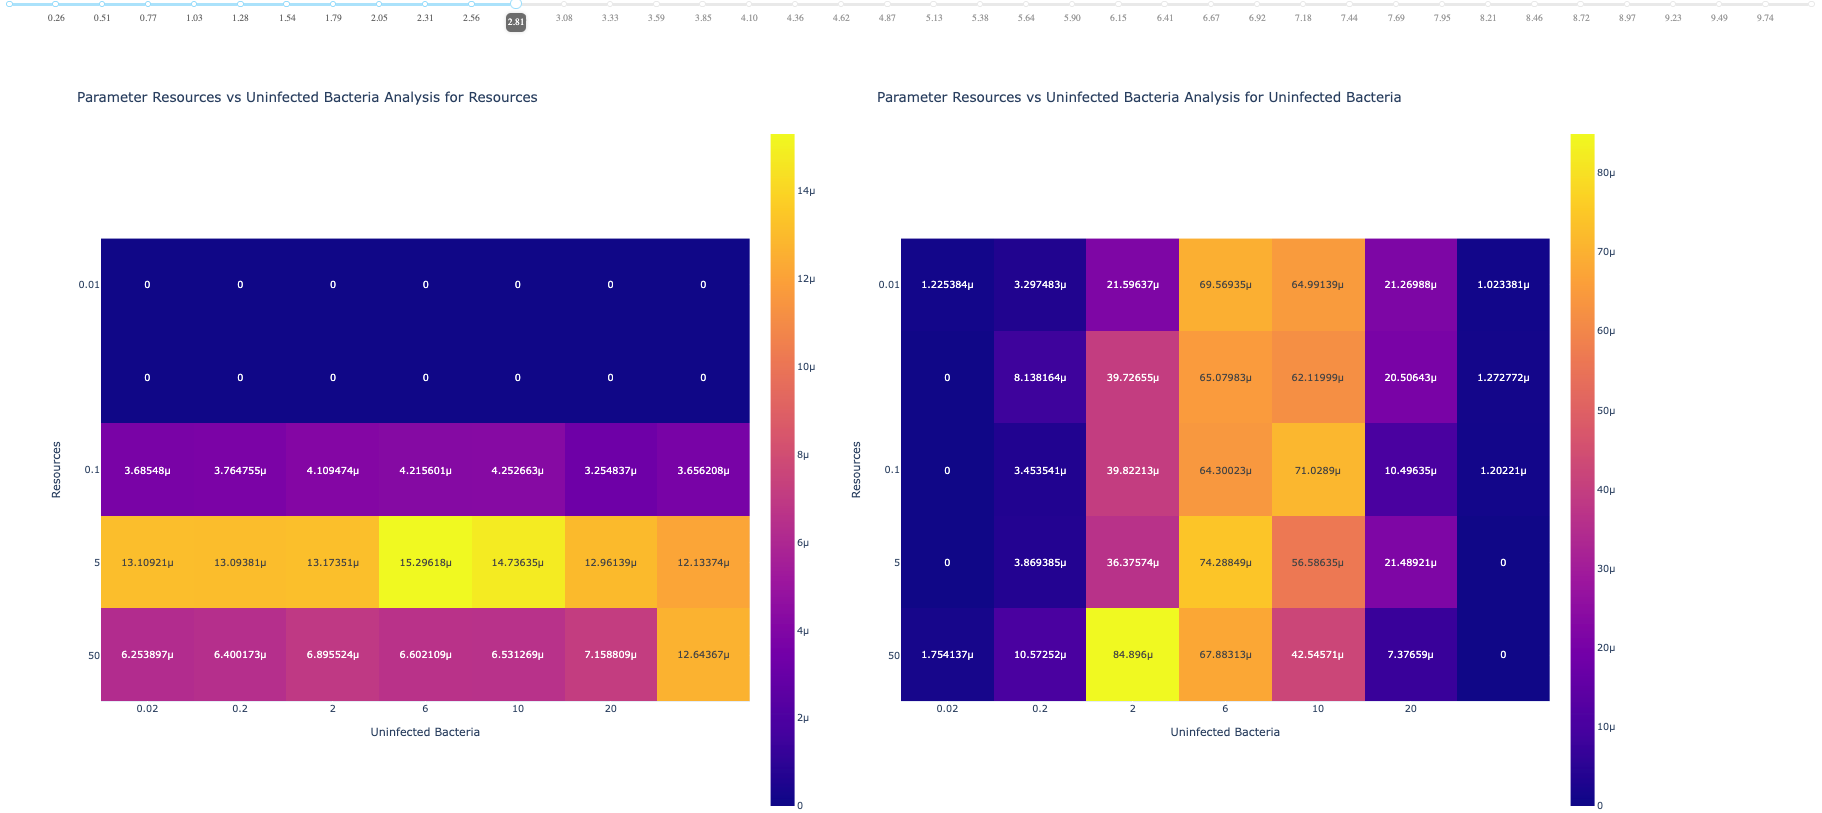
\includegraphics[width=\linewidth]{Screenshots/AdvancedVisualization/parameter_analysis_run.png}
        \caption{
            The output that the user can expect
        }
        \label{fig:ss:av:parameter_analysis_run}
    \end{subfigure}
    \caption{Parameter Analysis}
\end{figure}


\paragraph{Initial Value Analysis}
\label{sec:initial_value_analysis}
The initial value analysis settings tab as shown in \Cref{fig:ss:av:initial_value_analysis_settings} allows the user to choose a single parameter and vary the value of that parameter, visualizing how a change in parameter value affects the population count of the agents.

\Cref{fig:ss:av:initial_value_analysis_run} shows the plots that the user receives.
For each agent type, there are three plots made.
The left plot shows the population count through time, one line for each parameter value submitted.
The middle plot takes each run and calculates the “percentage from the max value“ (default value of $0.95 \rightarrow 95\%$) reached of the peak.
This value is considered the time of peak, and is used to fix some issues that can arise where the population plateaus or only keeps on rising.
The initial value is plotted on the x-axis, with the time at which the max value is reached on the y-axis.
Using the plotted data, a linear or log fit can be created.

The $R^2$ value, or coefficient of determination, is calculated as $R^2 = 1 - \frac{\sum_{i=1}^n (y_i - \hat{y}_i)^2}{\sum_{i=1}^n (y_i - \bar{y})^2}$
where $y_i$ is the observed values, $\hat{y}_i$ is the predicted values, and $\bar{y}$ is the mean of the observed values.

Using this data can be useful for understanding how a change in parameter value affects the time at which the population count reaches a maximum.
The slope, intercept and $R^2$ value is stored and saved in the third plot, a bar chart, with an editable name.
For every re-run of the initial value analysis, the slope, intercept and $R^2$ value is stored in the bar chart, allowing comparison of the slope-intercept data across different parameters. 

\begin{figure}[!ht]
    \centering
    \begin{subfigure}{0.49\linewidth}
        \centering
        \captionsetup{width=1\linewidth}
        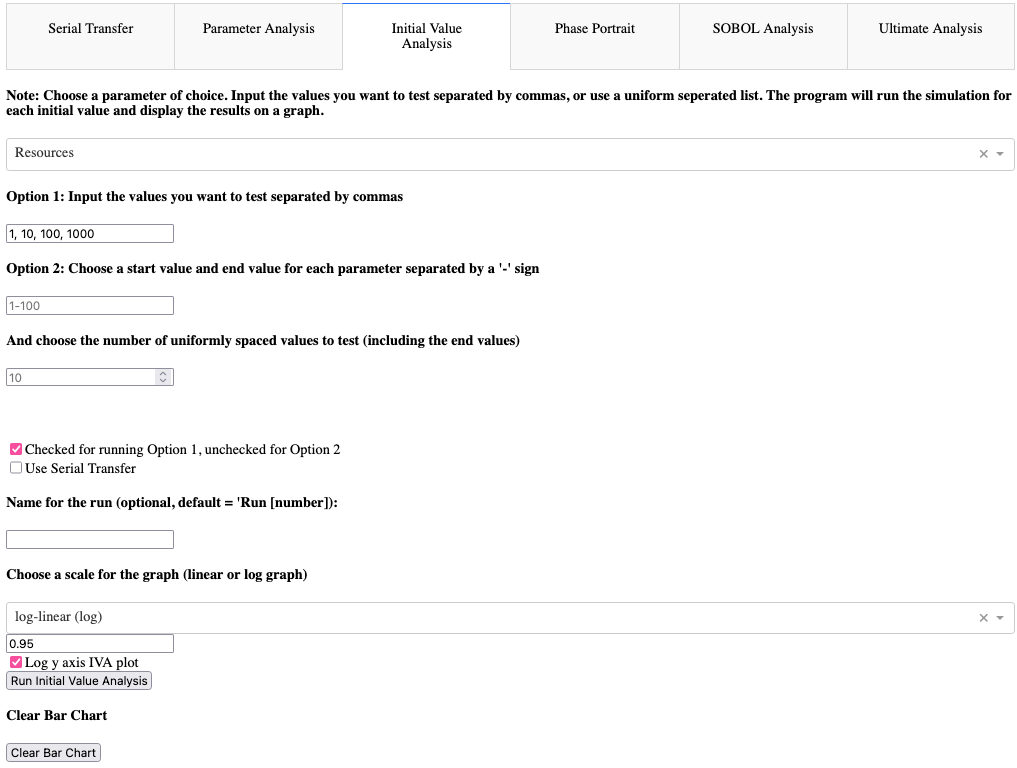
\includegraphics[width=\linewidth]{Screenshots/AdvancedVisualization/initial_value_analysis_settings.png}
        \caption{
            The settings for the initial value analysis tab. 
        }
        \label{fig:ss:av:initial_value_analysis_settings}
        \vspace*{\fill}
    \end{subfigure}
    \hfill
    \begin{subfigure}{0.49\linewidth}
        \centering
        \captionsetup{width=1\linewidth}
        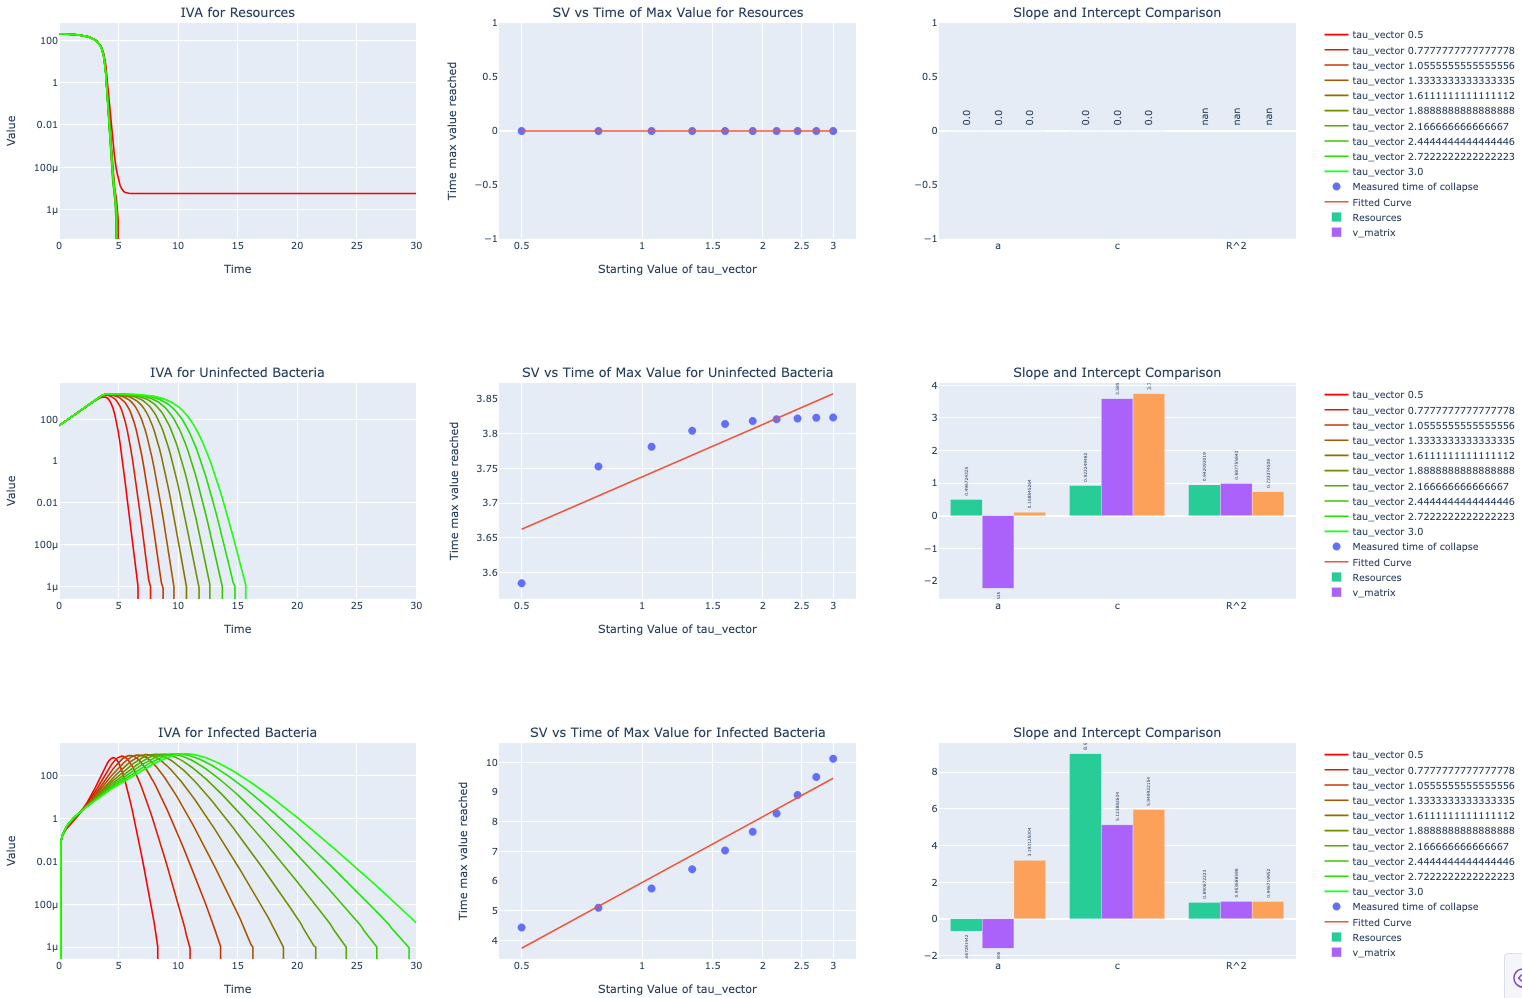
\includegraphics[width=\linewidth]{Screenshots/AdvancedVisualization/initial_value_analysis_run.png}
        \caption{
            An example initial value analysis output. 
        }
        \label{fig:ss:av:initial_value_analysis_run}
        \vspace*{\fill}
    \end{subfigure}
    \caption{Initial value analysis}
\end{figure}

\paragraph{Phase Portrait}
\label{sec:phase_portrait}
The phase portrait plot allows for the user to analyze how an agent population evolves with respect to the other agent population through time.
Phase portraits indicate how one population increases while the other decreases, and vice versa.
Steady states can be identified and classified as either stable, unstable, or as saddle points.
By comparing different starting points, it is possible to see if the system is chaotic or not.
The setup for the phase portrait can be seen in \Cref{fig:ss:av:phase_portrait_settings}, and a sample output can be seen in \Cref{fig:ss:av:phase_portrait_run}. 

\begin{figure}[!ht]
    \centering
    \begin{subfigure}{0.49\linewidth}
        \centering
        \captionsetup{width=1\linewidth}
        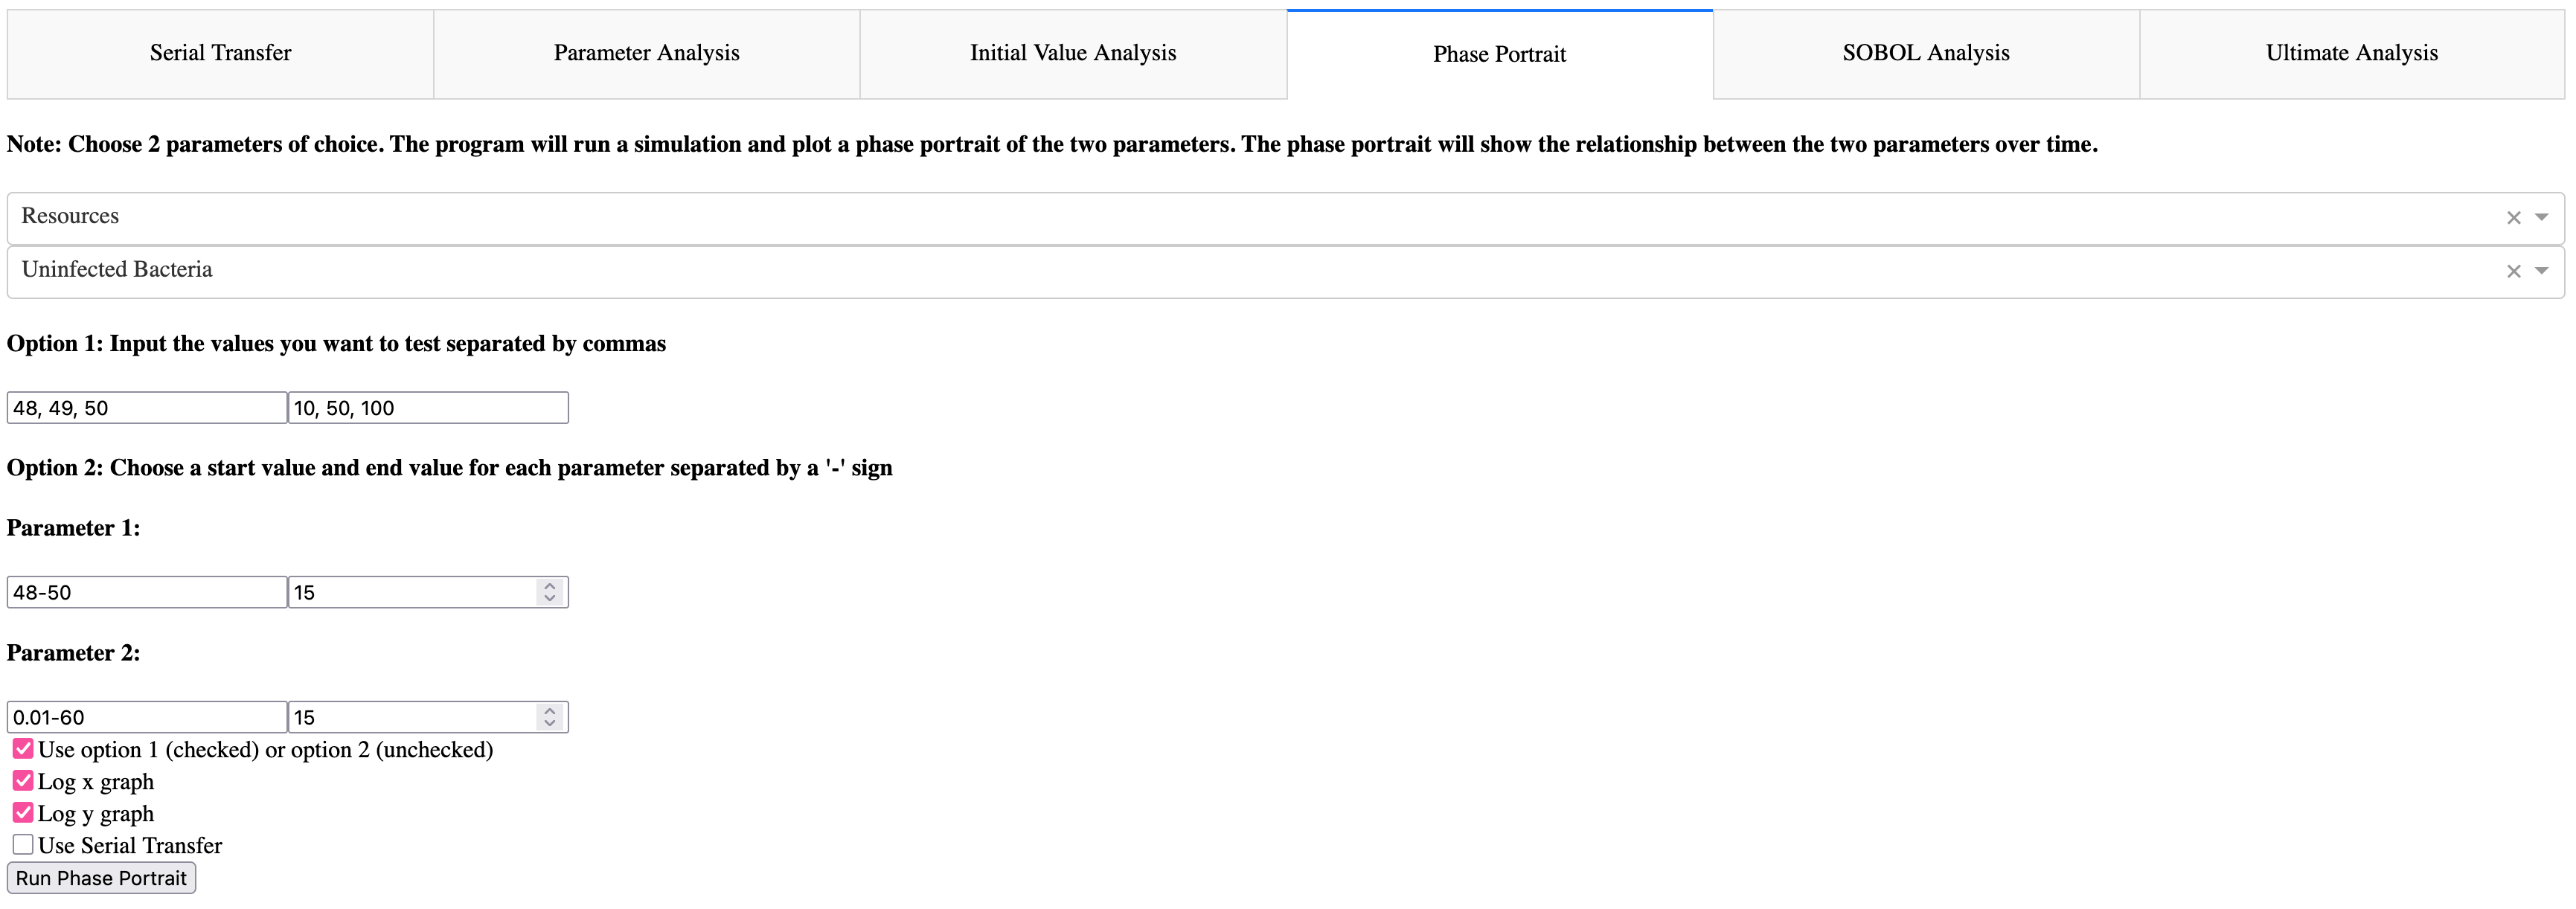
\includegraphics[width=\linewidth]{Screenshots/AdvancedVisualization/phase_portrait_settings.png}
        \caption{
            The user can select two starting values for the initial condition, but they can't choose vector, matrix, or environment settings due to the plot showing the development of agent populations against other agent populations.
            As typical, the user can select their own values or auto-generate values between two values, as well as use a serial transfer option.
            There is also an option to take the logarithm of the x and/or y-axis. 
        }
        \label{fig:ss:av:phase_portrait_settings}
    \end{subfigure}
    \hfill
    \begin{subfigure}{0.49\linewidth}
        \centering
        \captionsetup{width=1\linewidth}
        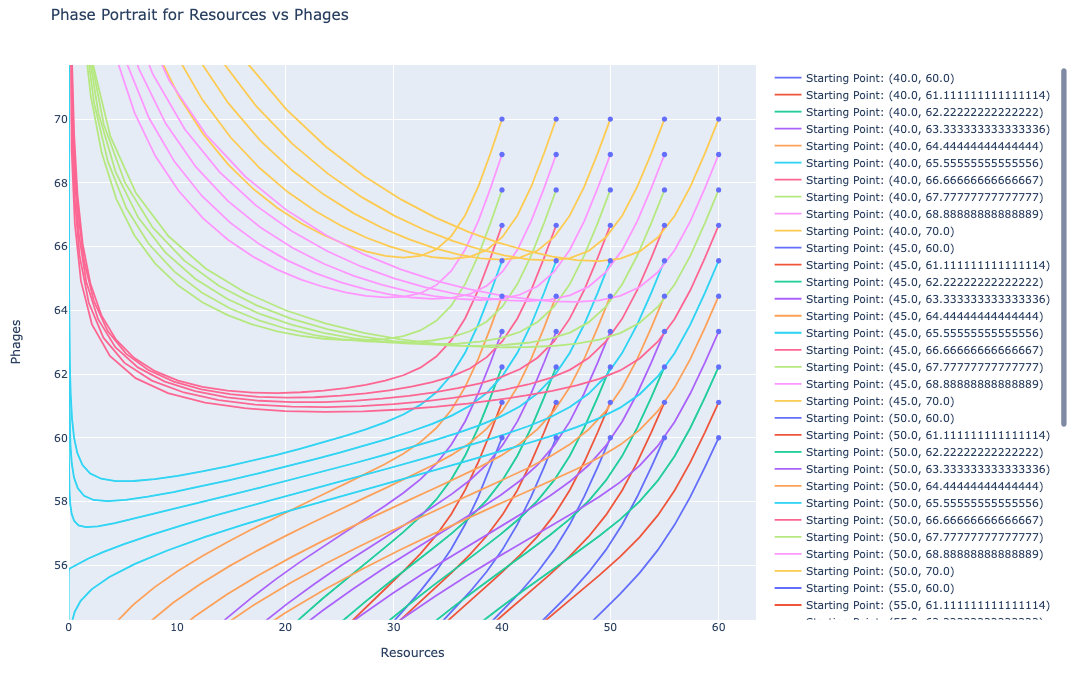
\includegraphics[width=\linewidth]{Screenshots/AdvancedVisualization/phase_portrait_run.png}
        \caption{
            An example run of a phase portrait.
        }
        \label{fig:ss:av:phase_portrait_run}
    \end{subfigure}
    \caption{Phase Portrait}
\end{figure}

\paragraph{SOBOL Sensitivity Analysis}
\label{sec:SOBOL_sensitivity_analysis}
SOBOL analysis, a variance-based sensitivity analysis, is a method that allows a user to quantify how important an input parameter has on a measured aspect of the output by changing the parameter values of the model and measuring the change in model output.
SOBOL quantifies how much variance in the output can be attributed to a specific parameter and can measure the effect of global/total ($ST$), first ($S1$), and second order sensitivity ($S2$). 
Global, also called total sensitivity, is the summation of all higher order interactions. 
First order $Si$, or local sensitivity, is the measurement of the effect that parameter $i$ has on the variance of the output. 
Second order is the measurement of parameter $i$ interacting with parameter $j$, nad how the interaction attributes to the output variance. 
Etc for third order and higher. 
When $ST_i >> S1_i$ then parameter $i$ depends on interactions with other parameters, while when $ST_i \equiv S1_i$, then $i$ doesn't interact much with and depend on other parameters.
It should be stated that $ST_i \geq S1_i$. 

When a model is viewed as a black-box model, the model can be seen as a function $Y=f(X)$, where $X$ is an input vector of $d$ elements, and $Y$ is a univariate model output.
$X$ is assumed to be independently and uniformly distributed within a hypercube $X_i \in [0, 1]$ for $i=1, \dots d$.
The first order sensitivity measures the output variance of the main affect of parameter $X_i$.
Measuring the effect of varying $X_i$ averaged over other input parameters, and standardized to provide a fractional contribution to the overall output variance.
The first order sensitivity is described as
\[
    S1_i = \frac{V_i}{\textit{Var}(Y)}
\] where $V_i = \textit{Var}_{X_i}(\mathbb{E}_{X_{\sim i}}[Y|X_i])$ and where $X_{\sim i}$ represents all the parameters that are not $X_i$.
All parameters are summarized in \Cref{tab:parameter_table_SOBOL}

The second order index measures the impact of input $X_i$ interacting with $X_j$. For many inputs, this becomes unwieldy to analyze.
The global sensitivity is used to analyze the global sensitivity without evaluating $2^d-1$ indices, and measures the contribution to the output variance of $X_i$, including all variance due to $X_i$'s interaction with other variables.
\[
    S1_i = \frac{\mathbb{E}_{X_{\sim i}}[\textit{Var}_{X_i}(Y|X_{\sim i}))}{\textit{Var}(Y)} = 1 - \frac{\textit{Var}_{X_i}(\mathbb{E}_{X_i}[Y|X_{\sim i}])}{\textit{Var}(Y)}
\]
SOBOL can analyze various univariate outputs.
This could be either the average value of an agent population, the variance in population count, the time at the peak of an agent count, the final population value, etc. \newline
SOBOL accepts a list of parameter names and a list of range of values to sample from, which the user can input in the SOBOL settings tab, \Cref{fig:ss:av:SOBOL_analysis_settings}. 
If no values are added, the parameter is not included in the simulation and the default value is instead used. 
The user then needs to select the number of samples to run, using the formula $2^x$, where $x$ is the number they input, and $2^x$ is the number of samples that SOBOL will create and run.
The larger $x$ is, the more accurate the SOBOL analysis results will be, but the more simulations would need to be run. \newline
Otherwise, if 2nd order is not chosen, the model is run $N(D+2)$ times.
If the user wants to analyze the second order interactions, then the model will run the system $N(2D+2)$ times with the randomly sampled input values, where $N$ is a multiple of 2, and $D$ is the number of parameters being tested.
Due to the randomness of the sampling method, the user can, but does not need to, submit a seed value. 

Three SOBOL analyses are included by default in the dashboard, as shown in \Cref{fig:ss:av:SOBOL_analysis_run}.
An analysis of the final value of the simulation, the average population count, and the variance in population count.
The global and first sensitivity are shown next to one another, and each sub-row within a plot represents each agent type. 
The proportion of the global and local sensitivity can be seen for each agent type and each parameter.

It can be argued that the final, average, and variance value of the run is not a useful statistic to measure and run a SOBOL analysis on. 
One might give the reasoning that the population value at time $t$ depends on the previous time step $t-1$. 
Thus the average and variance of the value is not completely random and is semi dependent on the previous value. 
Another argument is that the simple golden model doesn't exhibit complex behavior unlike the output exhibited in \Cref{fig:cocktail_plot}. 

Making a dashboard that can be used for different inputs is hard to make. Predicting the type of plots that a user might be interested in, and the type of behavior the user wants to analyze is impossible to predict. 
Therefore, three simple and easy to understand default SOBOL analysis methods are provided that aims to capture the simple dynamics of the system. 
Upon completion of a SOBOL analysis, the original simulation data is stored to the disk as a \textit{.pickle} file so that the user can use the data and run their own SOBOL analyses. 

\begin{figure}[!ht]
    \centering
    \begin{subfigure}{0.49\linewidth}
        \centering
        \captionsetup{width=1\linewidth}
        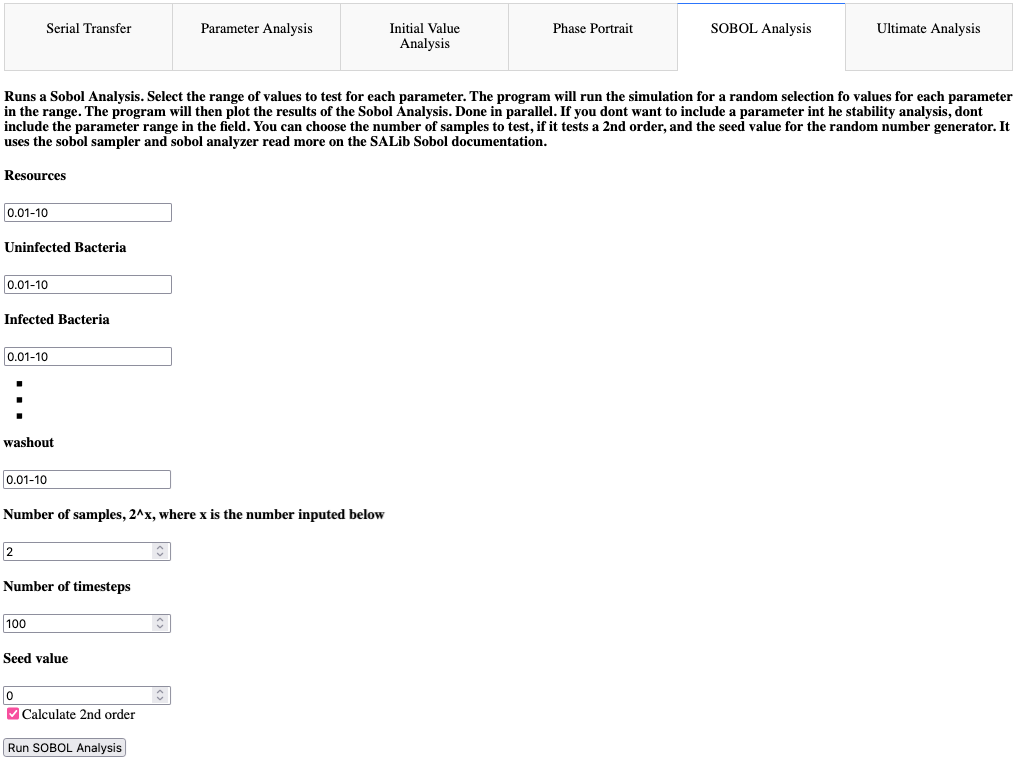
\includegraphics[width=\linewidth]{Screenshots/AdvancedVisualization/SOBOL_analysis_settings.png}
        \caption{
            The SOBOL settings tab. 
        }
        \label{fig:ss:av:SOBOL_analysis_settings}
    \end{subfigure}
    \hfill
    \begin{subfigure}{0.49\linewidth}
        \centering
        \captionsetup{width=1\linewidth}
        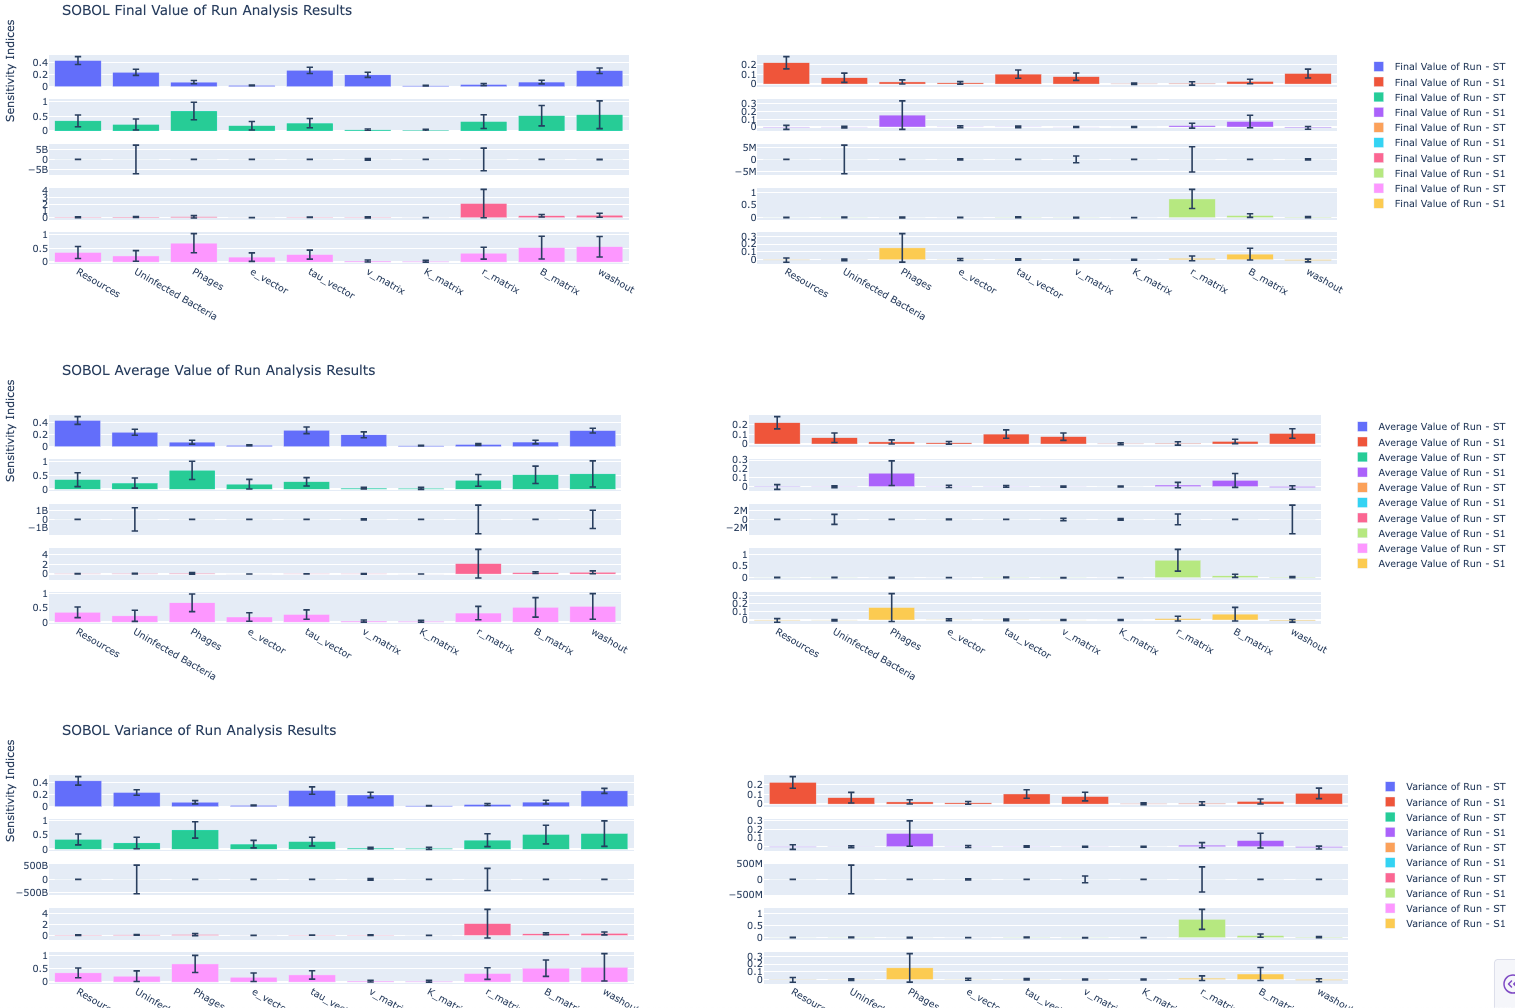
\includegraphics[width=\linewidth]{Screenshots/AdvancedVisualization/SOBOL_analysis_run.png}
        \caption{
            The output that can be expected from SOBOL. 
        }
        \label{fig:ss:av:SOBOL_analysis_run}
    \end{subfigure}
    \caption{SOBOL variance analysis}
\end{figure}

\paragraph{Ultimate Analysis}
\label{sec:ultimate_analysis}
The Ultimate Analysis section does not produce any visualizations or analysis, but instead allows for the user to define which initial conditions and parameter values they want to run a simulation on.
The solver will iterate over every single parameter input possibility and save the results in a \textit{.parquet} file.
Similarly settings in the other sections, the user can specify a start and end value, along with the number of values to generate evenly spaced within that range, including both the start and end values (\Cref{fig:ss:av:ultimate_analysis_settings}).
\newline
Using Dask and the saved \textit{.parquet} file, the user can query for specific runs, for example runs where a parameter value was greater than 0.05, and use the simulation data to create their own plots.
\begin{figure}
    \centering
    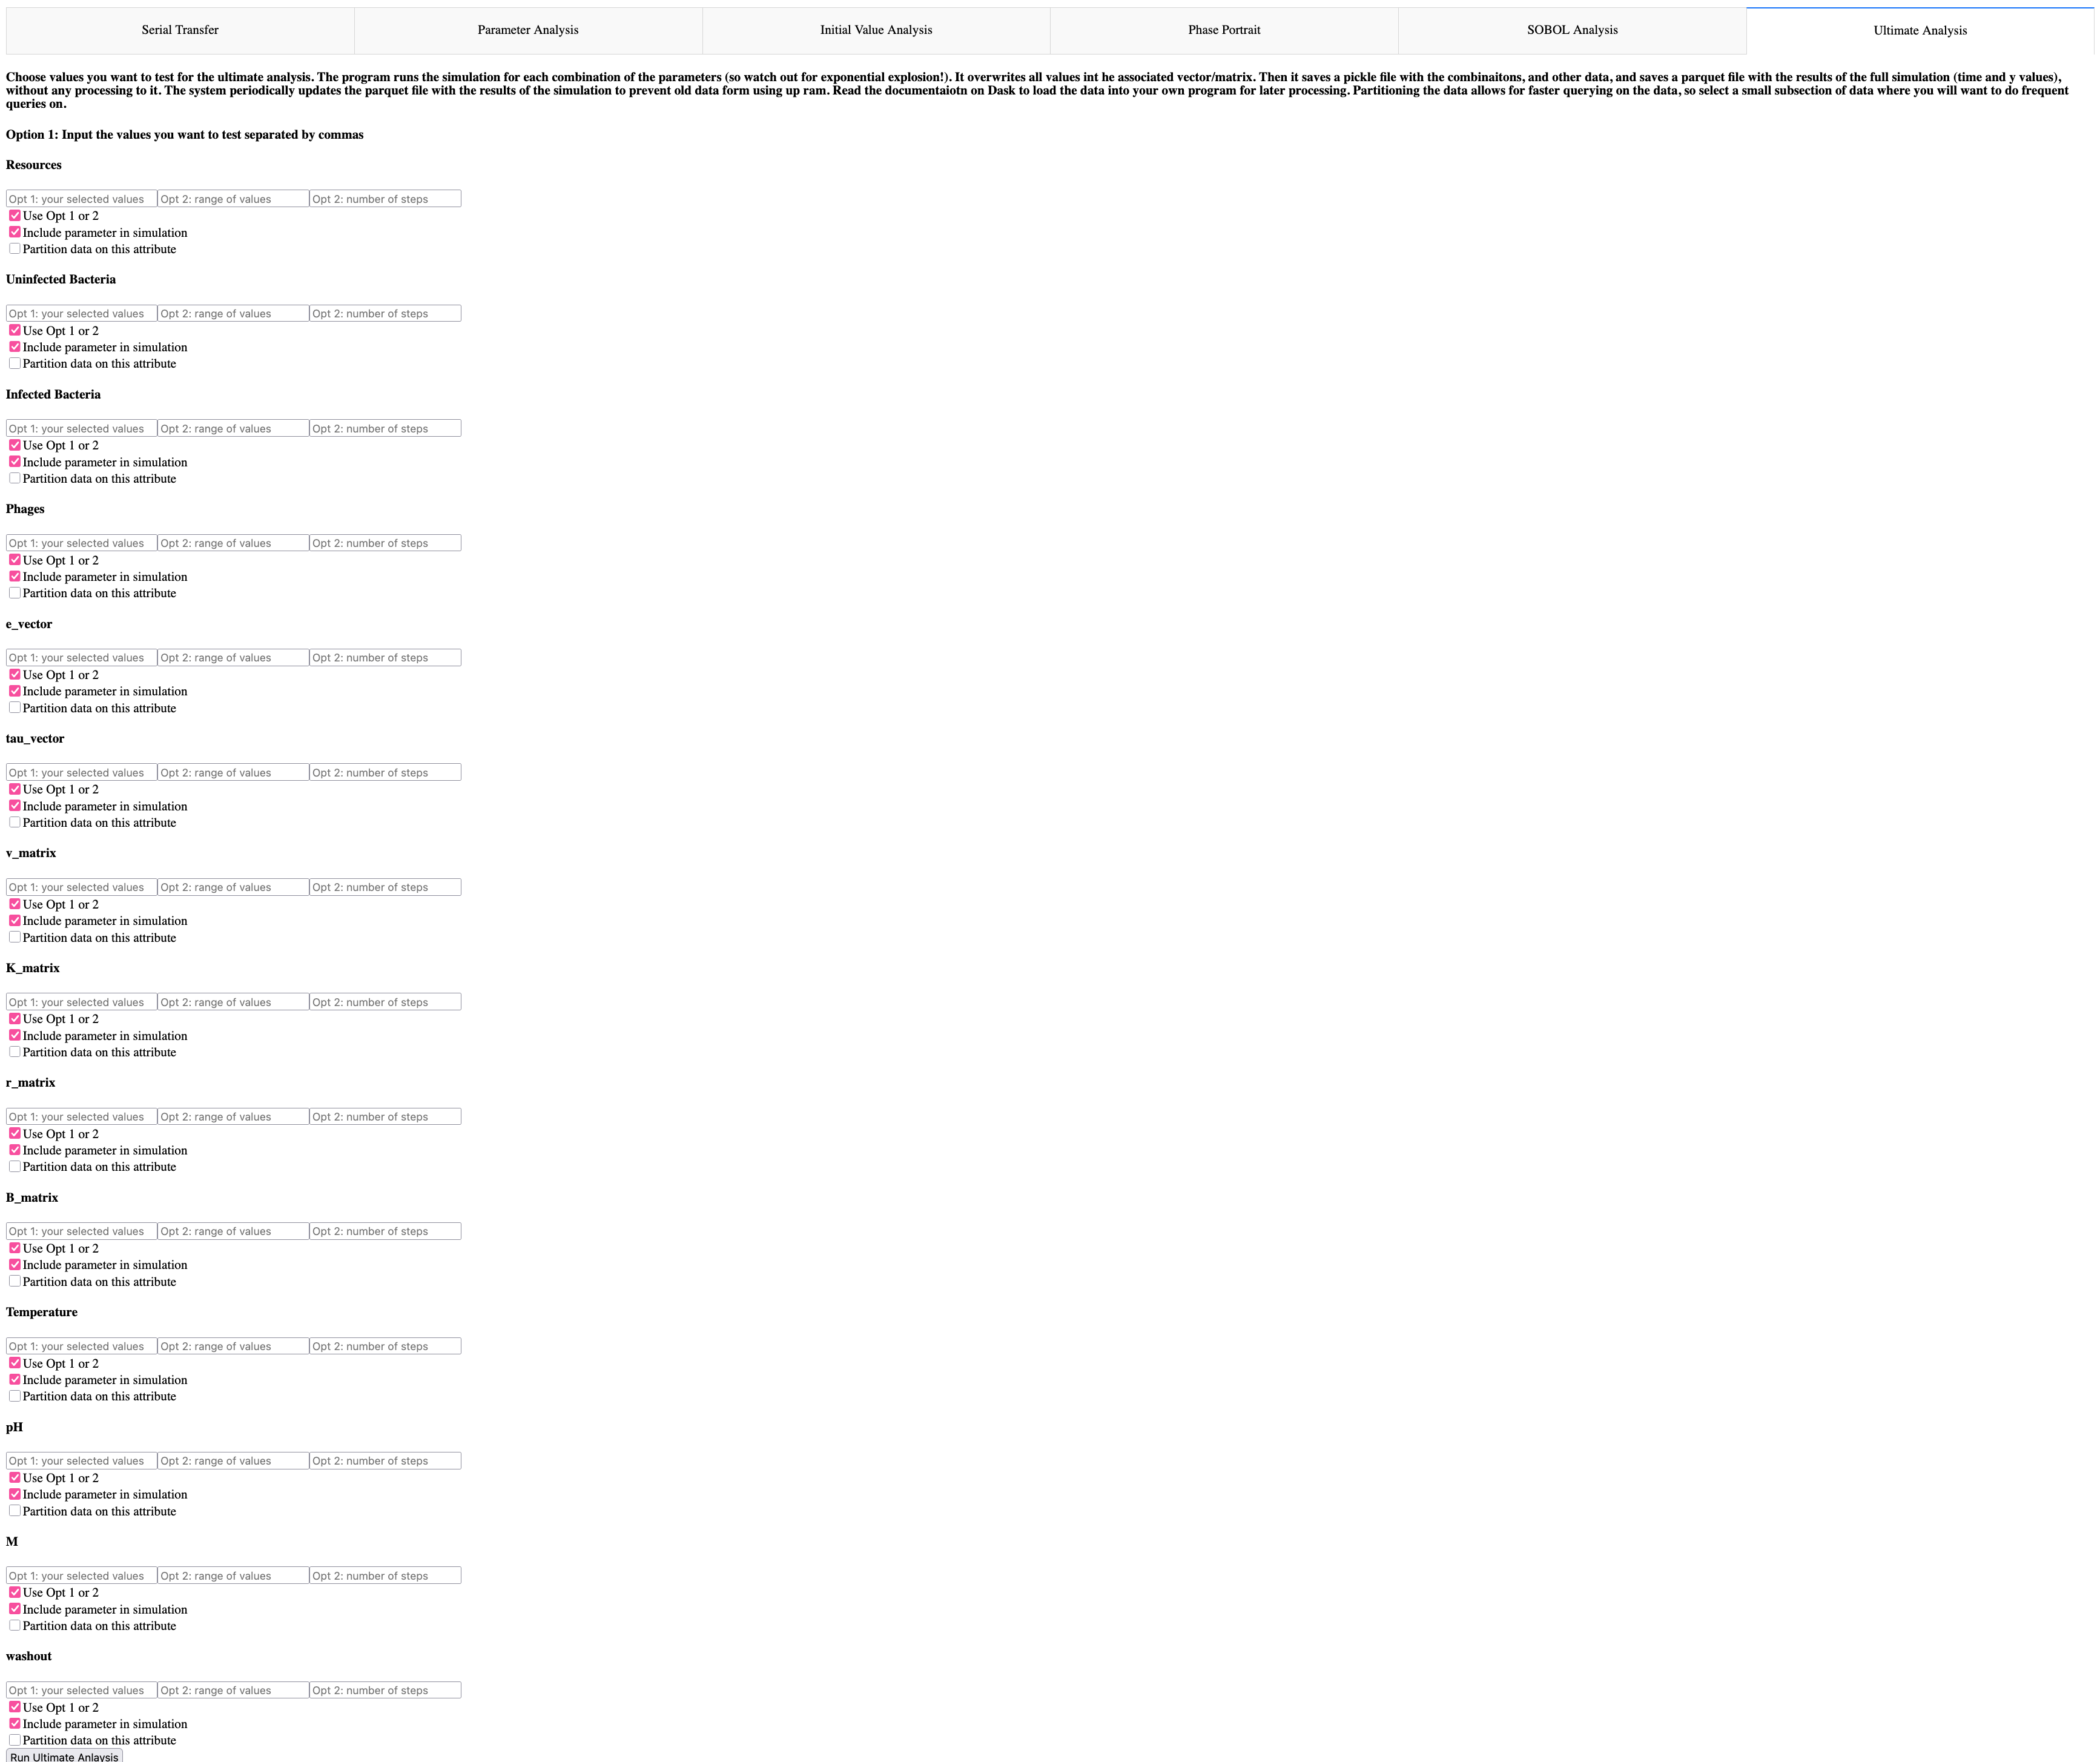
\includegraphics[width=1\linewidth]{Screenshots/AdvancedVisualization/ultimate_analysis_settings.png}
    \caption{
        The ultimate analysis setup tab. 
    }
    \label{fig:ss:av:ultimate_analysis_settings}
\end{figure}

\subsection{Custom Visualizations and Analyses} 
\label{sec:custom_visualizations_and_framework}
The final part, an optional step, allows the user to define a number of parameters they want to simulate and download the simulation results. 
The user can use this data to create their own custom visualizations without having to rerun the simulations, especially if there are many simulations. 
The data can be further processed and visualized as the user wishes. 

Depending on the provided model, different behavior might appear. 
As the dashboard can not create a graph for every situation, or be easily adapted to analyze every situation, \nameref{sec:ultimate_analysis} can be used to run and download the simulation data to the disk to later create your own custom visualizations. 
For example the agents in a model can exhibit cyclic behavior. 
A custom visualization that the could be created for this cyclic model would be to perform a Fourier transformation on the curve to obtain the predominant frequencies. 
A change in parameter values would change the frequencies of the curve, so it would be easy to quantify how a change in parameter value affects the frequency output. 
If dampening occurs, then a change in amplitude can also be measured, and compared to the change in frequency, allowing the user to identify if the frequency-dampening relationship is correlated or not. 

\section{Software Used and Packages}
The program was created exclusively in Python \cite{Python}, and makes extensive usages of various packages, ranging from the standard scientific packages such as NumPy \cite{NumPy} and SciPy to more niche packages such as pickle and SALib \cite{iwanagaSALib20Advancing2022, hermanSALibOpensourcePython2017}.

The graphical tool uses Tkinter acting as the front end, handling the user inputs, while NetworkX \cite{hagbergExploringNetworkStructure2008} stores the graph and contains the attribute data. 
The GUI tool also uses Matplotlib \cite{Matplotlib}to create the figure of the graph to display to the user in the GUI tool.

The simulation framework, the backend of the modelling, makes extensive usage of SciPy's \textit{solve\_ivp()} to create the ODE data. 
It also makes light usage of NetworkX to load the graph, as it initially takes a graph as an input, and light usage of NumPy to setup the parameters at startup. 

The visualization part makes heavily usage of Dash and Plotly. 
Dash acts as the server and is used for displaying the HTML aspect of the frontend and dealing with any input and output. 
Upon choosing parameter values and clicking on “submit“, Dash registers the activity and calls the function registered to the button, sending data such as parameter values and options like "log x-axis" form the frontend to the backend server. 
In the backend, the various inputs are handled, like changing the input string “0.05, 0.1, 0.15, 0.2” into an iterable list [0.05, 0.1, 0.15, 0.2] that the simulation framework can iterate over to vary the parameter value. 

If there are many simulations to run through, in the case of \nameref{sec:ultimate_analysis}, an intermediate call to a parallel computing library Joblib is called, where Joblib parallelizes the for-loop to compute the simulations in parallel. 

Ultimate analysis uses Pandas to write the data to a \textit{.parquet} file. 
Pandas parquet offers efficient data compression, efficient memory usage and when combined with Dask, efficient querying functionalities in a Dataframe format that many data scientists would be familiar with. 

SOBOL uses the SALib library to sample and analyze the parameter input. 
Both ultimate analysis and SOBOL save a \textit{.pickle} file containing a dictionary with the parameter values tested, setting values, and other important information regarding the simulation. 

\nameref{sec:initial_value_analysis} uses SciPy's \textit{curve\_fit()} function to curve fit the points in the middle plot (\Cref{fig:ss:av:initial_value_analysis_run}). 

Other packages that are used include collections, copy, warnings, itertools, os, datetime, json, gc, and time.  %Details of your approach (10-15 pages)
\lhead{\emph{Experiments and Results}}
\input{Chapters/ExperimentsandResults} %Evaluation/testing of your hypothesis (10-15 pages)
\lhead{\emph{Discussion}}
\chapter{Discussion}
\label{Discussion} %Evaluation/testing of your hypothesis (5-8 pages)
\lhead{\emph{Conclusions and Future Work}}
\input{Chapters/ConclusionsandFutureWork} % (5-6 pages)
\lhead{\emph{Ethics and Datamanagemnt}}
\lhead{\emph{}}
\chapter{Ethics and Data Management}
\label{edm}
\section{Ethical Considerations}
There are some ethical considerations needed. 
Phages can be used to treat bacterial infections and may need to be administered under the supervision of a doctor. 
Attempting to control phages in food or the environment by releasing a phage cocktail into waterways could cause issues further down the line if the released solution contains unwanted chemicals. 
An imbalance can be introduced into the ecosystem, further exacerbating the problem. 
An additional step in the food production process will increase food costs and make food production more difficult to control. 
The cost of creating, maintaining, and using phages at an industrial scale can become substantial and require a significant amount of energy. 
Dumping phages into the ecosystem could cause issues if the phage concoction includes resources that the bacteria can use, and this can become costly for taxpayers. 

\section{Data Management}
All data and results can be found on \href{https://github.com/BiggusVickus/Master-Thesis}{GitHub}. 
Some simulation data will have to be recreated as the \textit{.parquet} data files are too big for GitHub to store. 
Measures have been taken to label and document the code, datasets, and parameter configurations, for example, as shown in \Cref{AppendixE}. 
Any qualified researcher should be able to replicate, audit, use, and edit the computational experiments and code if needed. 
This systematic approach to version control and storage aligns with best practices, ensuring that results are both traceable and verifiable. 

\section{Adherence to Codes and Principles}
I acknowledge that the thesis adheres to the \href{https://student.uva.nl/en/topics/ethics-in-research}{ethical code} and \href{https://rdm.uva.nl/en}{research data management policies} of UvA and IvI.

The following table lists the data used in this thesis, with the source code. 
I confirm that the list is complete and that the listed data are sufficient to reproduce the results of the thesis. 

\begin{table}[ht!]
    \begin{tabular}{|l|l|l|}
    \hline
    \textbf{\begin{tabular}[c]{@{}l@{}}Short description \\ (max. 10 words)\end{tabular}} & \textbf{\begin{tabular}[c]{@{}l@{}}Availability \\ (e.g., URL, DOI)\end{tabular}} & \textbf{\begin{tabular}[c]{@{}l@{}}License \\ \end{tabular}} \\ \hline
        Dataset & \href{https://github.com/BiggusVickus/Master-Thesis/tree/main/SimulationResults}{Simulation Results} & MIT \\ \hline 
        Source Code & \href{https://github.com/BiggusVickus/Master-Thesis}{Source Code} & MIT \\ \hline
        Simulation Conditions & \Cref{AppendixE} and text under figures and in the text& \\ \hline
    \end{tabular}
\end{table} 

%----------------------------------------------------------------------------------------
%	THESIS CONTENT - APPENDICES
%----------------------------------------------------------------------------------------

%\addtocontents{toc}{\vspace{2em}} % Add a gap in the Contents, for aesthetics

%\appendix % Cue to tell LaTeX that the following 'chapters' are Appendices

% Include the appendices of the thesis as separate files from the Appendices folder
% Uncomment the lines as you write the Appendices

\lhead{\emph{Appendix A}}
\chapter{Appendix A: Equation Parameters}

\label{AppendixA}

Parameters used in equations. 

\begin{table}[htbp]
    \small % or \footnotesize to make it more compact
    \centering
    Golden Model
    \begin{tabularx}{\textwidth}{l l X}
        \toprule
        \textbf{Variable} & \textbf{Name} & \textbf{Description} \\
        \midrule
        $P_p$ & Phages agent & Phage population for phage $p$ \\
        $U_b$ & Uninfected Bacteria agent & Uninfected population for bacteria $b$ \\
        $I_{b_i}$ & Infected Bacteria agent & Infected population for bacteria $b$ at stage $1, \dots, i, \dots, M$  \\
        $B_b$ & Bacteria agent & Total bacteria population for bacteria $b$, assuming $B_b = U_b + \sum_{i=1}^M I_{b_i}$ \\
        $R_r$ & Resource agent & Resource $r$ concentration\\
        $e_{b, r}$ & Consumption rate& \\
        $\beta_{p, b}$ & Burst size & Lytic burst size for phage $p$ and bacteria $b$\\
        $r_{p, b}$ & Successful phage/cell encounter & Probability of a successful bacteria $b$ infection from phage $p$\\
        $\tau_{b}$ & Latent period & Time it takes bacteria $b$ to go through one infection stage\\
        $v_{b, n}$ & Maximal growth rate & Growth rate of bacteria $b$ from resource $r$ \\
        $K_{b, n}$ & Monod Constant & Monod constant for resource consumption rate dependent on resource $r$ concentration\\
        $\omega^i_r$ & wash-in rate & Rate of resources $r$ being added\\
        $\omega^o$ & wash-out rate & Rate of agents being removed, acts on all agents equally\\
        $M$ & Number of infection stages & Number of infection stages that a bacteria goes through, constant for all bacteria agents\\
        $t$ & time & time value \\
        \bottomrule
    \end{tabularx}\newline

    SOBOL
    \begin{tabularx}{\textwidth}{l l X}
        \toprule
        \textbf{Variable} & \textbf{Name} & \textbf{Description} \\
        \midrule
        $Y$ & Univariate parameter output & univariate model output, such as mean $\mu$ or variance $\sigma$ \\
        $X$ & Input vector & Vector of size $d$, input vector to $f$\\
        $X_i$ & Parameter input & Value of vector $X$ at position $i=1, \dots, d$ \\
        $d$ & Input size & Size of input vector $X$\\
        $X_{\sim i}$ & Parameter input & All values of $X$ that are not $X_i$ \\
        $f$ & Function $f$& Arbitrary black-box function describing model \\
        $N$ & Samples & Number of samples, power of 2, $2^x$ \\
        $D$ & Parameter input size & Number of parameters inputted into SOBOL, $d$ \\
        $S_{T_i}$ & Global sensitivity & Contribution of $X_i$ to output variance of $Y$ due to interactions with other variables  \\
        $S_i$ & First order sensitivity & Contribution of $X_i$ to output variance of $Y$ \\
        \bottomrule
    \end{tabularx} \newline

    Linear Regression
    \begin{tabularx}{\textwidth}{l l X}
        \toprule
        \textbf{Variable} & \textbf{Name} & \textbf{Description} \\
        \midrule
        $a$ & slope of linear regression line \\
        $c$ & Intercept of linear regression line\\
        $R^2$ & Coefficient of determination of linear regression fit, quality of regression \\
        \bottomrule
    \end{tabularx}
    \caption{Model parameters with variables, names, and descriptions. Subscripts on parameters indicate relationships; for example, $e_{b, r}$ is nonzero if there is an edge connecting bacteria $b$ to resource $r$ in the network, zero otherwise.}
    \label{tab:parameters}
\end{table}

\lhead{\emph{Appendix B}}
\chapter{Appendix B: Industrial and Real Life Applications of Phages} 
\label{AppendixB} 

Due to the nature of killing bacteria, there are numerous applications where a researcher or an organization might be interested in controlling bacterial populations.

A Food Safety Specialist might be interested in introducing a solution containing a high concentration of phages during food production to prevent the spread and growth of \textit{Salmonella} or \textit{E. coli} in the pet food. 
Alternatively, the Food Safety Specialist might want to promote beneficial bacteria like \textit{Streptococcus thermophilus}, used in the production of Emmental cheese, which heat would kill during the pasteurization process. 

A doctor might be interested in providing swallowable pills, more commonly known as phage cocktails, to a patient with a bacterial infection.
There is evidence that phage-resistant bacteria are more susceptible to antibiotics; therefore, the doctor might prescribe both medicines to treat the infection effectively. 

An Environmental Protection Officer might be interested in seeing how they can use phages to stop the spread of \textit{Cyanobacteria} blooms in waterways, more commonly known as blue-green algae, a photosynthetic microscopic organism that is technically classified as a type of bacteria.
This would keep waterways safe for boating and swimming activity, aquatic life, and water consumption in farms, factories, and homes. 

When there are a few known bacterial strains, a targeted cocktail of phages can be used to control bacterial population growth in any setting, whether it be food, healthcare, or the environment.
Phages offer properties of microbial control that other methods do not, making them an ideal candidate for some applications. 

\section{Controlling Foodborne Bacteria}
\label{sec:AppendixB:controlling_foodborne_bacteria}
Foodborne diseases are one of the primary ways for bacteria to spread to humans and animals.
Some bacteria use the food as a vector to infect hosts, while others deposit toxins on the food, which is then ingested.
If consumed in large enough quantities or further produced in the host, the toxins can be fatal to the host.

Methods exist to control bacterial growth, for example, by storing food at temperatures below 5\textdegree C or above 60\textdegree C.
Bacteria need moisture to grow, so starches like rice will have minimal bacterial growth.
Bacteria prefer to live in slightly acidic to neutral pH environments; therefore, having an extremely acidic environment, such as vinegar, will prevent bacterial growth.
The use of chemical antibacterial agents, such as bleach, is undesirable due to the potential for leaving residues on food, which can be fatal if ingested.
Physical entities like heat or radiation can kill bacteria, but at the cost of altering the food quality \cite{fieseler_food_2021}. 

For example, \textit{Streptococcus thermophilus} is one of three different bacteria strains used to create Emmental cheese.
However, Emmental cheese does not use pasteurized milk, which increases the risk of \textit{E. coli}.
Emmental cheese producers can add phages that target \textit{E. coli} to the milk during the production stage while not affecting the bacteria used to produce the cheese. 

\subsection{Current Applications}
Phage cocktails like SalmoFresh\textsuperscript{TM} have been proven to safely reduce \textit{Salmonella} contamination in pet food and raw pet food ingredients \cite{sofferBacteriophagesSafelyReduce2016}, as well as in romaine lettuce and bean sprouts \cite{zhangSalmoFreshEffectivenessControlling2019}.
Pet food contains meat and vegetables, where vegetables grown in or on the ground are at risk of \textit{Salmonella} due to contact with soil, manure, compost, and other agricultural runoff from neighboring farms \cite{kowalskaFreshVegetablesFruit2023}.
\Cref{fig:SalmoFresh_in_pet_food} and \Cref{fig:SalmoFresh_effectiveness_lettuce_sprouts} show how the application of phages has reduced the count of \textit{Salmonella} in ingredients used in pet food as well as romaine lettuce and bean sprouts. 
In \Cref{fig:SalmoFresh_in_pet_food}, each food group noticed at least a 68\% reduction in CFU/g compared to the control when the $9\times 10^6$ phage treatment was applied. 
There was at least an 80\% reduction in CFU/g across all food groups when treated with a concentration of $9\times 10^6$ or stronger. 
In \Cref{fig:SalmoFresh_effectiveness_lettuce_sprouts}, the lettuce and bean sprouts noticed a reduction of at least 0.6 log CFU/mL in \textit{Salmonella} count across all temperature ranges. 
The most significant reduction in bacterial count in lettuce was observed at 1 hour at 2\textdegree C with an absolute reduction of 62.0\% between the control and treatment. 
The most significant reduction in bacteria of 90.0\% was observed at 72 hours at 2\textdegree C. 
For the bean sprouts, the lowest reduction in phages was found at 1 hour at 2\textdegree C with a reduction of 78.1\%, and the most significant reduction was 90.0\% at 25\textdegree C after 48 hours. 
Although these values are still above the food-safe threshold, the ability to reduce the \textit{Salmonella} population by at least 62\% and up to 90\% at various temperatures and incubation periods is impressive. It can prolong shelf life, especially for foods that have short shelf lives before spoiling due to bacterial growth. 
As such, phages can be shown to control the spread of \textit{Salmonella} in food sources and extend the potential shelf life of certain foods. 

\begin{figure}[ht!]
    \centering
    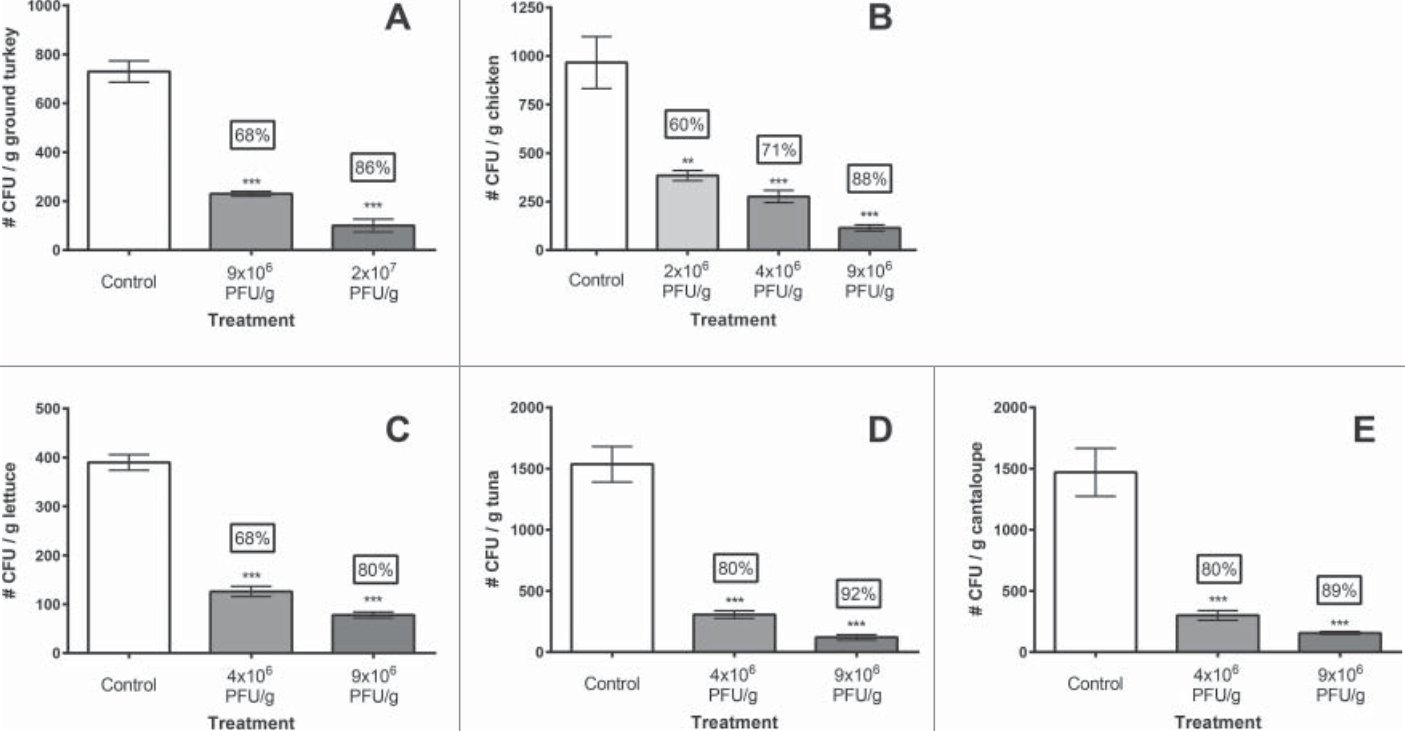
\includegraphics[width=0.5\linewidth]{Plots/Sourced/SalmoFresh_in_pet_food.png}
    \caption{SalmoLyse\textsuperscript{\textregistered} reduces Salmonella contamination on various food surfaces: Mean and standard error bars shown.
 Statistical analyses were carried out for each food group independently.
 Asterisks denote significant reduction from corresponding controls based on one-way ANOVA with Tukey’s post-hoc tests for multiple corrections: ** denotes $p < 0.01$, while *** denotes $p < 0.001$ compared to the corresponding controls.
 There was a significant reduction in Salmonella on all food surfaces with the addition of SalmoLyse\textsuperscript{\textregistered} compared to the controls; the mean percent reductions from the control are noted in the boxes above treatment bars.
 CFU/g D colony forming units per gram.
 Each letter denotes a food group that was tested with SalmoLyse\textsuperscript{\textregistered} and compared to a control: A= chicken; B= lettuce; C= tuna; D= cantaloupe; E= ground turkey. Plot sourced from \citet{sofferBacteriophagesSafelyReduce2016}. 
 }
    \label{fig:SalmoFresh_in_pet_food}
\end{figure}

\begin{figure}[ht!]
    \centering
    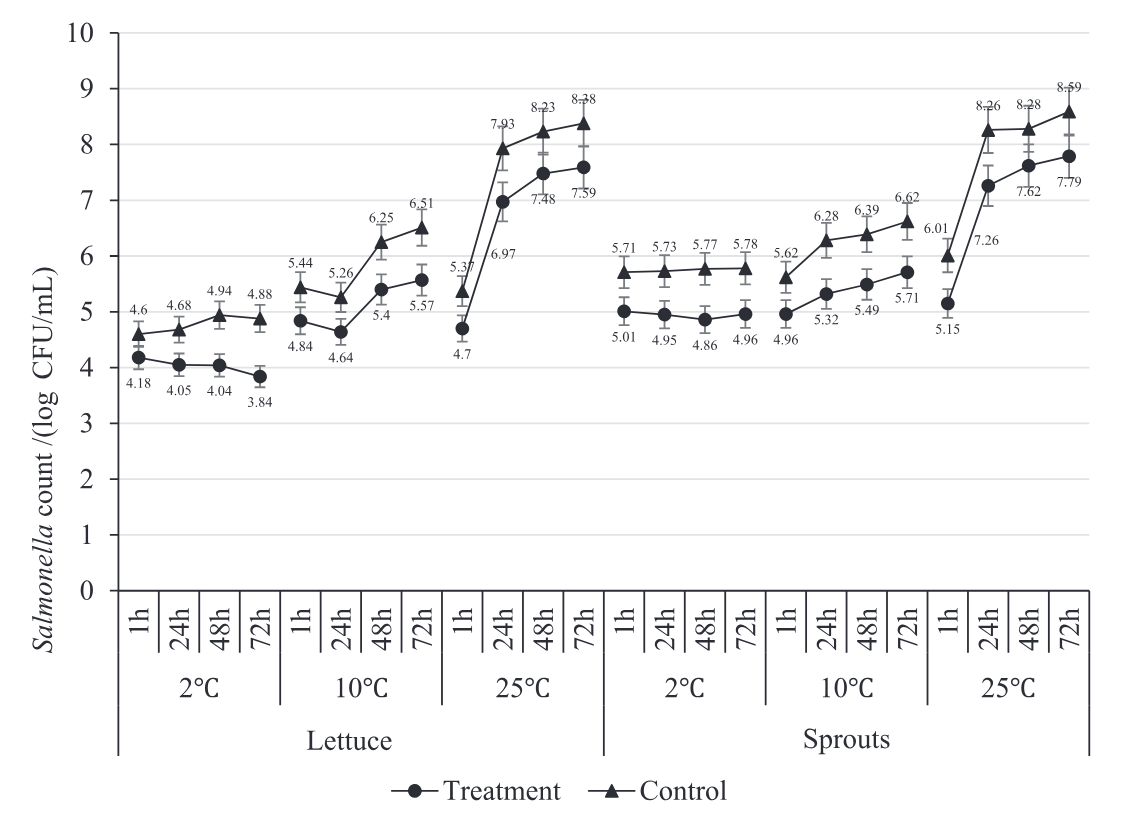
\includegraphics[width=0.5\linewidth]{Plots/Sourced/SalmoFresh_effectiveness_lettuce_sprouts.png}
    \caption{\textit{Salmonella} count in a mixture of 5 \textit{Salmonella} strains spot-inoculated (CFU/g) onto a) lettuce and b) sprouts after spraying with a mixture of bacteriophage (SalmoFresh\textsuperscript{TM}) relative to positive controls at 2, 10 and 25C and stored for 1, 24, 48 and 72 h. Plot sourced from \citet{zhangSalmoFreshEffectivenessControlling2019}}
    \label{fig:SalmoFresh_effectiveness_lettuce_sprouts}
\end{figure}


\section{Phage Therapy and Antibiotics}
\label{sec:AppendixB:phage_therapy_and_antibiotics}
Antibiotics are a common treatment for bacterial infections.
However, antibiotics are not selective in the bacteria they kill, killing both harmful and beneficial bacteria.
This can lead to the development of antibiotic-resistant bacteria, which makes it harder to combat those bacteria in the future.
It has also been demonstrated that antibiotics can harm the gut microbiome and brain development in mice.
Phages are an alternative to antibiotics, as they are selective in the bacteria they kill and do not interact with cells or other important biological functions.
The rise in antibiotic-resistant bacteria can be attributed to the overuse and overprescription of antibiotics, as well as incorrect usage (for example, prematurely stopping) \cite{odonkorBacteriaResistanceAntibiotics2011}.
These actions exert evolutionary pressure on bacteria to mutate and develop resistance to antibiotics. 
Phage therapy can contain any number of different phages that target specific bacterial infections, such as \textit{Streptococcus pneumoniae}, with minimal risk of side effects.

\subsection{Current Applications: Bacterial Infection Control}
One active area of research is the use of phages to control bacterial infections.
Due to the specificity of phages, they can be used to target specific bacteria strains without affecting other beneficial bacteria.
When sick with a bacterial infection, patients swallow antibiotic pills to help the body fight the infection.
Antibiotics work by either interrupting intercellular processes like the synthesis of RNA \cite{flossRifamycinModeActionResistance2005}, by disrupting the structural integrity of the cell wall \cite{tomaszMechanismIrreversibleAntimicrobial1979}, or by inhibiting protein synthesis \cite{vakulenkoVersatilityAminoglycosidesProspects2003}.

However, antibiotics are not strain-specific and indiscriminately kill other bacteria as well.
Common side effects of antibiotics, although usually not serious, include diarrhea, nausea, and headaches.
It has also been shown that the effects of early-stage penicillin exposure in mice have been found to have a long-lasting effect on the gut microbiome, frontal cortex gene expression, and amygdala gene expression \cite{volkovaEffectsEarlylifePenicillin2021}.
Penicillin increases cytokine expression (small proteins involved in cell signaling) in the frontal cortex of the brain, modifies the integrity of the blood-brain barrier, and alters behavior.
The mice exhibited an increase in aggression and anxiety-like behavior \cite{leclercqLowdosePenicillinEarly2017}.
Phages can be used as an alternative to antibiotics, offering benefits without side effects and without affecting the gut microbiome. 

With an increase in antibiotic use, there has been a corresponding rise in antibiotic-resistant bacteria.
The World Health Organization has stated that antibiotic resistance poses a significant threat to modern medicine and the sustainability of an effective, global public health response to the enduring challenge of infectious diseases.
Common infections that previously would have been easy to treat are more complicated to treat and can increase the risk of disease spread, severe illness, and death \cite{GlobalActionPlan}. 

One area of research is exploring how bacteria can exchange traits such as phage resistance and antibiotic resistance.
Some bacteria are multi-drug resistant and no longer respond to the medicine.

\citet{laurePhageResistancemediatedTradeoffs2022} showed evidence that \textit{Salmonella Typhimurium} is more susceptible to ampicillin in the presence of phages, and phage-resistance can lead to reduced virulence and decreased antibiotic resistance. 

\citet{zhaoPhagedrivenCoevolutionReveals2024} showed that there exists an antagonist coevolution between the bacteria and phages, where the dynamics changed from an arms race dynamic (ARD) to a fluctuating selection dynamics (FSD).
Due to phage selection and bacterial competition pressure, when bacteria gained phage resistance, they often lost antibiotic resistance.
Genome analysis revealed mutations in the \ textit {btuB} gene of \textit{Salmonella anatum}, with a higher mutation frequency during the ARD stage.
A knockout experiment confirmed that the btuB gene is a receptor for the \textit{JNwz02} phage, resulting in reduced bacterial competitiveness.
Further analysis detected multiple single nucleotide polymorphism (SNP) mutations in the phage-resistant strains.
The SNPs potentially affected the membrane components, partially weakening the cell defense against antibiotics.
These findings help advance our understanding of phage-host-antibiotics interactions and the impact of adaptations to antibiotic resistance.
The research demonstrates how phages can be utilized to reintroduce antibiotic susceptibility to previously insusceptible bacteria, thereby preventing costly and lengthy research on new antibiotics \cite{zhaoPhagedrivenCoevolutionReveals2024}. 

Phage research is facing challenges due to bacterial strains evolving resistance to phages.
Understanding the interplay between antibiotics and phages is essential for shaping future research \cite{zhaoPhagedrivenCoevolutionReveals2024}.


\section{Environmental Protection}
\label{sec:AppendixB:environmental_protection}
Algae blooms, also called red tides, is the rapid spread of bacterial or algae organisms.
Blooms are a growing environmental concern impacting water quality, aquatic ecosystems, and human health.
These rapid increases in algae populations, often fueled by excess nutrients such as nitrogen and phosphorus, can occur in freshwater, coastal, and marine environments. 

Cyanobacteria blooms have significant impacts on both the aquatic environment and human health.
Cyanobacteria release nitrogen and phosphorous, which the bacteria use to grow with oxygen, outpacing other aquatic growth and killing aquatic marine life.
Bacterial toxins can make their way into the food and water consumed by humans, causing muscle fatigue, respiratory issues, liver damage, and gastrointestinal issues \cite{zhangImpactCyanobacteriaBlooms2022}.
\Cref{fig:cyanobacteria_bloom_cycle} shows the process of how cyanobacteria degrade and are absorbed into the environment, eventually making their way into the human body via various contact points.
 
\begin{figure}
    \centering
    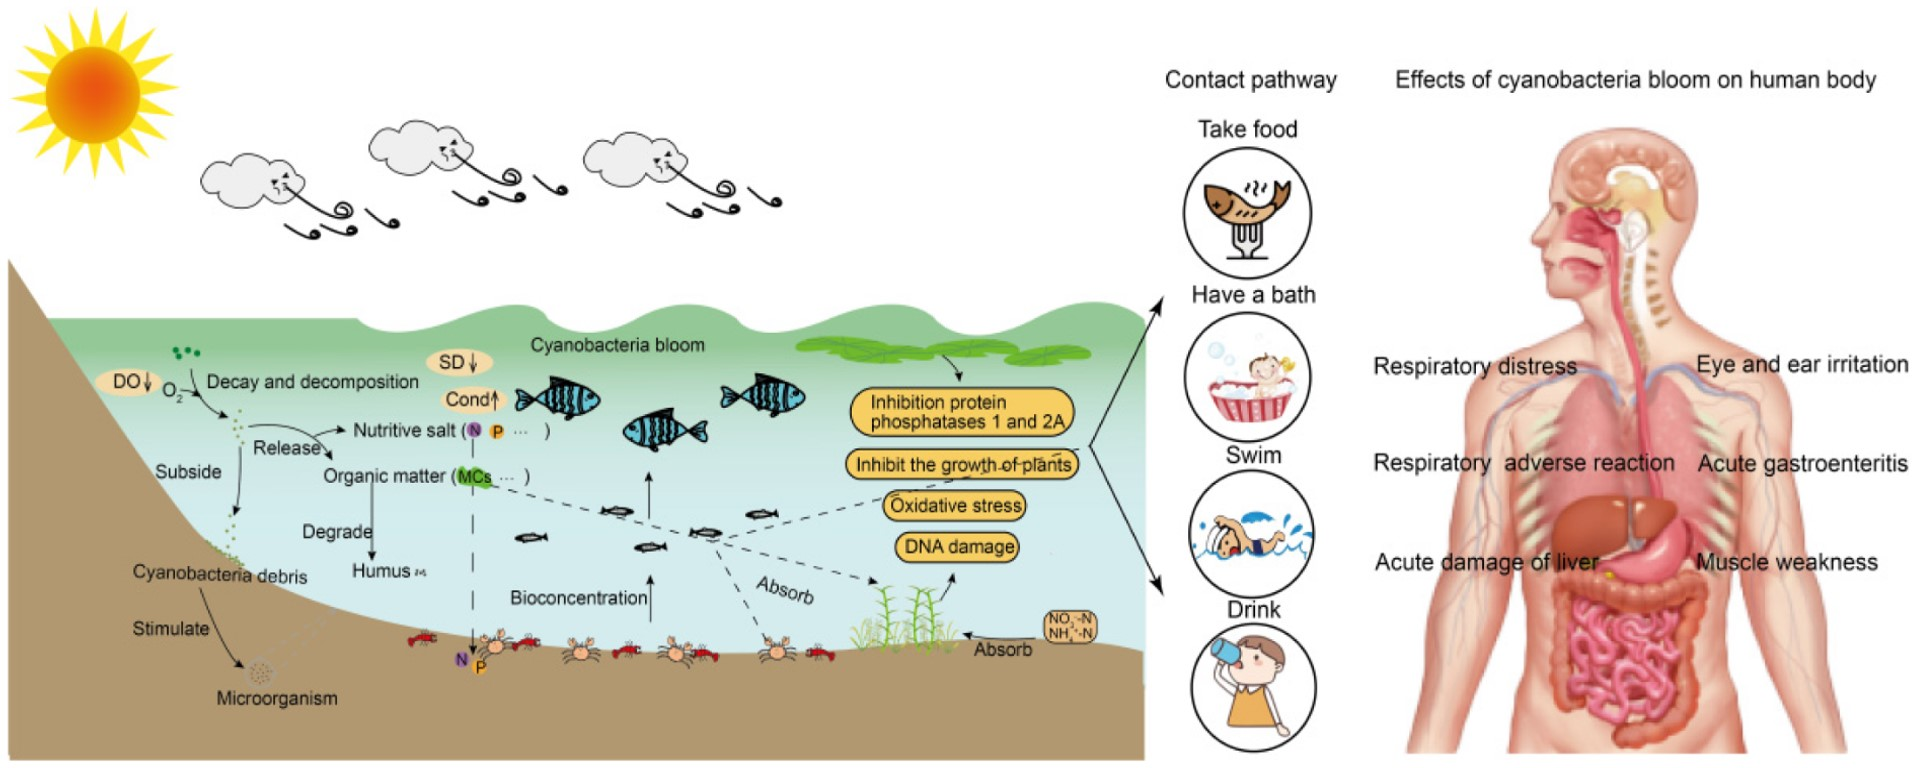
\includegraphics[width=0.75\linewidth]{Figures/cyanobacteria_bloom_cycle.png} 
    \caption{Cyanobacteria degradation cycle, main hazards of cyanobacteria bloom to water bodies, aquatic organisms, and the human body. (DO: dissolved oxygen; SD: water transparency; Cond: conductivity; N: nitrogen; P: phosphorus; MCs: microcystins). \cite{zhangImpactCyanobacteriaBlooms2022}}
    \label{fig:cyanobacteria_bloom_cycle}
\end{figure}

\subsection{Current Applications}
 There is interest in using phages to control cyanobacteria blooms.
Phages can offer better and safer alternatives to chemical options when attempting to control bacterial blooms.
Chemical options are indiscriminate, killing cyanobacteria while also killing other beneficial bacteria and aquatic life, and can eventually seep into groundwater.
Although not used to control bacteria blooms, some chemicals like PFAS, also called “Forever Chemicals”, can last a long time in the environment and do not degrade and keep on negatively affecting the environment.
Due to the specificity of phages, only cyanobacteria will be targeted, and this will not affect the surrounding environment. 

Tucker and Pollard found that an isolated phage cocktail collected from Lake Baroon in Australia could decrease the abundance of \textit{M. aeruginosa} by 95\% within 6 days in a lab setting, before recovering within 3 weeks \cite{tuckerIdentificationCyanophageMaLBP2005}. 

There is evidence that phage-resistant bacteria can influence the population dynamics of other bacteria.
It has been shown that the plankton level has been experimentally affected by the frequency of the phage-resistant \textit{Nodularia} marine bacteria.
Populations with high phage resistance ($>50\%$) dominate the plankton communities despite a high phage count and eventually outcompete other bacteria due to their slower decline in population size.
Contrastingly, populations of bacteria with low phage resistance (between 0\% and 5\%) were lysed to extinction, releasing resources such as nitrogen.
This allows for other bacterial strains to absorb the resources and dominate the bacterial community.
Phages and the lysis of bacterial strains can have a dramatic effect on the community dynamics and composition of other entities, such as phages, bacteria, and resources \cite{colomaFrequencyVirusresistantHosts2019}.
Phages have the potential to be used as a specific strategy for controlling cyanobacterial blooms with minimal environmental impact, offering control of bacterial blooms with limited environmental impact.
Usage should be safe, novel, efficient, and sensitive.  

However, there are issues with using phages to control bacterial blooms.
Bacterial blooms can cover vast areas or occur in areas that are difficult to reach, such as marshlands; applying phages to combat the bloom may be infeasible.
If the method of choice were to spray a solution of water containing phages, the solution would need to be shipped to the site and loaded onto special boats to spray the solution into the water, or the trucks would need to drive along the shore and spray the solution into the water.
This solution may not address the root cause, for example, the constant discharge of wastewater into a river. 

The phage density in the solution must be relatively high to combat the bloom quickly.
These problems pose significant logistical challenges in creating the phages in a lab or factory, transporting them, and administering the phages to the waterways.
Phages can only diffuse through the water and cannot actively swim, so they are dependent on the rate of diffusion and water currents.
This will be difficult in marshlands, where the bacteria can “hide” in the grass and crevices created by aquatic life.
If the bloom occurs in a high-current area, such as a river or a bay, the water can wash the phages away.

Scientists have not yet fully understood the phage infection mechanism, and research into the artificial engineering of phages is limited, making it challenging to conduct studies in this area \cite{grassoReviewCyanophageHost2022, mckindlesDissolvedMicrocystinRelease2020}.
 
Algae can produce toxins that threaten wildlife, contaminate drinking water, and disrupt local economies dependent on fishing and tourism.
In the state of Florida, between the years 1995 and 2000, the restaurant and hotel industry lost an estimated $\$6.5$ million to algae blooms.
This accounts for approximately 25\% of the average total monthly sales revenue in the region from June through October, the months most commonly affected by red tide\cite{PDFEconomicImpacts}.
During a red bloom event, hospital diagnoses in the county of Sarasota for pneumonia, gastrointestinal, and respiratory illness increased by 19\%, 40\% and 54\% respectively \cite{chengCharacterizationMarineAerosol2005, kirkpatrickGastrointestinalEmergencyRoom2010}, with a respiratory illness visit costing between $\$0.5$ and $\$4$ million \cite{hoaglandCostsRespiratoryIllnesses2009}. 
\lhead{\emph{Appendix C}}
\chapter{Appendix C: Flowchart of User and System Interactions}
\label{AppendixC}

\Cref{fig:interaction_diagram} shows how the user can interact with the system, the input and outputs for subsystems, and the systems working with one another. 
    To read the flow chart, start from the top to the bottom. 
    First the user creates a network using the GUI Network Creation Tool. 
    After the graph is finished, the user provides an implementation of the network as an ODE model, using Python. 
    Once finished, the user provides the network file and ODE model to the ODE solver. 
    The solver uses information from the network file to determine the number of entities to create, parameter details (including names, values, and dimensions), and setting values.
    Then the user interacts with the Visualization Dashboard Tool, for example by clicking on buttons to run simulations, changing parameter values, (un)selecting checkboxes, and zooming in and out of plots, and hovering over plots to show data. 
    Once a user has selected the parameter values, the parameter values are sent to the solver. 
    The solver calculates the time and population values using the provided graph and ODE model and sends the data back to the Visualization Dashboard Tool, which then outputs the visualizations. 
    If the user has run an ultimate analysis, then the user can query the saved data to make their own custom visualizations.
\begin{figure}
    \centering
    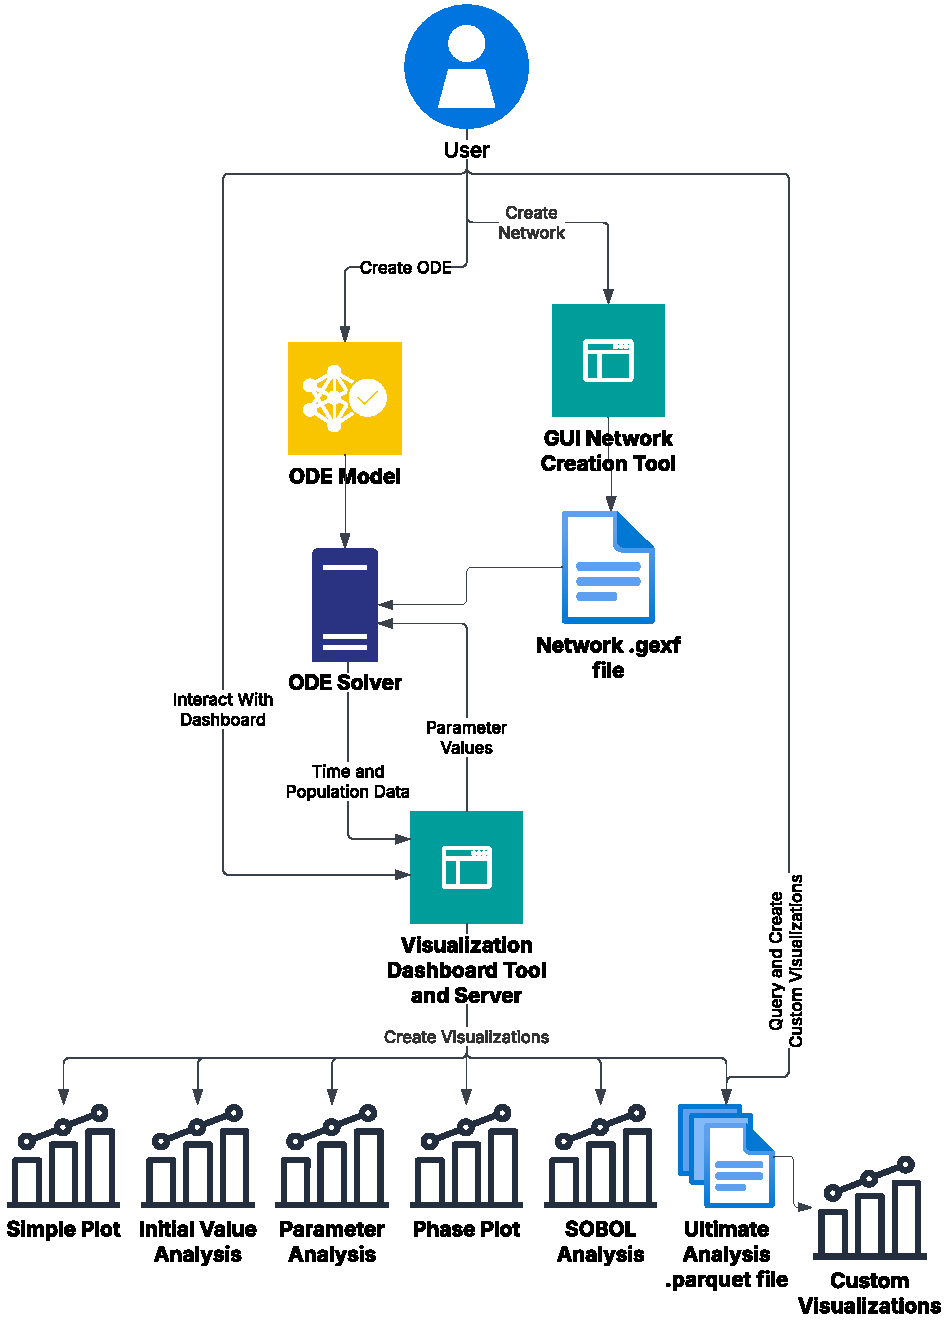
\includegraphics[width=0.8\linewidth]{Images/interaction_diagram.pdf}
    \captionsetup{width=1\linewidth}
    \caption{
        The flowchart of user and system interactions. Read from top to bottom. 
    }
    \label{fig:interaction_diagram}
\end{figure} 

\addtocontents{toc}{\vspace{2em}} % Add a gap in the Contents, for aesthetics

\backmatter


% \begin{figure}[!ht]
%     \centering
%     \begin{subfigure}{\linewidth}
%         \centering
%         \includegraphics[width=1\linewidth]{figure1.png}
%         \caption{caption text}
%      \label{fig:label1}
%      \end{subfigure} 
    
%     \begin{subfigure}{\linewidth}
%         \centering
%         \includegraphics[width=1\linewidth]{figure2.png}
%         \caption{caption text}
%         \label{fig:label2}
%     \end{subfigure}%
%  \end{figure}

% \begin{figure}[ht]
%     \centering
%     \subfloat[text here describing fig 1]{\includegraphics[width=0.4\textwidth]{figure1.png}}
%     \subfloat[text here describing fig 2]{\includegraphics[width=0.4\textwidth]{figure2.png}}
%     \hfill
%     \subfloat[text here describing fig 3]{\includegraphics[width=0.4\textwidth]{figure3.png}}
%     \subfloat[text here describing fig 4]{\includegraphics[width=0.4\textwidth]{figure4.png}}
%     \caption{Caption text}
%     \label{fig:streamlines}
% \end{figure}


%----------------------------------------------------------------------------------------
%	BIBLIOGRAPHY
%----------------------------------------------------------------------------------------

\label{References}

\lhead{\emph{References}} % Change the page header to say "Bibliography"

\bibliographystyle{unsrtnat} % Use the "unsrtnat" BibTeX style for formatting the Bibliography

\bibliography{References,References2} % The references (bibliography) information are stored in the file named "Bibliography.bib"
\end{document} 